\documentclass[10pt,a4paper,twoside,openright]{../llncs}

               %%%%%%%%%%%%%%%%%%%%%%%%%%%%%%%%%%%%%%
               %    Scelta dei package da usare     %
               %%%%%%%%%%%%%%%%%%%%%%%%%%%%%%%%%%%%%%

\usepackage[utf8,latin1]{inputenc}
%%\usepackage{amsmath,amsfonts,amssymb,amsthm}
\usepackage[english]{babel}
\usepackage[T1]{fontenc}
\usepackage{url}
\usepackage{xspace}
\usepackage{fancyhdr}
\usepackage{graphicx}
\usepackage{color}
%% \usepackage{lastpage} 
\usepackage{listings}
\usepackage{amssymb}    %%% by AN
\usepackage{fancyvrb}   %%% by AN
\usepackage{floatflt}   %%% by AN
\usepackage{hyperref}


%%%%%%%%%%%%%%%%%%%%%%%%%%%%%%%%%%%%%%%%%
% Java syntax in listings eclipse like	%
%%%%%%%%%%%%%%%%%%%%%%%%%%%%%%%%%%%%%%%%%
\definecolor{javared}{rgb}{0.6,0,0} % for strings
\definecolor{javagreen}{rgb}{0.25,0.5,0.35} % comments
\definecolor{javapurple}{rgb}{0.5,0,0.35} % keywords
\definecolor{javadocblue}{rgb}{0.25,0.35,0.75} % javadoc
\definecolor{eclipseKeyword}{RGB}{0,0,204}
\definecolor{eclipseComment}{RGB}{149, 0, 85}
\definecolor{eclipseString}{RGB}{153, 0, 153}
\definecolor{lightgray}{rgb}{0.98,0.98,0.98}
 
\lstset{language=java,
  basicstyle={\scriptsize\ttfamily},
  numbers=left,
  numberstyle=\tiny\color{black},
  %%backgroundcolor=\color{lightgray},
  showstringspaces=false,
  columns=flexible,
  keywordstyle={\color{eclipseKeyword}\textbf},
  %%keywordstyle=\color{javadocblue}\bfseries,
  %% commentstyle={\color{eclipseComment}\textit},
  commentstyle={\color{eclipseComment}},
  stringstyle={\color{eclipseString}},
  frame=single,
  breaklines=true,
  breakatwhitespace=true,
  tabsize=4,
  showspaces=false,
  showstringspaces=false,
  %% morekeywords={public, void, for, class, AsynchActionResult, },
  %% ndkeywords={Task,Behavior,Event},
  %% ndkeywordstyle={\color{darkgray}\bfseries},
  %% escapeinside={(*@}{@*)},
  captionpos=b
} 

\lstdefinelanguage{qa}{
 %%morecomment=[1]{//},
 morecomment=[s]{/*}{*/},
 morekeywords={RobotSystem,System,Context,Robot,QActor,Plan,context,resumeLastPlan,sound,time,
 forward, demand,receiveMsg,onMsg,EventHandler, Request, printCurremtMessage, printCurrentEvent, -memo,
 normal,file,regeneratesrc,host,port,println, switchToPlan , answerEv , onFailSwitchTo , repeatPlan ,
 memoCurrentEvent , memoCurrentMessage , robotForward, robotBackward, robotLeft, robotRight, robotStop , 
 java\_object , class , solve , Event , Dispatch , returns ,   
 }
} 
\lstdefinelanguage{pl}{
 %%morecomment=[1]{//},
 morecomment=[s]{\%}{\ },
 morecomment=[s]{//}{\ },
 morecomment=[s]{/*}{*/},
}  
\lstdefinelanguage{ddr}{
 %%morecomment=[1]{//},
 morecomment=[s]{/*}{*/},
 morekeywords={RobotSystem,System,Context,Robot,QActor,Plan,context,resumeLastPlan,sound,time,
 forward, demand,receiveMsg,onMsg,EventHandler,Request,printCurremtMessage,printCurrentEvent,
 normal,file,regeneratesrc,host,port,println, switchToPlan , answerEv , onFailSwitchTo , repeatPlan ,
 memoCurrentEvent , memoCurrentMessage , robotForward, robotBackward, robotLeft, robotRight, robotStop , 
 java\_object , class , solve , Event , Dispatch , returns ,   
 }
} 
 
\lstnewenvironment{javacode}{\lstset{language=Java}}{}
\lstnewenvironment{qacode}{\lstset{language=qa}}{}
 
%%%%%%%%%%%%%%%%%%%%%%%%%%%%%%%

\pagestyle{fancy}
\fancyhf{}
 
\rfoot{Page \thepage}

\makeatletter

\usepackage{../manifest}
%% \usepackage{../MyStyle}

\makeatother

               %%%%%%%%%%%%%%%%%%%%%%%%%%%%%%%%%%%%%%%%
               % Scelta delle dimensioni della pagina %
               %%%%%%%%%%%%%%%%%%%%%%%%%%%%%%%%%%%%%%%%

\setlength{\textwidth}{15,5cm}
\setlength{\textheight}{20cm} 
\setlength{\oddsidemargin}{0.1cm}
\setlength{\evensidemargin}{0.1cm}
\setlength{\footskip}{1cm}
 

               %%%%%%%%%%%%%%%%%%%%%%%%%%%%%%%%%%%%%
               % Commands inseriti per il template %
               %               di Natali           %
               %%%%%%%%%%%%%%%%%%%%%%%%%%%%%%%%%%%%%

\newcommand{\java}{\textsf{Java}}
\newcommand{\akka}{\textsf{Akka}}
\newcommand{\javascript}{\textsf{JavaScript}}
\newcommand{\tuprolog}{\textsf{tuProlog}}
\newcommand{\prolog}{\textsf{Prolog}}
\newcommand{\qa}{\textsf{\textit{QActor}}}
\newcommand{\qr}{\textsf{\textit{QRobot}}}
\newcommand{\contact}{\emph{Contact}}
\newcommand{\corecl}{\texttt{corecl}}
\newcommand{\medcl}{\texttt{7medcl}}
\newcommand{\msgcl}{\texttt{msgcl}}
\newcommand{\android}{\texttt{Android}}
\newcommand{\dsl}{\texttt{DSL}}
\newcommand{\jazz}{\texttt{Jazz}}
\newcommand{\rtc}{\texttt{RTC}}
\newcommand{\ide}{\texttt{Contact-ide}}
\newcommand{\xtext}{\texttt{XText}}
\newcommand{\xpand}{\texttt{Xpand}}
\newcommand{\xtend}{\texttt{Xtend}}
\newcommand{\pojo}{\texttt{POJO}}
\newcommand{\junit}{\texttt{JUnit}}

\newcommand{\action}[1]{\texttt{#1}\xspace}
\newcommand{\code}[1]{{\small{\texttt{#1}}}\xspace}
\newcommand{\codescript}[1]{{\scriptsize{\texttt{#1}}}\xspace}

% Cross-referencing
\newcommand{\labelsec}[1]{\label{sec:#1}}
\newcommand{\xs}[1]{\sectionname~\ref{sec:#1}}
\newcommand{\xsp}[1]{\sectionname~\ref{sec:#1} \onpagename~\pageref{sec:#1}}
\newcommand{\labelssec}[1]{\label{ssec:#1}}
\newcommand{\xss}[1]{\subsectionname~\ref{ssec:#1}}
\newcommand{\xssp}[1]{\subsectionname~\ref{ssec:#1} \onpagename~\pageref{ssec:#1}}
\newcommand{\labelsssec}[1]{\label{sssec:#1}}
\newcommand{\xsss}[1]{\subsectionname~\ref{sssec:#1}}
\newcommand{\xsssp}[1]{\subsectionname~\ref{sssec:#1} \onpagename~\pageref{sssec:#1}}
\newcommand{\labelfig}[1]{\label{fig:#1}}
\newcommand{\xf}[1]{\figurename~\ref{fig:#1}}
\newcommand{\xfp}[1]{\figurename~\ref{fig:#1} \onpagename~\pageref{fig:#1}}
\newcommand{\labeltab}[1]{\label{tab:#1}}
	\newcommand{\xt}[1]{\tablename~\ref{tab:#1}}
\newcommand{\xtp}[1]{\tablename~\ref{tab:#1} \onpagename~\pageref{tab:#1}}
% Category Names
\newcommand{\sectionname}{Section}
\newcommand{\subsectionname}{Subsection}
\newcommand{\sectionsname}{Sections}
\newcommand{\subsectionsname}{Subsections}
\newcommand{\secname}{\sectionname}
\newcommand{\ssecname}{\subsectionname}
\newcommand{\secsname}{\sectionsname}
\newcommand{\ssecsname}{\subsectionsname}
\newcommand{\onpagename}{on page}

               %%%%%%%%%%%%%%%%%%%%%%%%%%%%%%%%%%%%%%%%
               % Informazioni generali sul dacumento  %
               %    da usare nell'intestazione        %
               %%%%%%%%%%%%%%%%%%%%%%%%%%%%%%%%%%%%%%%%

\newcommand{\xauthA}{Antonio Natali}
%% \newcommand{\xauthB}{ }
%% \newcommand{\xauthC}{ }
%% \newcommand{\xfaculty}{II Faculty of Engineering}
\newcommand{\xunibo}{Alma Mater Studiorum -- University of Bologna}
\newcommand{\xaddrBO}{Viale Risorgimento 2}
\newcommand{\xaddrCE}{via Sacchi 3}
\newcommand{\xcityBO}{40136 Bologna, Italy}
\newcommand{\xcityCE}{47023 Cesena, Italy}

\setcounter{tocdepth}{3}
\setcounter{secnumdepth}{3}

\begin{document} 


%%%%%%%%%%%%%%%%%%%%%%%%%%%%%%%%%%%%%%%%
%  Inserimento della pagina iniziale   %
%%%%%%%%%%%%%%%%%%%%%%%%%%%%%%%%%%%%%%%%

\title{Introduction to QActors and QRobots}
%% \title{The ButtonLed System: \\from Object Oriented programs to the Internet Of Things}
%%\title{Towards dynamic systems}

%%% \author{\xauthA \and \xauthB}
\author{\xauthA  }

%
%%%  \xunibo\\\xaddrCE, \xcityCE\\\email{\{nameA.studentA, nameB.studentB\}@studio.unibo.it}
\institute {  \xunibo\\\xaddrCE,\xcityCE,\\\xaddrBO,\xcityBO \\\email{antonio.natali@studio.unibo.it }}

\maketitle

\tableofcontents

\newpage
%%%%%%%%%%%%%%%%%%%%%%%%%%%%%%%%%%%%%%%%%%%
% inclusione dei capitoli e intestazione  %
%%%%%%%%%%%%%%%%%%%%%%%%%%%%%%%%%%%%%%%%%%%
 
 \section{Introduction to QActors}
\labelsec{introQActor}

\qa{} is the name given to the basic concept of a custom programming meta-model inspired to the actor model (as can be found in the \texttt{Akka} library). The \texttt{qa} language is a custom language that can allow us to express in a concise way the structure, the interaction and also the behaviour of (distributed) software systems composed of a set of \qa{}.

The leading \textit{Q/q} means 'quasi' since the \qa{} meta-model and the \texttt{qa} language do introduce (with respect to Akka) their own peculiarities, including reactive actions and even-driven programming concepts.

This work is an introduction to the main concepts of the \qa{} meta-model and to a 'core' set of constructs of the \texttt{qa} language. Let us start with some example.

\subsection{Example: The 'hello world'}
\labelssec{qaexhello}
The first example of a \textbf{qa} specification is obviously the classical 'hello world':

\lstinputlisting[language=qa,caption={ \texttt{hello.qa} }, firstline=1 ]{../../../it.unibo.qactors.tests/src/hello.qa}

This example shows that each qactor works within a \textit{Context} that models a computational node associated with a network \texttt{IP} (\texttt{host}) and a communication \texttt{port} (see \xss{introctx}). The behaviour of a is modelled as a set of macro-actions called \textit{plans} (see \xss{plans}).

\subsection{QActor specification}
\labelssec{qaspec}

A  \qa{} specification can be viewed as:
\begin{itemize}
\item an executable specification of the (logic) architecture of a distributed (\textit{heterogeneous}) software system, according to three main dimensions: \textit{structure}, \textit{interaction} and \textit{behaviour};
\item a prototype useful to fix software requirements ;
\item a (operational) scheme useful to define the \textit{product-backlog} in a \texttt{SCRUM} process;
\item a model written using a custom, extendible meta-model/language tailored to the needs of a specific application domain.
\end{itemize}

Thus, a \qa{} specification aims at capturing main \textit{architectural} aspects of the system by providing a support for \textit{rapid software prototyping}. A \qa{} specification can express the intention of an actor to:
\begin{itemize}
\item execute actions (see \xss{actions}
\item send/receive messages (see \xss{intromessages})
\item emit/perceive events   (see \xss{introevents})
\end{itemize}


A \qa{} support is implemented in \java{} and in \tuprolog{} in the \textit{it.unibo.qactors} project and is deployed in the file \texttt{qa18Akka.jar}.


\subsection{The software factory}
\labelssec{qagen}

The \qa{} language/metamodel is associated to a \textit{software factory} that automatically generates the proper system configuration code, so to allow Application designers to focus on application logic.
In fact, aach actor requires some files, each storing a description written in tuProlog syntax:
\begin{itemize}
\item A file that describes the configuration of the system. In the case of the example, this file is named \texttt{hellosystem.pl}; it stored in the directory \texttt{srcMore/it/unibo/ctxHello}.
\item A file named \texttt{sysRules.pl} that describes a set of rules used at system configuration time. In the case of the example, this file it stored in the directory \texttt{srcMore/it/unibo/ctxHello}.
\item A (optional) file that describes a set of (tuProlog) rules and facts that give a symbolic representation of the "world" in which a qactor is working. In the case of the example, this file is \texttt{srcMore/it/unibo/qahello/WorldTheory.pl}.
\end{itemize}


For each actor and for each context, the \texttt{qa} software factory generates (Java) code in the directories \texttt{scr-gen} and in the \texttt{src}. Moreover, a gradle build file is also generated; for the example, it is named \texttt{build\_ctxHello.gradle}. 

\subsection{The work of the application designer}
\labelssec{applwork}

In order to produce executable code in an Eclipse workspace, the application designer must:
 \begin{enumerate}
 \item Copy in the current workspace the project  \texttt{it.unibo.iss.libs}.
 \item Execute the command \texttt{gradle -b build\_ctxHello.gradle eclipse} in order to set the required libraries.
 \item Modify the code of the actors by introducing in the generated actor class (in the \texttt{src} directory) the required application code. In the case of the example, we have no need to modify the generated class \texttt{src/it/unibo/qahello/Qahello.java}. In any case, this class is generated only once, so that code changes made by the application designer are not lost if the model is modified.
 \item define a set of \texttt{JUnit} testing operations within a source folder named \texttt{test}. Each test unit should start with the string "\texttt{Test}" (see the generated build file). For an example see \xss{test0}.

 \item Run the generated main program (\texttt{src-gen/it/unibo/ctxHello/MainCtxHello.java}).
 \end{enumerate}



\subsection{Example: Actor as a finite state machine}
\labelssec{qafsm}

The next example defines the behaviour of a \qa{} able to execute two plans: an \texttt{init} plan (qualified as '\texttt{normal}' to state that it represents the starting work of the actor) that calls another plan named \texttt{playMusic} that plays a sound and, once terminated, returns the control to the previous one:

\lstinputlisting[language=qa,caption={ \texttt{basic.qa} }, firstline=1 ]{../../../it.unibo.qactors.tests/src/basic.qa}  

A plan can be viewed as the specification of a \textbf{state} of a \textit{finite state machine} (\texttt{FSM}) (see \xss{actorplans}). State transition can be performed with no-input moves (e.g. \texttt{switchToPlan} action) or  when a \textit{message} is received or an \textit{event} is sensed,


\subsection{Example: Message-based interaction}
\labelssec{qaexmsg}

A \textit{Qactor} is an element of a (distributed) software system (\textit{qactor-system} from now-on) that an work in cooperation/competition with other actors and other components, each modelled as a \textit{QActor}. \textit{QActors} do not share memory (data): they can interact only by exchanging messages or by emitting/sensing events.

As an example of a message-based interaction, let us introduce a very simple producer-consumer system:

\lstinputlisting[language=qa,caption={ \texttt{basicProdCons.qa} }, firstline=1 ]{../../../it.unibo.qactors.tests/src/basicProdCons.qa}

\subsubsection{Testing the basicProdCons system}.\\
\labelssec{test0}
Here is an example of testing (written by the application designer) to be run with \texttt{Junit4}:

\lstinputlisting[language=Java,caption={ \texttt{TestProdCons.qa} }, firstline=1 ]{../../../it.unibo.qactors.tests/test/it/unibo/ctxBasicCons/TestProdCons.java}

\newpage 
\section{QActor concept overview}
\labelssec{qaconcepts}


\subsection{Actions }
\labelssec{actions}
A \qa{} can execute a set of (predefined or user-defined) \textit{actions} that must always terminate.
A \textit{timed action} (see \xss{planactions}) always terminates within a prefixed time interval.

The effects of actions can be perceived in one of the following ways:

\begin{enumerate}
 \item  as changes in the state of the actor (called from now also as the actor's "\textit{'mind'}", see \xss{worldtthfacts});
 \item  as changes in the actor's working environment.
\end{enumerate}  

The first kind of actions are referred here as \textit{logical actions} since they do not affect the physical world.
The \textit{\textbf{actor-mind}} is represented by a \tuprolog{} theory named \texttt{WorldTheory} associated with the actor (see \xss{qaknowledge})). 

Actions that change the actor's physical state or the actor's working environment are called \textit{physical actions}.
 


\subsubsection{The actor's  \texttt{WorldTheory}.}
\labelssec{worldtthfacts}

The  \texttt{WorldTheory} includes  facts about the state of the actor and of the world. 
For example:
\begin{itemize}
\item the fact \texttt{\textbf{actorobj/1}} memorizes a reference to the \java{}/\akka{} object that implements the actor (see \xss{actorobj}).
\item the fact \texttt{\textbf{actorOpDone/2}} memorizes the result of the last \texttt{actorOp} executed (see \xss{actorOp})
\item the fact \texttt{\textbf{goalResult/1}} memorizes the result of the last Prolog goal given to a \texttt{solve} operation (see \xss{solve})
\item  the fact \texttt{\textbf{result/1}} memorizes the result of the last plan action (see \xss{planactions}) performed by the actor
\end{itemize}

Facts like \texttt{actorOpDone/1}, \texttt{goalResult/1}, etc. are 'singleton facts'. i.e. there is always one tuple for each of them, related to the last action executed.They can be used to express \textit{guards} (see \xss{planactions}) related to action evaluation.


The  \texttt{WorldTheory} can also define computational rules written in \tuprolog{}. For example:
\begin{itemize}
\item the rule \texttt{actorPrintln/1} prints a given \tuprolog{} \texttt{Term} (see \xss{phead}) in the standard output of the actor;
\item the rule \texttt{\textbf{actorOp/1}} puts in execution a \java{} method written by the application designer (see \xss{actorOp}).
\item the rule \texttt{\textbf{assign(KEY,VALUE)}} associates to the given \texttt{KEY} the given \texttt{VALUE}, by removing nay previous association. 
\end{itemize}


\subsubsection{Logical actions.}
\labelssec{mind}
\textit{Logical actions} usually are 'pure' computational actions defined in some general programming language  actually we use \java, \prolog{} and \javascript{}.

For example, any \qa{} is 'natively' able to compute the \texttt{n-th} Fibonacci's number in two ways: in a fast way (\texttt{fib/2} \prolog{} rule) and in a slow way (\texttt{fibo/2} \prolog{} rule).


\subsubsection{Physical actions.}
\labelssec{physicaction}
\textit{Physical actions} can be implemented by using low-cost devices such as \texttt{RaspberryPi} and \texttt{Arduino}. 

To execute a \textit{physical action}, a \textit{Qactor} must be equipped with proper (low-level) libraries.


\subsubsection{Application actions. }
Besides the predefined actions, a \qa{} can execute actions defined by an application designer according to the constraints imposed by its logical architecture. More on this in \xs{useraction}.

\subsubsection{PlanActions.}
\labelssec{planactions}

A \textit{PlanAction} is a logical or physical action defined by the system or by the application designer. 
A \textit{PlanAction} can assume different logical forms according to different attributes that can be associated to it. Let us represent the possible sets of attributes with the following notation:

\begin{Verbatim} [fontsize=\scriptsize, frame=single, label=Actions attribute sets]
 ACTION 
 GUARD  ACTION
 ACTION DURATION
 ACTION DURATION ENDEVENT
 ACTION DURATION EVENTLIST PLANLIST
\end{Verbatim}

\noindent{}With reference to the previous notation, we introduce the following terminology:

\begin{itemize}
\item an action that does not specify any attribute is  called \textit{\textbf{basic action}} (see \xss{basicactions});
\item an action associated to a \texttt{GUARD} is  called \textit{\textbf{guarded action}} (see \xss{guardedaction});
\item an action that specifies a \texttt{DURATION} is called \textit{\textbf{timed action}} (see \xss{timedaction});
\item an action that specifies a \texttt{ENDEVENT} is called (\textit{timed}) \textit{\textbf{asynchronous action}} (see \xss{asynchaction});
\item an action that specifies \texttt{EVENTLIST,PLANLIST} is called (\textit{timed},\textit{synchronous}) \textit{\textbf{reactive action}} (see \xss{reactiveaction}).
\end{itemize}

Thus, a \textit{timed action}: 
\begin{itemize}
\item emits (when it terminates) a built-in or (if \textit{asynchronous})  a user-defined \textit{termination event};
\item when \textit{reactive}, it can be interrupted by events; it is qualified as \textbf{\textit{resumable}} if it can continue its execution after the interruption.
\end{itemize}

\subsection{Plans}
\labelssec{plans}
A \textbf{\textit{Plan}} is a list of \textit{PlanActions} executed in sequence.

\begin{center}
\begin{tabular}{ c }
     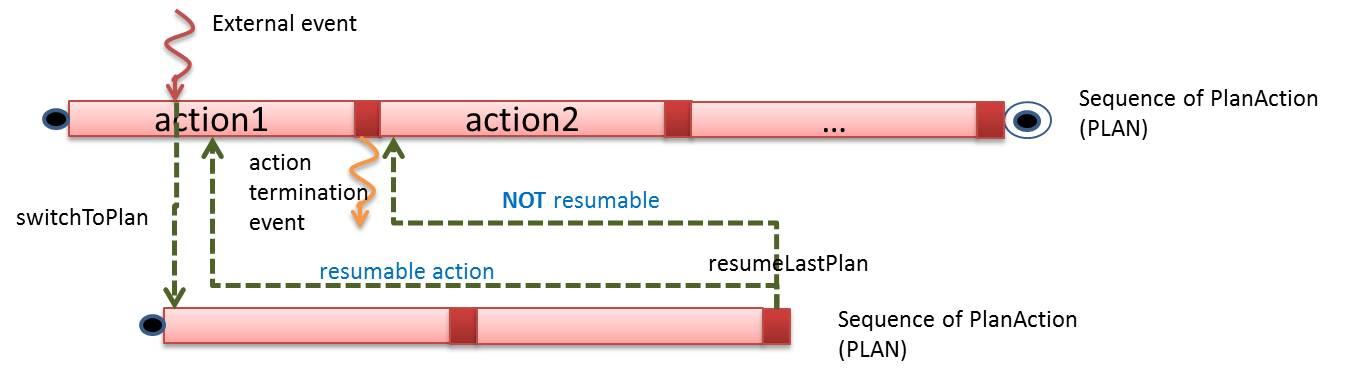
\includegraphics[scale = 0.45]{img/actionEvents.jpg}\\
\end{tabular}{   }
\end{center}

\subsection{Messages and message-driven/message based behaviour} 
\labelssec{defmessages}
A \textbf{\textit{message}} is defined here as information sent in \textit{\textbf{asynchronous}} way by some source to some specific destination. For  \textit{asynchronous} transmission we intend that the messages can be 'buffered' by the infrastructure, while the  'unbuffered' transmission is said to be \textit{\textbf{synchronous}}.

Messages can be \textit{\textbf{sent}} and/or \textit{\textbf{received}} by the \textit{QActors} that compose a \textit{qactor-system}. A message does not force the execution of code: it can be managed only after the execution of an explicit \textit{receive} action performed by a  \textit{QActor}. Thus we talk of \textit{massage-based} behaviour only, by excluding \textit{massage-driven} behaviour (the default behaviour in \akka).

Messages are represented as follows:

\begin{qacode}
msg( MSGID, MSGTYPE, SENDER, RECEIVER, CONTENT, SEQNUM )
\end{qacode}

where\footnote{At the moment only \texttt{dispatch}, \texttt{request} and \texttt{event} are implemented}  :
\medskip 
\texttt{
\begin{tabular}{|l|l|}
\hline 
MSGID	& Message identifier \\ 
\hline 
MSGTYPE	& Message type (e.g.:dispatch,request,invitation,event,token) \\ 
\hline 
SENDER	 & Identifier of the sender  \\ 
\hline 
RECEIVER	& Identifier of the receiver \\ 
\hline 
CONTENT	 & Message payload \\ 
\hline 
SEQNUM	 & Unique natural number associated to the message \\ 
\hline 
\end{tabular} 
}

The \texttt{msg/6} pattern can be used to express \textit{guards} (see \xss{guardedaction}) to allow conditional evaluation of \textit{PlanActions}.

\subsection{Events and event-driven/event-based behaviour } 
\labelssec{defevents}
 
An \textbf{\textit{event}} is defined here as information emitted by some source without any explicit destination. Events can be \textit{\textbf{emitted}} by the \textit{QActors} that compose a \textit{actor-system} or by sources external to the system.

The occurrence of an event can put in execution some code devoted to the management of that event. We qualify this kind of behaviour as \textit{\textbf{event-driven}} behaviour, since the event 'forces' the execution of code (see \xss{evenHandler}).

An event can also trigger state transitions in components, usually working as finite state machines that call operations to explicitly \textit{\textbf{sense}} events (see \xss{senseaction}). We qualify this kind of behaviour as \textit{\textbf{event-based}} behaviour, since the event is 'lost' if no actor is in a state waiting for it.

Events are represented as messages (see \xss{defmessages}) with no destination (\texttt{RECEIVER=none}):

\begin{qacode}
msg( MSGID, event, EMITTER, none, CONTENT, SEQNUM )
\end{qacode}

 

\subsection{Actor programs as plans}
\labelssec{actorplans}
 
A \textit{\textbf{qactor-program}} consists in a set of \textit{Plans}; the (unique, mandatory) \textit{Plan} qualified as \texttt{normal} is executed as the actor main activity. Other plans can be put in execution by the main plan according to action-based, event-based or message-based behaviour.

Each plan has a name and can be put into execution by a proper \textit{PlanAction} (including an explicit \texttt{switchToPlan}, see \xss{basicactions}). Plans can be stored in files and dynamically loaded by the user into the \textit{actor-mind} (see \xss{}).

A plan is represented in files as a sequence of 'facts', each expressed in the following way:
\begin{Verbatim} [fontsize=\scriptsize, frame=single, label=Internal representation of plans]		
plan(ACTIONCOUNTER,PLANNAME,sentence(GUARD,MOVE,EVENTLIST,PLANLIST))
\end{Verbatim} 
For example:

\begin{Verbatim} [fontsize=\scriptsize, frame=single, label=Internal representation of a plan]		
plan(0,p0,sentence(true,move(playsound,'./audio/tada2.wav',1500),'',''))
plan(1,p0,sentence(true,move(playsound,'./audio/music_interlude20.wav',20000),
	                                     'usercmd,alarm','handleUsercmd,handleAlarm'))
\end{Verbatim} 

This internal representation of Plans can be the input of a run-time \textit{PlanInterpreter} that can execute plans dynamically created by the actor. This can be a support for experiments in the field of \textit{automated planning}.

\subsubsection{Actor programs as finite state machines (FSM)}.\\
\labelssec{progasfsm}

A \textit{Plan} can be viewed as the specification of a \textbf{state} of a \textit{finite state machine} (\texttt{FSM}) of the Moore's type  and should \textbf{not} be interpreted as a procedure. In fact a plan can be put in execution by events (see \xss{defevents}) and returns the control to the 'calling' plan only when it executes (as last action) a '\texttt{resumeLastPlan}'  (otherwise the computation ends). 

\begin{center}
\begin{tabular}{ c }
     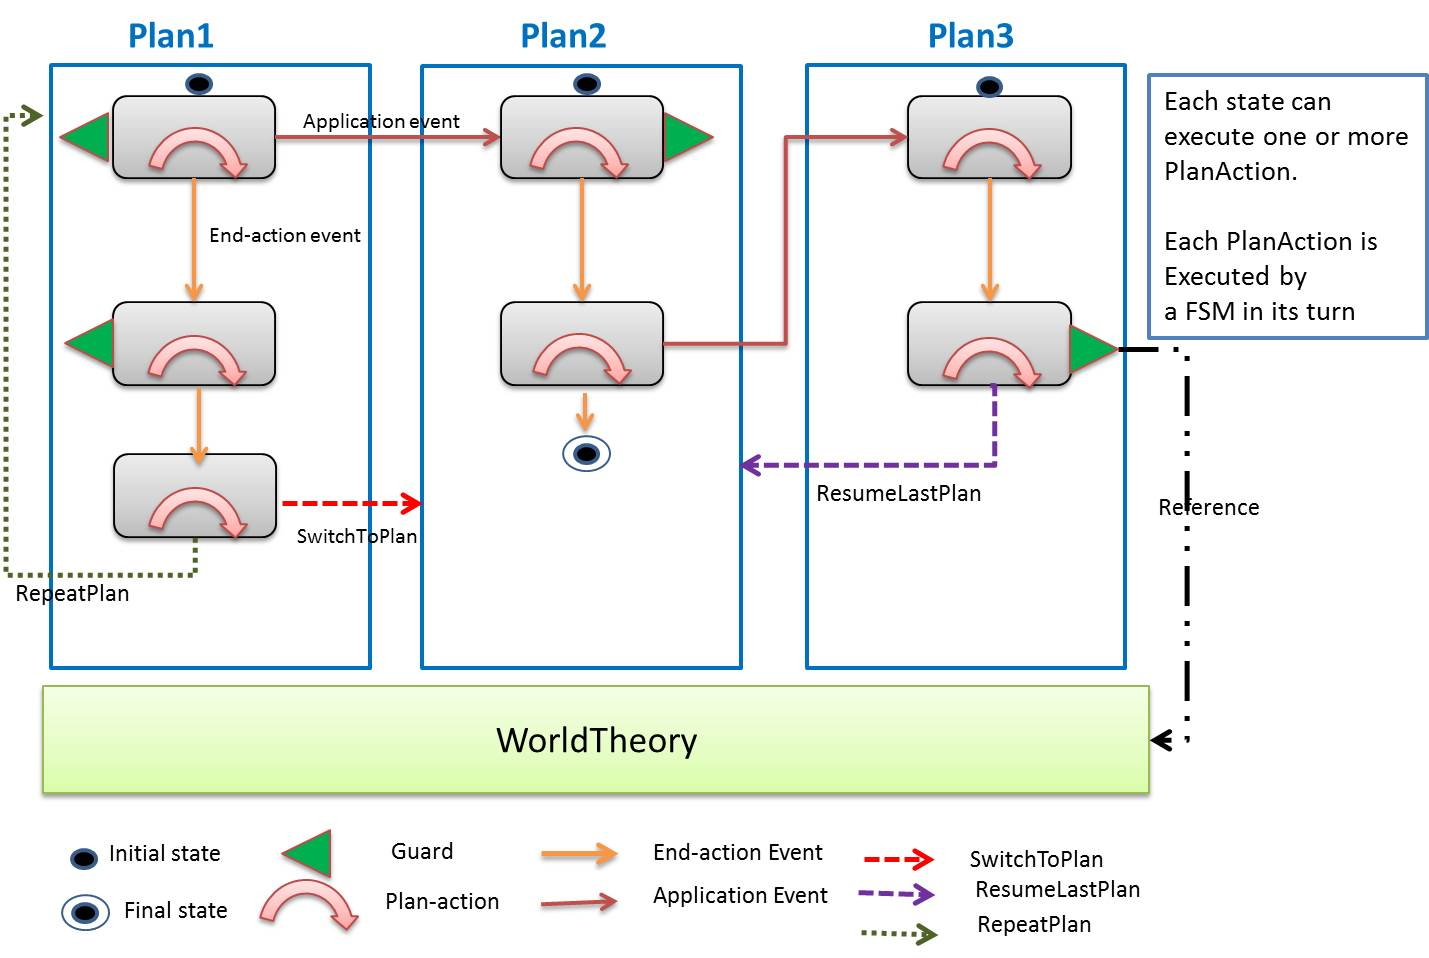
\includegraphics[scale = 0.55]{img/planFSM.jpg}\\
\end{tabular}{   }
\end{center}

State transitions are usually caused by messages or events but that can be caused also by explicit built-in actions such as \texttt{switchToPlan}.

A timed \textit{PlanAction} is in its turn implemented as \texttt{FSM} that can generate different kinds of termination events:
\begin{itemize}
\item a (built-in) normal termination event;
\item a user-defined termination event (see \xss{asynchaction});
\item a time-out termination event;
\item a abnormal termination event;
\end{itemize}

%%Examples of plans are given in \xs{aseqplans}.

\newpage 
\section{The \texttt{qa} language/metamodel.}
\labelsec{introqa}

The \textit{qactor} (\texttt{qa}) language is a custom language built by exploiting the \xtext{} technology\footnote{The \texttt{qa} language/metamodel is defined in the project \textit{it.unibo.xtext.qactor}.}; thus, it is also a meta-model. Technically we can say that \texttt{qa} is a 'brother' of \texttt{UML} since it is based on \texttt{EMOF}.

The language-metamodel \texttt{qa} aims at overcoming the \textit{abstraction gap} between the needs of distributed \textit{proactive/reactive} systems and the conventional (object-based) programming language used for implementation (mainly \texttt{Java, C\#, C}, etc).
In fact, a \texttt{qa} specification aims at capturing main \textit{architectural} aspects of the system by providing a support for \textit{rapid software prototyping}.

%%that has been defined to proved models as \textit{executable specifications} of distributed software systems according to three main dimensions: \textit{structure}, \textit{interaction} and \textit{behaviour}.

%%%%% \subsection{Example}
%%%%% \labelssec{qaexample}

%%%%% As an example of \textbf{qa} specifications, we define the behaviour of an actor as a \qa{} able to execute two plans: an initial \texttt{init} plan (qualified as '\texttt{normal}') that calls another plan named \texttt{playMusic} that, once terminated, returns the control to the previous one:

%%%%% %%\footnote{A \textbf{\textit{mock}} actor is a 'virtual' entity that simulates movements and sensors.}
%%%%% \lstinputlisting[language=qa,caption={ \texttt{basic.qa} }, firstline=1 ]{../../../it.unibo.qactors.tests/src/basic.qa}  
 
%%%%% %% \subsection{Qactor as a QActor, component of a distributed system}
%%%%% %% \labelssec{distrqactor}

%%%%% The \textbf{qa} specification shows that a \textit{Qactor} is an element of a distributed software system (\textit{qactor-system} from now-on); the actor can work in cooperation/competition with other actors and other components, each modelled as a \textit{QActor}.

Each \textit{Qactor} is able to execute a set of built-in actions to send/receive messages and to emit/sense events. This section is devoted to a brief introduction to the language rules that define the syntax of these operations.
 



\subsection{Messages and message based behaviour} 
\labelssec{intromessages}
A \qa{} can \texttt{send}/\texttt{receive} \textit{\textbf{messages}} to/from another \textit{Qactor} working in the same or in another \textit{Context}. A \qa{} can also send messages to itself.

The \texttt{qa} language allows us to express \texttt{send/receive} actions as high-level operations that hide at application level the details of the communication support. The \qa{} software factory generates the code required to exploit the \qa{} run time support to implement the message-passing operations. 

The \texttt{qa} language defines the following syntax for message declaration: 

\begin{javacode}
Message :     	    OutOnlyMessage | OutInMessage  ;
OutOnlyMessage : 	Dispatch |  Event | Signal | Token ; 
OutInMessage: 		Request  | Invitation ;

Event: 		"Event"      name=ID  ":" msg = PHead  ;
Signal: 	"Signal"     name=ID  ":" msg = PHead  ;
Token:		"Token"      name=ID  ":" msg = PHead  ;
Dispatch: 	"Dispatch"   name=ID  ":" msg = PHead  ;
Request: 	"Request"    name=ID  ":" msg = PHead  ;
Invitation:	"Invitation" name=ID  ":" msg = PHead  ;
\end{javacode}
 
%%\subsubsection{PHead.}

\textbf{\textit{PHead}}:
The  \texttt{PHead}  syntax rule defines a subset of \prolog{}  syntax:
\labelssec{phead}

\begin{javacode}
	PHead : PAtom | PStruct ;
	PAtom : PAtomString | Variable | PAtomNum | PAtomic  ;
	PStruct : name = ID "(" (msgArg += PTerm)? ("," msgArg += PTerm)* ")"; 
	PTerm   : PAtom | PStruct ...
\end{javacode}
 
\subsection{Send actions}
At \texttt{qa} level, high-level forms of sending-message actions are defined:

\begin{itemize}
\item forward a dispatch
\item demand a request
\item ask an invitation
\item ...
\end{itemize}

%%\noindent \textbf{Operation that sends a \textit{dispatch}}  
\subsubsection{Forward a \textit{dispatch}: syntax}.
\medskip 
\begin{javacode}
SendDispatch: name="forward" dest=VarOrQactor "-m" msgref=[Message] ":" val = PHead ;
VarOrQactor : var=Variable  | dest=[QActor] ;
\end{javacode}

\noindent Example:
\begin{Verbatim}[fontsize=\scriptsize, frame=single]
forward receiver -m info : info(a)  
\end{Verbatim}	


%%\noindent \textbf{Operation that sends a a \textit{request}} 
\subsubsection{Demand a \textit{request}: syntax}. 
\medskip 
\begin{javacode}
SendRequest: name="demand" dest=VarOrQactor "-m" msgref=[Message] ":" val = PHead  ;
\end{javacode}


\noindent Example:
\begin{Verbatim}[fontsize=\scriptsize, frame=single]
demand receiver -m eval : fibo(25,V)   
\end{Verbatim}

 
\subsection{Receive actions}
 
The \texttt{qa} language defines several forms of high-level receive-message actions  : 

\begin{itemize}
\item receive any message
\item receive a message with optional message specification
\item receive a message with a specific structure
\end{itemize}

%\noindent \textbf{Generic receive with optional specification} 
\subsubsection{Generic receive with optional message specification: syntax}.
\begin{javacode}  
ReceiveMsg : name="receiveMsg" duration=TimeLimit (spec=MsgSpec)? ;
	TimeLimit : name="time" "(" ( msec=INT | var=Variable ) ")" ;
	MsgSpec   : "-m" msg=[Message]  "sender" sender=VarOrAtomic "content" content=PHead ; 
\end{javacode}

\noindent Example1: receive a message
\begin{Verbatim}[fontsize=\scriptsize, frame=single]
receiveMsg time( 1000 )   
\end{Verbatim}	

\noindent Example2: receive a message  from a specific \texttt{sender} with some specific payload structure:
 \begin{Verbatim}[fontsize=\scriptsize, frame=single]
receiveMsg time(100) -m info sender ansa content news(sport(X)) 
\end{Verbatim}

%\noindent \textbf{Receive a message with a specified structure} 
\subsubsection{Receive a message with a specified structure: syntax}.
 
\begin{javacode}  
OnReceiveMsg: name="receiveTheMsg" "m" "(" msgid=PHead ","   msgtype=PHead "," msgsender=PHead 
 	"," msgreceiver=PHead "," msgcontent=PHead "," msgseqnum=PHead ")" duration=TimeLimit  ;
\end{javacode}

\noindent Example: receive the message whose internal structure \texttt{msg/6} is unifiable with the given arguments:
\begin{Verbatim}  [fontsize=\scriptsize, frame=single]
receiveTheMsg m( info,dispatch,ansa,R,news(sport(X)),N) time(2000) 
\end{Verbatim}

Once a message has been received, the \texttt{onMsg} action allows us to select a message and execute actions according to the specific structure of that message. 

%\noindent \textbf{Select a message and execute} 
\subsubsection{onMsg: syntax}.
\begin{javacode}  
MsgSwitch : "onMsg" message=[Message]   ":" msg = PHead "->" move = Move;
Move      : ActionMove | MessageMove | ExtensionMove  | BasicMove | PlanMove | GuardMove | BasicactorMove;
\end{javacode}

\noindent Example: print (part of the) content of a message 
\begin{Verbatim}[fontsize=\scriptsize, frame=single]
//some receive ...
onMsg info :  news(sport(X))} -> println(X)
\end{Verbatim}
 


 
\subsection{Events and event-based behaviour } 
\labelssec{introevents}


\textit{QActors} can \texttt{emit} and \texttt{sense} (perceive) \textit{events	} represented as follows:

\begin{qacode}
msg( MSGID, event, SENDER, none, CONTENT, SEQNUM )
\end{qacode}

 
\subsubsection{Emit an event: syntax}.

The \texttt{qa} language defines an high-level action to emit events
 
\begin{javacode}  
 RaiseEvent : name="emit" ev=[Event] ":" content=PHead  ;
\end{javacode}
	
\noindent Example 
\begin{Verbatim}[fontsize=\scriptsize, frame=single]
emit alarm : alarm(fire)
\end{Verbatim}

 


 
\subsubsection{Sense events: syntax}.\\
\labelssec{senseaction}
To allow \textit{\textbf{event-based}} behaviour, \texttt{qa} provides a \textit{\textbf{sense}} operation that blocks the execution of a \qa{} until the required event occurs. 

 
 
\begin{javacode}  
SenseEvent : "sense" duration=TimeLimit events += [Event] ("," events += [Event] )*  
		"->" plans += Continuation ("," plans += Continuation )* ; 
Continuation: plan = [Plan] |  name="continue"  ;
\end{javacode}
 

\noindent Example
\begin{Verbatim}[fontsize=\scriptsize, frame=single]
sense time(1000) alarm -> continue
\end{Verbatim}


 
\subsubsection{OnEvent action: syntax }
The \texttt{qa} language defines also an event-selection  action: 
 
\begin{javacode}  
EventSwitch : "onEvent" event=[Event]  ":" msg = PHead "->" move = Move  ;
\end{javacode}

\noindent Example 
\medskip 
\begin{Verbatim}[fontsize=\scriptsize, frame=single]
//sense ...
onEvent alarm :  alarm(fire} -> sound time(2500) file( "./audio/illogical_most2.wav") 
\end{Verbatim}	

\subsection{Event handlers and event-driven behaviour }
\labelssec{evenHandler}
The occurrence of an event activates, in \textit{\textbf{event-driven}} way, all the \textbf{\textit{EventHandlers}} 'registered' (i.e.declared in some \textit{Context}) for that event. 
%%The \textit{EventHandlers} are activated one at the time by a single-thread scheduler. 
  
In the \texttt{qa} language, the declaration of an \textit{EventHandler} must be done within a \textit{Context} with the following syntax: 

\begin{javacode}  
EventHandler :  
 	"EventHandler" name=ID   ( "for" events += [Event] ( "," events += [Event] )* )? 
 	( print ?= "-print") ?
 	( "{"  body = EventHandlerBody "}" )?
 	";" 
EventHandlerBody:
	 op += EventHandlerOperation (";" op += EventHandlerOperation)* 
;
EventHandlerOperation:
	MemoOperation | SolveOperation | RaiseEvent | SendEventAsDispatch
;
MemoOperation:
	"memo" rule=MemoRule "for" actor=[QActor]
	| doMemo=MemoCurrentEvent "for" actor=[QActor]
;
SolveOperation:
	"solve" goal=PTerm "for" actor=[QActor]
;
SendEventAsDispatch :
	"forwardEvent" actor=[QActor] "-m" msgref=[Message]
; 
MemoRule :
	MemoEvent //  | Others memo rules
;
MemoEvent :
	name="currentEvent"
; 	
\end{javacode}

The syntax shows that, in a \texttt{qa} model, we can express only a limited set of actions within an EventHandler\footnote{Of course, other actions can be defined directly in \java{} by the Application designer.}:

\begin{itemize}
\item memorize and event into the WorldThery of a specific \qa{}
\item solve a goal
\item forward a dispatch with the content of the event
\item emit another event
\end{itemize}

In the example that follows, the system reacts to all the events by storing them in the knowledge base (\textit{WorldTheory}) related to a event tracer actor, that periodically shows the events available.

\lstinputlisting[language=qa,caption={ \texttt{eventTracer.qa} }, firstline=1 ]{../../../it.unibo.qactors.tests/src/eventTracer.qa}  


\subsection{Guarded actions}
\labelssec{guardedaction}

Actions prefixed by a \texttt{[ GUARD ]} are executed only when the \texttt{GUARD} is evaluated \texttt{true}. In the \texttt{qa} language, the \texttt{GUARD} is a boolean condition expressed as a \prolog{} term that can include unbound variables, possibly bound during the guard evaluation phase.
Moreover:

\begin{itemize}
\item  the prefix \texttt{\textbf{!?}} before the guard condition means that the knowledge (\prolog{} fact or rule) that makes the guard \texttt{true} must \textit{\textbf{not}} be removed form the actor's \textit{WorldTheory};
\item the prefix \texttt{\textbf{??}} means that the \prolog{} fact or rule that makes the guard \texttt{true} must be removed from  the actor's \textit{WorldTheory}.
\end{itemize}

For example;
\lstinputlisting[language=qa,caption={ \texttt{actionGuarded.qa} }, firstline=1 ]{../../../it.unibo.qactors.tests/src/actionGuarded.qa}  

Note that the \texttt{msg/6} structure is used as guard.

\subsection{About implementation}  
\labelssec{introctx}
  

Each \textit{Qactor} must work within a  \texttt{Context} that models a computational node associated with a network \texttt{IP} (\texttt{host}) and a communication \texttt{port}. 

From a model written in the \qa{} language, the \qa{} software factory generates the internal (\akka) actors that allow 
messages exchanged among \qa{} working on different contexts to flow throw the context ports (using the \texttt{TCP/IP} protocol) and to deliver the message in the message-queue of the destination \qa{}.
 
\begin{center}
\begin{tabular}{ c }
     \includegraphics[scale = 0.35]{../../../it.unibo.iss2015intro/docs/Frameworks/qactor.jpg}\\
\end{tabular}{   }
\end{center}
\subsubsection{Sending messages}.\\
\labelssec{sendImpl}
Messages can be sent to a \textit{Qactor} by using the built-in basic \texttt{sendMsg} asynchronous, point-to-point action. The \texttt{API} provided by the \texttt{qa} run-time support\footnote{The \texttt{qa} run-time support is stored in \textit{qa18Akka.jar}} has the following signature:

\begin{javacode}
void sendMsg( String msgID, String destActorId, String msgType, String content ) throws Exception
\end{javacode} 

\subsubsection{Receiving messages}.\\
The \texttt{qa} run-time support provides the following operation:
\begin{javacode}
AsynchActionResult receiveMsg( String msgid, String msgtype, String msgsender, String msgreceiver, 
			String msgcontent, String msgseqnum, int timeout, String events, String plans ) throws Exception
\end{javacode}

\texttt{AsynchActionResult} stores the results of the operation (see \xss{AsynchActionResult}).

The \texttt{receiveMsg} operation blocks the execution until a messages is received or the specified \texttt{timeout} expires. The message must \textbf{\textit{unify}} (with \prolog{} semantics) with the given arguments.
 
The \texttt{receiveMsg}  operation is 'reactive' to the specified \textit{events}. i.e. it transfers the control to the corresponding plan in \textit{plans} when one of the specified events occurs while the operation is still waiting for messages. Thus  \texttt{receiveMsg} is not a simple procedure, but it is executed by a proper \textit{Finite State Machine}.

%%\noindent It is implemented as follows (see \xss{sendImpl}):
\subsubsection{forward implementation (see \xss{sendImpl})}.
\begin{javacode}
void forward(String msgId, String dest, String msg) throws Exception{sendMsg(msgId,dest,"dispatch",msg ){
	sendMsg(msgId, dest, QActorContext.dispatch, msg)
}
\end{javacode} 

%\noindent It is implemented as follows (see \xss{sendImpl}):
\subsubsection{demand implementation (see \xss{sendImpl})}.  
\begin{javacode}
void demand(String msgId, String dest, String msg) throws Exception{sendMsg(msgId,dest,"request",msg){
	sendMsg(msgId, dest, QActorContext.request, msg);
}
\end{javacode}

\subsubsection{emit implementation}.
The \texttt{qa} run-time support provides the following operations:
\begin{javacode}
void emit( String evId, String evContent ) throws Exception
\end{javacode}

\subsubsection{sense implementation}.
The \texttt{qa} run-time support does introduce the following operation:

\begin{javacode}
AsynchActionResult senseEvents(int tout, String events, String plans, 
		String  alarmEvents, String recoveryPlans, ActionExecMode mode) throws Exception{
\end{javacode}

\subsection{QActor knowledge}
\labelssec{qaknowledge}
The picture hereunder shows that each actor is associated to a set of tuProlog theories:
\begin{center}
\begin{tabular}{ c }
     \includegraphics[scale = 0.5]{../../../it.unibo.iss2015intro/docs/Frameworks/img/qactors0.jpg}
\end{tabular}{   }
\end{center}

\begin{itemize}
\item A theory (\texttt{systemConfig.pl}) that describes the configuration of the system.
\item A theory \texttt{sysRules.pl} that describes a set of rules used at system configuration time.
\item A theory \texttt{WorldTheory.pl} that describes a set of rules and facts that give a symbolic representation of the "world" in which a \qa{} is working.
\end{itemize}

Let us report here some common functional actions (implemented by the \textit{WorldTheory} associated with each actor) that we can ask a QActor to do.


\subsubsection{Inspect the state and elaborate in a functional way}.\\
\medskip
\noindent
\begin{footnotesize}
\begin{tabular}{|p{0.5\textwidth}|p{0.5\textwidth}|}
\hline 
\texttt{ actorPrintln(hello) } & prints hello \\ 
\hline 
\texttt{ actorobj(A) } & binds A to the name of current actor (robot)  \\ 
\hline 
\texttt{ goalResult(A) } & binds A to the result of last \prolog{} goal solved by the actor \\ 
\hline 
\texttt{ result(A) } & binds A to the result of last action executed by the actor \\ 
\hline 
\texttt{ fib(10,V),result(A),actorPrintln(r(A)) } & prints \texttt{r(fib(10,89))} \\ 
\hline 
\texttt{ fib(5,V),goalResult(GR),actorPrintln(r(GR)) } & prints \texttt{r(executeInput(do([true],fib(10,89),...))} \\ 
\hline 
\end{tabular} 
\end{footnotesize}

\subsubsection{Change the internal state}.\\

The \textit{WorldTheory} associated with a robot defines also rules that allows an application designer to bind symbols to values and to add/remove rules:

\medskip 
\noindent
\begin{footnotesize}
\begin{tabular}{|p{0.5\textwidth}|p{0.5\textwidth}|}
\hline 
\texttt{ assign(x,3)} & set \texttt{x=3}, i.e. store the fact: \texttt{ value(x,3)} \\ 
\hline 
\texttt{ getVal(x,V)} & binds \texttt{V} with the current value of x \\ 
\hline 
\texttt{ assign(ledstate,false)} & set fact: \texttt{ value(ledstate,false)} \\ 
\hline 
\texttt{ inc(x,1,V) } & binds V to the result of \texttt{x+1}.  \\ 
\hline 
\texttt{ assign(x,1),inc(x,3,V),actorPrintln(v(V))} & binds V to 4 and prints \texttt{v(4)}.  \\ 
\hline 
\texttt{ assign(x,10),getVal(x,VX),actorPrintln(x(VX))} & prints \texttt{x(10)}.  \\ 
\hline 
\texttt{ addRule(r1(a)),r1(X),actorPrintln(X) } & add the fact \texttt{r1/1} to the actor's WorldTheory and  prints \texttt{a} \\ 
\hline 
\end{tabular} 
\end{footnotesize}
\newpage 
\section{Human interaction with a Qactor}
\labelsec{humaninteraction}

A human user can interact with a \qa{} by using both a remote and a local GUI interface.

\subsection{The (remote) Web interface}

\begin{center}
\begin{tabular}{ |p{0.5\textwidth}|p{0.5\textwidth}| }
\hline 
\raisebox{-\totalheight}{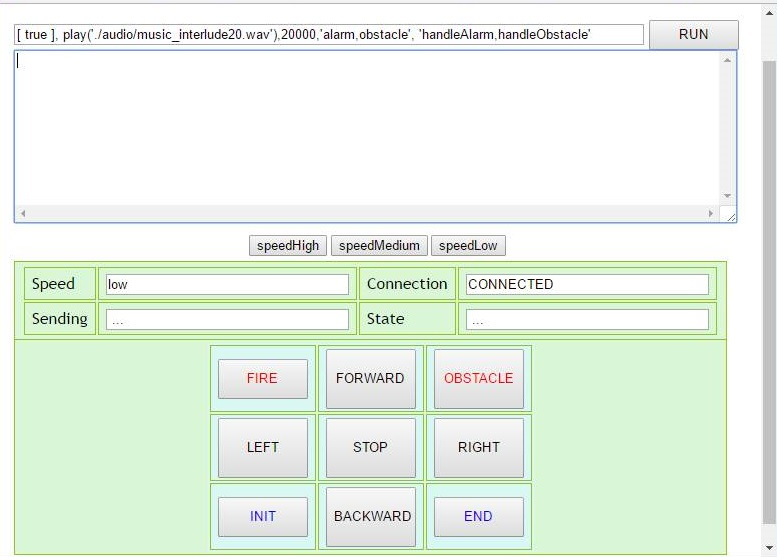
\includegraphics[width=0.5\textwidth, height=60mm]{img/guiweb.jpg}}
&
\begin{footnotesize}
     This web interface is automatically generated in the \texttt{srcMore} directory in a package associated with each \textit{Context} when the \texttt{-httpserver} flag for a Context is set. It is implemented by a \texttt{HTTP} web-socket server working on port \texttt{8080}.
     
\medskip
The \texttt{RUN} button at the top of the GUI allow us to ask the robot to execute actions, while the buttons at the bottom allows us to move the (basic) robot and send alarms.

\medskip 
The top-level part of the GUI can be used to inspect and change the state of the robot as represented in the robot's WorldTheory.     
\end{footnotesize}
\\
\hline  
\end{tabular} 
\end{center}

This interface emits the following events:  

\begin{center}
\begin{tabular}{ |p{0.7\textwidth}|p{0.3\textwidth}| }
\hline
\texttt{inputcmd  : usercmd(executeInput(CMD))} &	(\texttt{RUN} button)   \\
%%\texttt{usercmd : usercmd(robotgui(MOVE))}, \texttt{MOVE=w(low),...,s(high)} & (\texttt{MOVE} button) \\ 
\texttt{usercmd   : usercmd(robotgui(w(low)))}   &	(\texttt{FORWARD} button) \\
\texttt{alarm     : alarm(fire)}  	&	(\texttt{FIRE} button)  \\ 
\texttt{obstacle  : obstacle(X)}    	&	(\texttt{OBSTACLE} button) \\
\texttt{cmd       : cmd(start)}  	&	(\texttt{START} button)  \\ 
\texttt{cmd       : cmd(stop)}  	&	(\texttt{STOP} button)  \\ 
\hline  
\end{tabular} 
\end{center}
  
 
\subsection{The (local) GUI user interface}

\begin{center}
\begin{tabular}{ |p{0.5\textwidth}|p{0.5\textwidth}| }
\hline 
\raisebox{-\totalheight}{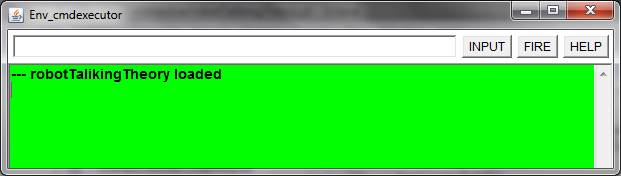
\includegraphics[width=0.5\textwidth]{img/guijava.jpg}}
     &
\begin{footnotesize} 
This interface is automatically generated as part of the(Abstract)  actor class  when the \texttt{-g} flag for an Actor is set.    

The \texttt{INPUT} button generates the event :

\medskip 
     \texttt{ local\_inputcmd : usercmd(executeInput(CMD))}	

\medskip       
where \texttt{CMD} is the content of the input field on the left.
\end{footnotesize}
\\
\hline      
\end{tabular} 
\end{center}
 
In \xs{aboutactions} we will introduce an interpreter allowing human users to execute actions expressed as commands using a Web or a GUI actor interface.



\section{Building qa models}
\labelssec{qaworkflw}

A goal of  \texttt{qa} is  to help software developers in writing \textit{executable specifications} during the early stages of software development with particular regard to \textit{requirement analysis} and \textit{problem analysis}. More precisely, the main outcome of the problem analysis phase should be the specification of the \textit{logical architecture} of the system, obtained by following a sequence of steps:

\begin{itemize}
	\item find the main subsystems and define the system \textit{Contexts};
	\item define the structure of the \textit{Events} that can occur in the system;
	\item define the structure of the \textit{Messages} exchanged by the actors;
	\item define the main \textit{Actors} working in each \textit{Context};
	\item define the type of the \textit{logical interaction} among the actors;
	\item define the \textit{logical behaviour} of each actor according to the interaction constraints.
\end{itemize}

In several cases these specifications can be refined in the \textit{project phase} by simply 'injecting' application-specific actions (see \xs{useraction}) so to reduce the global costs of software development.

\subsubsection{Application designer and System designer.}

In the following, we will name  \textit{application designer} the software designer that works to fulfil the functional requirements of system while we will name  \textit{system designer} the designer that provides the run-time supports useful to face the business logic without too much involvement in technical problems related to distribution or to other relevant, recurrent, general problems in the application domain.



\subsection{QActor software factory} 

\qa{} systems run upon a run-time support  (built in the project \textit{it.unibo.qactors}) based on the \akka{} actor system and is deployed (at this moment) in the 'library' \textit{qa18Akka.jar}\footnote{another library \textit{qactors17.jar} is provided for Android that does not support yet java8}. The \qa{} run-time support requires in its turn other open-source and custom libraries. 

Thanks to the Xtext technology and Eclipse, the \qa{} language/metamodel is associated to a software factory that automatically generates all the files (Prolog theories) and the proper system configuration code, so to allow Application designers to focus on application logic.


\newpage 


\newpage 
 \section{User-defined actions in \prolog}
\labelsec{useraction}
 
The user can define application-specific actions in two main ways: \textit{(i)} by using \java{} or some other (\java{}-compatible) programming language or (ii) by using \tuprolog{}.
 
In this section we will explore how the application designer can exploit \tuprolog{} in order to define business-specific operations.

\subsubsection{Examples of unification}.
Let us recall here that tuProlog does implement occur check (and variable renaming):

\begin{Verbatim} [fontsize=\scriptsize, frame=single, label=Action examples]
a(X,1)=a(1,Y)       '='(a(1,1),a(1,1))
a(X,1)=a(1,X)       '='(a(1,1),a(1,1)))
a(X,2)=a(1,X)       a(_1,_2)		//tuProlog rewrites variables (occur check)

a(b(X,1),c(Y))=a(b(0,A),c(A)) '='(a(b(0,1),c(1)),a(b(0,1),c(1))
a(b(X,1),c(Y))=Z              '='(a(b(_2,1),c(_1)),a(b(_2,1),c(_1)))
a(b(X,1),c(Y))=a(A,B)         '='(a(b(_6,1),c(_1)),a(b(_6,1),c(_1)))
\end{Verbatim}

\subsection{The \texttt{demo} and \texttt{solve} operation.}
\labelssec{solve}

The \texttt{qa} language defines actions to \texttt{solve} \prolog{} goals: 
 
\begin{itemize}
\item
\begin{javacode}  
Demo:	"demo" goal=PHead ("onFailSwitchTo" plan=[Plan])?;
SolveGoal:	"solve" goal=PHead duration=TimeLimit ("onFailSwitchTo" plan=[Plan])?;
\end{javacode}
\end{itemize}

In both cases, the result is represented by the fact \texttt{goalResult/1} in the actor \textit{WorldTheory} (see \xss{mind}). The duration of a \texttt{demo} action is set to 1 day (\texttt{86400000} msec).

\subsection{Loading and using a user-defined theory}
The \textit{WorldTheory} of an actor can be extended by the application designer by using the directive\footnote{A \tuprolog{} directive is a query immediately executed at the theory load time.} \texttt{consult}. 

For example, the following system loads (\texttt{0}) a user-defined theory (stored in file \texttt{aTheory.pl}) and then \textit{(i)}finds a Fibonacci number (plan \texttt{compute}), \textit{(ii)}works with sensor data, for two times in the same way (plan \texttt{accessdata}) :

\lstinputlisting[language=qa,caption={ \texttt{aTheoryUsage.qa} }, firstline=1 ]{../../../it.unibo.qactors.tests/src/aTheoryUsage.qa}  

The theory stored in \texttt{aTheory.pl}) includes data (facts) and rules to compute relevant data:
\lstinputlisting[language=qa,caption={ \texttt{aTheory.pl} }, firstline=1 ]{../../../it.unibo.qactors.tests/aTheory.pl}  

\subsubsection{The initialization directive.}
The following directive:
\medskip 
\begin{Verbatim}[fontsize=\scriptsize, frame=single]
:- initialization(initialize).  
\end{Verbatim}
sets a starting goal to be executed just after the theory has been consulted. 

Thus, the output of the \texttt{theoryusage} actor is:

\begin{javacode}
--- initializing the aTheory ...
--- fib(7,13)
---  "-------------------------------------" 
--- data(sonar,1,10)
--- validDistance(2,20)
--- warning(2,20)
--- nears([d(2,20),d(3,30)])
---  "-------------------------------------" 
--- data(sonar,1,10)
--- validDistance(2,20)
--- warning(2,20)
--- nears([d(2,20),d(3,30)])
--- bye
\end{javacode}

\subsubsection{On backtracking.}
The output shows that the rules \texttt{validDistance and nearDistance} exploit \textit{backtracking} in order to return the first valid instance (\texttt{2}), while the repetition of the plan \textit{accessdata} returns always the same data\footnote{Remember from \xss{worldtthfacts} that the fact goalResult/1 is a 'singleton'.}. In fact, \textit{backtracking} is a peculiarity of \prolog{} and is not included in the computational model of \qa{}. However, an actor could access to different data at each plan iteration, by performing a proper query in which  the second argument of \texttt{data/3} is used as an index (for an example, see \xss{accessData}).

\subsection{Using the actor in \prolog{} rules }
\labelssec{actorobj}

%\subsubsection{Referencing the current actor(actor).}
%\labelssec{actorobj}

The predefined rule \texttt{actorobj/1} unifies a given variable to a reference to the \java{} object that implements the actor associated with the current  \textit{WorldTheory}. In this way the application designer can access in \prolog{} to all the public methods of the actor. 

%% The \texttt{createPojoButton/4} rule binds (by using the predefined rule \texttt{actorobj/1} ) the variable \texttt{Actor} to a reference to the \java{} object that implements the actor \texttt{buttonobserver}. In this way the application designer can access in \prolog{} to all the public methods of the actor.  In our specific case, the rule gets the actor's standard output device (\texttt{OutView}) and then delegates the creation of the button  to a static method of the  \java{} class \texttt{DeviceButtonArduinoQa}


For example, the following theory defines a rule (\texttt{dance}) to (simulate a) moves of the actor in some planned way:
\lstinputlisting[language=qa,caption={ \texttt{actorDanceTheory.pl} }, firstline=1 ]{../../../it.unibo.qactors.tests/actorDanceTheory.pl}  
 
The application designer can use the \texttt{dance} rule as a user-defined extension of the actor action-set:
\lstinputlisting[language=qa,caption={ \texttt{dancer.qa} }, firstline=1 ]{../../../it.unibo.qactors.tests/src/dancer.qa}  


\subsection{The operator actorOp}
\labelssec{actorOp}
The \texttt{qa} operator \texttt{actorOp} allows us to put in execution a \java{} method written by the application designer as an application-specific part. 

Here is an example that shows how execute methods that return primitive data and methods that return objects:
\lstinputlisting[language=qa,caption={ \texttt{actorOpdemo.qa} }, firstline=1 ]{../../../it.unibo.qactors.tests/src/actorOpdemo.qa} 

The code written by the application designer is:
\lstinputlisting[language=qa,caption={ \texttt{Qaactorop.java} }, firstline=1 ]{../../../it.unibo.qactors.tests/src/it/unibo/qaactorop/Qaactorop.java} 

\subsection{Rules at model level}
\labelssec{rulesinmodel}
Sometimes can be useful to express \prolog{} facts directly in the model specification, especially when these facts are used for configuration or action-selection purposes. The \texttt{Rules} option within a \qa{} allows us to define facts by using a subset of the \prolog{} syntax\footnote{The extension of this option with full \prolog{} syntax is a work to do.}  

For example, let us define the model of a system that plays some vocal message on a background music by consulting its  'sound knowledge-base' defined in the \texttt{Rules} section:

\lstinputlisting[language=qa,caption={ \texttt{rulesInModel.qa} }, firstline=1 ]{../../../it.unibo.qactors.tests/src/rulesInModel.qa}  


\subsection{From \prolog{} to \java{} again}
\labelssec{javafromprolog}
Thanks to \tuprolog{} features, the application designer can define rules that can exploit \java{} to perform the required operation. For example, suppose that we have to solve to following problem:

\medskip 
\scriptsize
\framebox[15cm]{ %
\begin{minipage}{140mm}
Build a system that starts by playing a soft music in background. Then the system shows to the user a graphical interface to allow the selection of a sound file (\texttt{wav}). When the user has selected a file, the  graphical interface disappears and the system plays the selected (short) sound over the music in background.
\end{minipage}}
\normalsize
\medskip    

The application designer can define a \textit{project model} like the following one:

\lstinputlisting[language=qa,caption={ \texttt{userSelect.qa} }, firstline=1 ]{../../../it.unibo.qactors.tests/src/userSelect.qa}  

\subsubsection{Guards as problem-solving operation.}
In the plan \texttt{playMusic} above, let us consider the sentence:
\begin{Verbatim} [fontsize=\scriptsize, frame=single ]	
[ !? select(FILE) ] sound time(3000) file(FILE) ;
\end{Verbatim}
When the guard evaluates to \texttt{true}, it should bind (the variable) \texttt{FILE} to the file-path selected by the user. 

\subsubsection{The user-defined \texttt{select/1} operation.}
To allow the \texttt{select/1} guard to become part of the problem-solution rather than just a test\footnote{Of course the application designer must assure that a guard computation always terminates and should avoid to write computationally heavy guards.} , the application designer writes a proper rule in the \tuprolog{} file \texttt{userTheory.pl} loaded into the actor's knowledge base by the \texttt{init} plan (at \texttt{(1)}).

\lstinputlisting[language=java,caption={ \texttt{userTheory.pl} }, firstline=1 ]{../../../it.unibo.qactors.tests/userTheory.pl}

In this example the problem can be in large part solved by making reference to objects provided by the standard \java{} library. The class \textit{it.unibo.utils.Utils} is introduced to solve in \java{} (rather than in \prolog{}) a string-substitution problem.

In fact, the \texttt{select/1} rule first creates an instance of the \java{} class \textit{javax.swing.JFileChooser} to show a dialog window to the user. Afterwards, it uses the instance referred by the variable \texttt{Dialog} to bind the  \texttt{File} variable to the file selected by the user  and then it uses the object referenced by \texttt{File} to bind  \texttt{Path} to a file-path string.
Finally, the rule calls the \textit{static} method \texttt{adjust(String path)} of the user-defined class \textit{it.unibo.utils.Utils} to replace all the backslashes with "\texttt{/}".

\lstinputlisting[language=java,caption={ \texttt{QActorUtils.java} }, firstline=63, lastline=65 ]{../../src/it/unibo/qactors/QActorUtils.java}
 
\subsection{Workflow}
\labelssec{prologworkflw}

The definition of application actions in \tuprolog{} is particularly useful during the requirement and problem analysis, since it allows us to introduce in \textit{declarative} style \textit{executable} actions. This promotes \textit{fast prototyping} of  qactor-systems, using \tuprolog{} as a 'glue' between high-level models (expressed in \texttt{qa}) and more detailed operations written in \java. 

The workflow of \xss{qaworkflw} can be extended with the following steps:
\begin{itemize}
\item make reference to the \java{} classes that constitute the \textit{domain model} expressed as conventional (\texttt{POJO}) objects ; 
\item use the \texttt{actorOp} specification to call \java{} operations;
\item define a set of \prolog{} rules, each providing (the specification of) a new \textit{operation} to be called in some specific state (\texttt{Plan}) of the actor model.
\end{itemize}

Further examples of this approach will be given in the following.

\subsection{Examples of problem solving with \tuprolog{} }
\labelssec{moreexamples}

Let us consider the following model:

\lstinputlisting[language=qa,caption={ \texttt{theoryExanple.qa} }, firstline=1 ]{../../../it.unibo.qactors.tests/src/theoryExanple.qa}  

This model defines a set of plans, each designed to solve a different problem:

\begin{itemize}
\item \texttt{configuration}: show to the user the configuration of the system.
\item \texttt{family}: given a knowledge base over a domain (a family) find some relevant information (e.g. a son of a person or all the sons of a person).
\item \texttt{accessData}: access to sensor data represented in an index-based form by an iterative computation.
\end{itemize}

The user-defined theory (stored in file \texttt{exampleTheory.pl}) is:

\lstinputlisting[language=qa,caption={ \texttt{exampleTheory.pl} }, firstline=1 ]{../../../it.unibo.qactors.tests/exampleTheory.pl}  

We note that:
\subsubsection{configuration.}
moreexamples
To solve the \texttt{configuration} problem, the application designer loads the generated theory stored in file
 \texttt{../../../it.unibo.qactors.tests/srcMore/it/unibo/ctxTheoryExanple/theoryexanple.pl}:

\lstinputlisting[language=java,caption={ \texttt{theoryexanple.pl} }, firstline=1 ]{../../../it.unibo.qactors.tests/srcMore/it/unibo/ctxTheoryExanple/theoryexanple.pl}
 
Then the problem is completely solved (output included) by the \tuprolog{} rule \textit{showSystemConfiguration}.

This example shows that choice to represent the system configuration as a theory allows applications to dynamically inspect the system and to perform actions that could depend on such a configuration.

\subsubsection{family.}
To solve the \texttt{family} problem, the application designer does use the \texttt{solve} operation to perform queries to the family knowledge-base. The \texttt{findall/3} predicate is very useful to collect a set of solution into a list.

\subsubsection{accessData.}
\labelssec{accessData}
To solve the \texttt{family} problem, the application designer has introduced some 'imperative' programming style with the rules \texttt{assign/3} and \texttt{inc/1}. The rule \texttt{nextdata/3} is used to access a different \texttt{data} value at each iteration of plan \texttt{accessData}. The iterations terminate when the \texttt{endplan} clause is executed, i.e. when the rule (guard) \texttt{nextdata/3} fails.


\subsubsection{output.}
The output of the system execution is:
\begin{javacode}
*** ctxtheoryexanple startUserStandardInput ***
Starting the actors .... 
--- initializing the exampleTheory ...
--- 	The system is composed of the following contexts
--- context(ctxtheoryexanple,localhost,'TCP','8099')
--- 	 and  of the following actors
--- qactor(thexample,ctxtheoryexanple)
--- lot
--- [d(milcah,haran),d(yiscah,haran)]
--- data(sonar,1,10)
--- data(sonar,2,20)
--- data(sonar,3,30)
--- data(sonar,4,40)
--- no more data
--- bye
\end{javacode}

\newpage 
\section{Advanced Actions (observable, timed, reactive)}
\labelsec{actions}

In \xss{actions} we said that an \textit{\textbf{action}} is an activity that must always terminate. The effects of an action can be perceived as changes in the logical or in the physical actor environment.

Let us consider here an action that computes the \texttt{n-th} number of Fibonacci (slow, recursive version):

\begin{javacode}
	protected long fibonacci( int n ){
		if( n<0 || n==0 || n == 1 ) return 1;
		else return fibonacci(n-1) + fibonacci(n-2);
	}
\end{javacode}

Usually an action expressed in this way is executed as a procedure that keeps the control until the action is terminated. Since this a 'pure computational action', its effects can be perceived (as a result of type \texttt{long}) when the action returns the control to the caller.


\subsection{Asynchronous Observable Actions}
\labelssec{actionObservable}

Let us introduce now a new idea of an action\footnote{The growing demand for asynchronous, event-driven, parallel and scalable systems demand for new abstractions.} , with the following properties:
\begin{enumerate}
\item the action performs its work in its own thread of control;
\item the action emits an \textit{event} when terminates.
\end{enumerate}

We can define an \textit{\textbf{Observable Action}} as an asynchronous action that emits a termination event\footnote{Usually, the name of the termination event starts with the prefix "\texttt{local\_}", in order to avoid event propagation over the network.}. Moreover:
\begin{itemize}
\item the action can be activated in two different ways: synchronous mode and asynchronous mode;
\item a Observable Action activated in  \textit{synchronous} mode blocks the activator until the action is completed;
\item a Observable Action activated in  \textit{asynchronous} mode returns immediately the control to the activator;
\item the \textit{result} of a Observable Action is an object of some type \texttt{T}.
\end{itemize}

Thus, an Observable Action works in parallel with its activator that can decide to wait for the termination of the action. The action effects (results) can be perceived by means of an operation (if it is defined) that gives (when the action is terminated) the result of the action or by means of an event-driven or an event-based behaviour.

\begin{center}
\begin{tabular}{ c }
     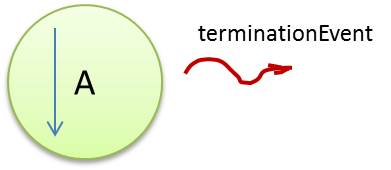
\includegraphics[scale = 0.5]{img/actionObservable.jpg}\\
\end{tabular}{   }
\end{center}
 

\subsection{The class \texttt{ActionObservableGeneric}}
\labelssec{actionObservableGeneric}

The generic, abstract class \texttt{ActionObservableGeneric<T>} provides an implementation support for Observable Actions. It implements the following interface \footnote{The code is included in the file \textit{qactor18.jar}.}  

\lstinputlisting[language=java,caption={ \texttt{IObservableActionGeneric<T>} }, firstline=1 ]{../../../it.unibo.qactors/src/it/unibo/qactors/action/IObservableActionGeneric.java}

The meaning of some important operations is reported in the following table:

\medskip 
\begin{tabular}{|l|l|}
\hline
\texttt{T execSynch()} & executes the action and waits for termination \\ 
\hline 
\texttt{Future<T> execAsynch()} & starts the action as an asynchronous operation \\ 
\hline 
\texttt{String getTerminationEventId()} & returns the name of the termination event\\ 
\hline 
\texttt{long getExecTime()} & returns the execution time of the action \\ 
\hline 
\texttt{String getResultRep()} & returns (a representation of) the result of the action\\ 
\hline 
\end{tabular} 

    

\subsubsection{\texttt{Callable<T>}} interface.\\
 
Since an Observable Action is a \texttt{java.util.concurrent.Callable<T>}, it must define the operation \texttt{<T> call()}.
The \texttt{Callable} interface is similar to \texttt{Runnable}, in that both are designed for classes whose instances are potentially executed by another thread. A \texttt{Runnable}, however, \textit{does not return a result} and cannot throw a checked exception.

\subsubsection{\texttt{Future<T>}} interface .\\
\labelssec{future}

The operation \texttt{activate} starts the execution of the action (see \xss{activate}) and returns an object that must implement the interface \texttt{java.util.concurrent.Future<T>}. 

In \java{}, a \texttt{Future} represents the result of an asynchronous computation. It exposes methods allowing a client to monitor the progress of a task being executed by a different thread. Therefore a Future object can be used to check the status of a \texttt{Callable} and to retrieve the result from the \texttt{Callable}. More specifically:
\begin{itemize}
\item Check whether a task has been completed or not.
\item  Cancel a task.
\item Check whether task was cancelled or complete normally.
\end{itemize}
 
In programming languages, the \textit{future} concept is also known as \textit{promises} or \textit{delays}.


\subsubsection{\texttt{execAsynch()}} operation.\\
\labelssec{activate}

The operation \texttt{execAsynch()} starts the action as an asynchronous operation by using the class \texttt{java.util.concurrent.Executors}:
\begin{javacode}
	public Future<T> execAsynch() throws Exception{
		Future<T> fResult = 
			EventPlatformKb.manyThreadexecutor.submit(this); //invokes T call()
		return fResult;
 	}
\end{javacode} 

\subsubsection{\texttt{Executors}} class.\\
\labelssec{future}

Since working with the \texttt{Thread} class can be very tedious and error-prone, the \textit{Concurrency API} has been introduced back in \texttt{2004} with the release of \texttt{Java 5}. The \texttt{API} is located in package \textit{java.util.concurrent} and contains many useful classes for handling concurrent programming, including the concept of an \textit{ExecutorService} as a higher level replacement for working with threads directly. Executors are capable of running asynchronous tasks and typically manage a pool of threads. 

\subsubsection{\texttt{execSynch()}} operation.\\
\labelssec{execSynch}

The operation \texttt{execSynch()} activates the action and forces the caller to waits for the termination of the action execution.

\begin{javacode}
	@Override
	public T execSynch() throws Exception {
		Future<T> fResult = execASynch();
		T fut = fResult.get();	//forces the caller to wait	
		return fut;	 
	}
\end{javacode}



\subsubsection{\texttt{T call()}} operation.\\
\labelssec{call}

The operation \texttt{T call()} is the entry point for the Executor and is defined as a sequence of internal operations that starts by taking the current time and ends by calculating the execution time and by emitting the action termination event.

\begin{javacode}
	/* Entry point for the Executor */
	@Override
	public T call() throws Exception {
		startOfAction(); 
		execTheAction();
		result = endActionInternal();
		return result;
	}
\end{javacode}

\subsubsection{\texttt{startOfAction()}} operation.\\
\labelssec{startOfAction} 
The operation \texttt{startOfAction} takes the current time and retains a reference to the current Thread:
\begin{javacode}
protected Thread myself;
	protected void startOfAction() throws Exception{
		tStart = Calendar.getInstance().getTimeInMillis();
		myself = Thread.currentThread();		
	}
\end{javacode}

\subsubsection{\texttt{endActionInternal()}} operation.\\
\labelssec{endActionInternal} 
The operation \texttt{endActionInternal} is executed when the action is terminated; it evaluates the action execution time and emits the termination event with payload \texttt{result(RES,EXECTIME)}:

The operation \texttt{endActionInternal} 
\begin{javacode}
 	/* Calculate action execution time and emit the termination event */
	protected T endActionInternal() throws Exception{
		evalDuration();
		T res = endOfAction();		
		if(terminationEvId != null && terminationEvId.length()>0) {
 			emitEvent( terminationEvId, res.toString() );
		}
		return res;
	}
	protected void emitEvent(String event, String res) throws Exception{
     	QActorUtils.raiseEvent((it.unibo.qactors.QActorContext) ctx, getName(), event, outS);		
	} 
\end{javacode}

\subsubsection{\texttt{execTheAction()} and  \texttt{endOfAction()}} operations.\\
The operations \texttt{execTheAction} and \texttt{endOfAction} are declared \texttt{abstract} in the class \textit{ActionObservableGeneric<T>}. 

\begin{javacode}
	/* TO BE DEFINED BY THE APPLICATION DESIGNER */
	protected abstract void execTheAction() throws Exception; 
	protected abstract T endOfAction() throws Exception; 
	public abstract String getResultRep();
\end{javacode}

These operations must be defined by the application designer with the following semantics:

\medskip 
\begin{tabular}{|l|l|}
\hline 
\texttt{execTheAction} & defines the 'businnes logic' of the action \\ 
\hline 
\texttt{endOfAction} & returns the main result of the action \\ 
\hline 
\texttt{getResultRep} & returns the representation of the result \\ 
\hline 
\end{tabular} 
 
\subsubsection{Fibonacci as Observable} Action.\\
The \texttt{fibonacci} computation of \xss{basicactions} is defined in the following as a Observable Action that takes at construction time a goal of the form \texttt{fibo(N,V)} where \texttt{N} is the fibonacci number to evaluate and \texttt{V} is the (variable that denotes the) result.

\lstinputlisting[language=Java,caption={ \texttt{ActionObservableFibonacci<T>} }, firstline=1 ]{../../../it.unibo.qactors.tests/src/it/unibo/actionobsexecutor/ActionObservableFibonacci.java}

\subsubsection{Experiments on Fibonacci as Observable} Action.\\

The project \textit{it.unibo.qactors.tests} includes the model \texttt{actionObsDemo.qa} that shows the effects of the action in the different execution modes:

\lstinputlisting[language=qa,caption={ \texttt{actionObsDemo.qa} }, firstline=1 ]{../../../it.unibo.qactors.tests/src/actionObsDemo.qa }

\begin{center}
\begin{tabular}{ c }
     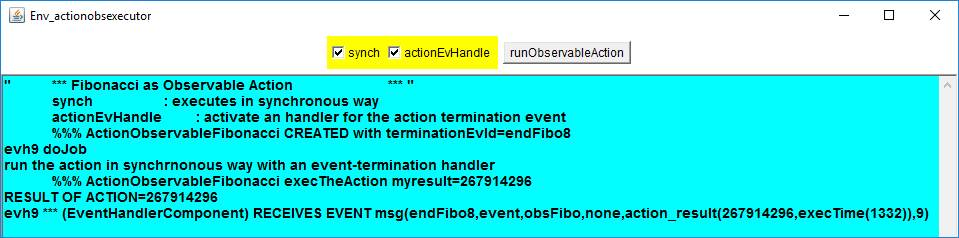
\includegraphics[scale = 0.6]{img/actionObs.jpg}\\
\end{tabular}{   }
\end{center}


 \newpage 
\subsection{Timed actions}
\labelssec{timedAction}

In several situations, an application designer could activate actions that must always terminate within a prefixed amount of time. In \xss{planactions} we have introduced the idea of \textit{timed action}.

We can define an \textit{\textbf{Timed Action}} as an \textit{Observable Action} whose execution time \texttt{T} satisfies the constraint \texttt{T<=DURATION}, where \texttt{DURATION} is a prefixed amount of time\footnote{Usually, \texttt{T} and \texttt{DURATION} are expressed in millisecs.}. Moreover:
\begin{itemize}
\item the action can be activated in two different ways: \textit{synchronous mode} and \textit{asynchronous mode};
\item a Timed Action activated in  \textit{\textbf{synchronous}} mode: \textit{i)} blocks the activator until the action is completed and \textit{ii)} emits a termination event when it ends its work;
\item a Timed Action activated in  \textit{\textbf{asynchronous}} mode:  \textit{i)} returns immediately the control to the activator, and \textit{ii)} emits a termination event when it ends its work;
\item a Timed Action can be \textit{\textbf{suspended}} (interrupted) even if it not already terminated. A Timed Action is called \textbf{\textit{recoverable}} if the action can resume its work after a suspension.
%%\item the \textit{\textbf{result}} of a Timed Action is an object (of type \texttt{AsynchActionResult}, see \xss{AsynchActionResult}) that the wraps the application result into a structure that gives other information about the action (e.g. interrupted or not, execution time remained with respect to the \texttt{DURATION}, etc.)
\end{itemize}

Thus, a Timed Action works in its own thread of control; its activator can decide to wait for the termination of the action (\textit{synchronous mode} activation) or to continue its work. In case of \textit{asynchronous mode} activation, an actor interested in the application result of the action can look at the \textit{termination event} emitted by the action. 

%%%If a timed action is suspended (since its duration expires) and it is recoverable, it can continue its execution later\footnote{An action can be also suspended for other reasons kind of behaviour is useful for example  when a robot must execute a move for some time, while being able to reacts to alarms.}. 

Timed Actions implement the following interface: 

\lstinputlisting[language=java,caption={ \texttt{IActorAction<T>} }, firstline=1 ]{../../../it.unibo.qactors/src/it/unibo/qactors/action/IActorAction.java}

\subsubsection{\texttt{ActorTimedAction}} class.\\
\labelssec{ActorAction} 
The class \texttt{ActorTimedAction} implements the concept of Timed Action by building a 'subsystem' composed of the action and other two components: a \textit{timer} and a \textit{event handler}:

%and is the basic building block for the different types of \textit{PlanActions} introduced in \xss{planactions}:

\medskip 
\begin{center}
\medskip 
\begin{tabular}{|c|c|}
\hline 
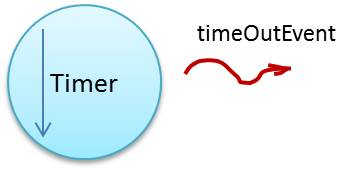
\includegraphics[scale = 0.7]{img/actionTimer.jpg} & 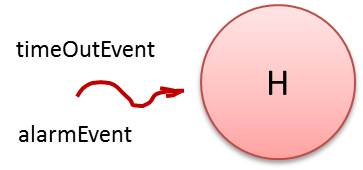
\includegraphics[scale = 0.5]{img/actionEventHandler.jpg} \\ 
\hline 
\end{tabular}
\end{center}

Let us report here the code related to action construction:

\lstinputlisting[language=java,caption={ \texttt{ActorTimedAction} }, firstline=1, lastline=50 ]{../../../it.unibo.qactors/src/it/unibo/qactors/action/ActorTimedAction.java}

The operation \textit{getActionBodyAsCallable} must be defined by the Application designer so to return a \texttt{Callable<T>} object that is run within a new Thread, in parallel with a Timer. The Timer is created in a specialized version of the operation \textit{startOfAction}, while the  \texttt{Callable<T>} is activated in a specialized version of the operation \textit{execTheAction}.

The architecture of the 'subsystem' built by the \texttt{initActorTimedAction} operation is shown in the following picture:

\begin{center}
\begin{tabular}{ c }
     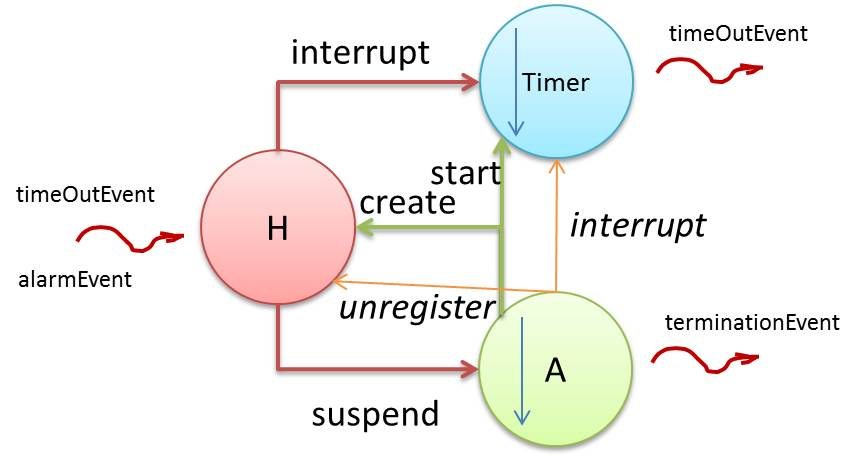
\includegraphics[scale = 0.7]{img/actionTimedReactive.jpg}\\
\end{tabular}{   }
\end{center}

The picture shows that the handler H can be activated  by a \texttt{timeOutEvent} or by an \texttt{alarmEvent}. The case of \texttt{alarmEvent} is related to the case of reactive actions, introduced in  \xss{reactiveactions}.

\subsubsection{Fibonacci as a Timed} Action.
\labelssec{fibotimed}

The \texttt{fibonacci} computation of \xss{basicactions} is defined in the following as a Timed Action that takes at construction time a goal of the form \texttt{fibo(N,V)} where \texttt{N} is the fibonacci number to evaluate and \texttt{V} is the (variable that denotes the) result.

\lstinputlisting[language=java,caption={ \texttt{ActionFibonacciTimed} }, firstline=1 ]{../../../it.unibo.qactors.tests/src/it/unibo/actiontimedexecutor/ActionFibonacciTimed.java}

\subsubsection{Experiments on Fibonacci as Timed} Action.\\

The project \textit{it.unibo.qactors.tests} includes the model \texttt{actionTimedDemo.qa} that shows the effects of the action in the different execution modes:

\lstinputlisting[language=qa,caption={ \texttt{actionTimedDemo.qa} }, firstline=1 ]{../../../it.unibo.qactors.tests/src/actionTimedDemo.qa }

  
 
\begin{center}
\begin{tabular}{ c }
     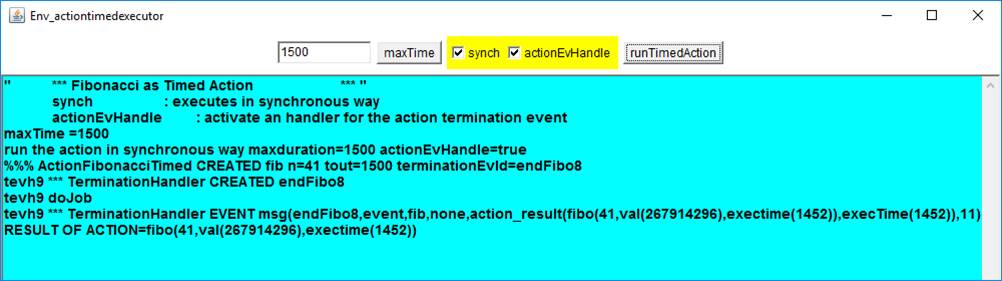
\includegraphics[scale = 0.6]{img/actionTimed.jpg}\\
\end{tabular} 
\end{center}



\newpage 
\subsection{Reactive actions}
\labelssec{reactiveactions}
We can define a \textit{\textbf{Reactive Action}} as a \textit{Timed Action} that can be suspended (interrupted) by the occurrence of events.  

The occurrence of an event E that suspends the execution of a reactive action RA in a plan P, gives raise to the execution of a plan EP associated to the event E. The plan EP, once terminated, can terminate the behaviour of the Actor or resume the plan P, that will be continue from the suspension point of the action RA, if it is recoverable, or from the action that follows RA in P.

%% The execution of a Reactive Action is done under the control of a \textit{TaskActionFsmExecutor} that is able to handle the action termination-event and any expected 'interruption' event (including a time-out) that can happen while the action is running. 

%%This Reactive Action executor is a specialization of an abstract \texttt{TaskComponent} that implements a event-based finite-state machine whose input-set is called \textit{inputSymbolEventsSet}. The run-time support resumes a Task only when the current event belongs to \textit{inputSymbolEventsSet} and this input is in the \textit{expectedInput} set of its current Task \textit{state}. This work is done by an event handler (of class \textit{TaskQueueEventHandler}) that:
%% \begin{itemize}
%% \item is automatically created when a new Task instance is created
%% \item reacts to all the events that belong to the  \textit{inputSymbolEventsSet} of the Task;
%% \item resumes the Task if it is not already activated;
%% \item stores the event in a local queue if the Task already activated.
%% \end{itemize}



\subsubsection{\texttt{AsynchActionResult}} class.\\
\labelssec{AsynchActionResult}
The \textit{\textbf{result}} of a Reactive Action is an object of type \texttt{AsynchActionResult} that  wraps the application result into a structure that gives other information about the action (e.g. interrupted or not, execution time remained with respect to the \texttt{DURATION}, etc.)

 
%% OLD pre akka \lstinputlisting[language=java,caption={ \texttt{AsynchActionGenericResult<T>} }, firstline=1  ]{../../../it.unibo.qactors/src/it/unibo/qactors/action/AsynchActionGenericResult.java}
\lstinputlisting[language=java,caption={ \texttt{AsynchActionResult<T>} }, firstline=1  ]{../../../it.unibo.qactors/src/it/unibo/qactors/action/AsynchActionResult.java}

It implements the following interface:
 
\lstinputlisting[language=java,caption={ \texttt{IAsynchActionResult.java} }, firstline=1 ]{../../../it.unibo.qactors/src/it/unibo/qactors/action/IAsynchActionResult.java}

\subsubsection{Fibonacci as a Reactive} Action.\\
\labelsec{fiboreactive}

 
The \texttt{fibonacci} computation of \xss{fibotimed} can be used to build a Reactive Action:
%%, by introducing a test to 'interrupt' the action if it has been suspended by some event.

\lstinputlisting[language=java,caption={ \texttt{ActionReactiveFibonacci<T>} }, firstline=1,lastline=25 ]{../../../it.unibo.qactors.tests/src/it/unibo/actionreactiveexecutor/ActionReactiveFibonacci.java}

\subsubsection{Experiments on Fibonacci as Reactive} Action.\\

 
The project \textit{it.unibo.qactors.tests} includes the model \texttt{actionReactiveDemo.qa} that shows the effects of the action in the different execution modes. When the \texttt{interrupt} flag is set, an event \texttt{usercnd : stop} is generated\footnote{The operation \texttt{e QActorUtils.emitEventAfterTime}  generates a given event after a given time.} after \texttt{maxtime/2} \textit{msecs}. 

\lstinputlisting[language=qa,caption={ \texttt{actionReactiveDemo.qa} }, firstline=1 ]{../../../it.unibo.qactors.tests/src/actionReactiveDemo.qa }

\begin{center}
\begin{tabular}{ c }
     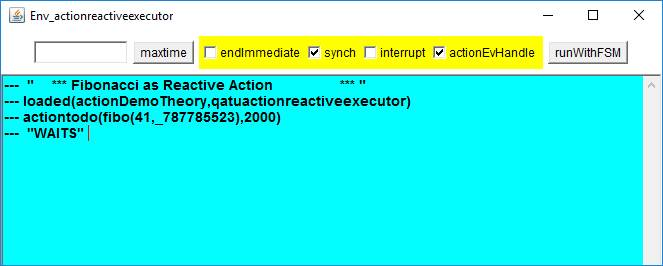
\includegraphics[scale = 0.6]{img/actionReactive.jpg}\\
\end{tabular} 
\end{center}




\newpage  
\section{An interpreter to execute actions}
\labelsec{aboutactions}

In this section we introduce a system that provides an interpreter allowing human users to execute actions expressed as commands sent via the interfaces introduced in \xs{humaninteraction}.
The model of the system is defined in the project \textit{it.unibo.qactors.tests}:

\lstinputlisting[language=qa,caption={ \texttt{cmdExecutor.qa} }, firstline=1 ]{../../../it.unibo.qactors.tests/src/cmdExecutor.qa}

The interpreter is written in Prolog in the user theory stored in file \texttt{talkTheory.pl}.

It works with reference to a simple syntax that we will introduce in the examples that follows. Since the syntax is at the moment quite limited, only a subset of actions can be executed.  For example, since the symbol \texttt{':-'} ' is not admitted, we cannot execute actions like \texttt{ addRule(r(X):-q(X))}.

\subsection{Basic actions}
\labelssec{basicactions}


Basic actions can be expresses as follows:
\begin{Verbatim} [fontsize=\scriptsize, frame=single, label=Timed Action syntax structure]
ACTION 
\end{Verbatim}

A basic action is a terminating action that implements an algorithm written in Java, tuProlog or in some other executable language (for example C or C++). 
For example:

\begin{Verbatim} [fontsize=\scriptsize, frame=single, label=Basic actions]
fib(7,V)
raise(alarm,alarm(fire))
play('./audio/tada2.wav')
\end{Verbatim}


\subsection{Guarded actions}
\labelssec{guardedaction}

Actions prefixed by a guard can be expressed as follows:
\begin{Verbatim} [fontsize=\scriptsize, frame=single, label=Guarded Action syntax structure]
[ GUARD ] , ACTION , ... 
\end{Verbatim}

They are executed only if the \texttt{GUARD} is evaluated \texttt{true}. The \texttt{GUARD} is a boolean condition expressed as a \prolog{} term that can include unbound variables, possibly bound during the guard evaluation phase.
%
%%% For example, the following action plays a sound for a time \texttt{T} given by the evaluation of the guard \texttt{execTime/1}:
%%% \begin{Verbatim} [fontsize=\scriptsize, frame=single, label=A guarded action]		
%%% [ execTime(T) ] , play('./music_interlude20.wav') , T  
%%% \end{Verbatim}

For example, the following action plays a sound only if the evaluation of the guard \texttt{goon/0} ends with success\footnote{No variables are supported in this version of the interpreter.}:
\begin{Verbatim} [fontsize=\scriptsize, frame=single, label=guards]	
[  goon ], play('./audio/music_interlude20.wav'),20000,'alarm,obstacle', 'handleAlarm,handleObstacle'
\end{Verbatim}

The evaluation of the guard will end with success, if we send the command:
\begin{Verbatim} [fontsize=\scriptsize, frame=single, label=guards]	
addRule( goon )
\end{Verbatim}

\subsection{Timed actions}
\labelssec{timedaction}
Time actions can be expresses as follows:
\begin{Verbatim} [fontsize=\scriptsize, frame=single, label=Timed Action syntax structure]
[ GUARD ] , ACTION , DURATION 
\end{Verbatim}
For example, the action:
\begin{Verbatim} [fontsize=\scriptsize, frame=single, label=Timed actions]		
play('./audio/tada2.wav') , 1000  
\end{Verbatim}
must terminate within a time \texttt{T<=1000 msec}.
During the time \texttt{T} the actor does not execute any other new action; thus, it cannot accept other commands.  

\subsection{Time out}
\labelssec{timeout}
If a time-out expires, the fact
\begin{Verbatim} [fontsize=\scriptsize, frame=single, label=Timed actions]
tout(EVENTID,QACTORID). 
\end{Verbatim} 

\noindent is asserted in the \textit{WorldTheory} of the working \qa. This fact can be used to execute actions under the control of a guard (see \xss{guardedaction} ); for example:

\begin{Verbatim} [fontsize=\scriptsize, frame=single, label=Timed actions]
[ tout(E,A) ] , switchToPlan handleTout
\end{Verbatim}

\subsection{Asynchronous actions}
\labelssec{asynchaction}
Actions of the form:
\begin{Verbatim} [fontsize=\scriptsize, frame=single, label=Asynchronous Action syntax structure]
[ GUARD ] , ACTION , DURATION , ENDVENT 
\end{Verbatim}

that specify  a \textit{\textbf{non-empty}} \texttt{ENDEVENT} atom, are activated in asynchronous way. Each asynchronous action works in a proper \textit{Thread} and emits the specified \texttt{ENDEVENT} at termination.
For example:
 
\begin{Verbatim} [fontsize=\scriptsize, frame=single, label=Asynchronous action]		
play('./audio/tada2.wav') , 1500  , endplay
\end{Verbatim}

\noindent is a timed, asynchronous \texttt{play} action that returns immediately the control. Thus the robot is able to perform other actions 'in parallel' with the previous one. When the \texttt{play} action terminates (after \texttt{1500} msecs), the event named \texttt{endplay} is raised.

Asynchronous actions cannot be reactive (see \xss{reactiveaction}). This because the idea of reacting to an asynchronous actions must be further explored.

\subsection{Reactive actions}
\labelssec{reactiveaction}
Actions of the form:
\begin{Verbatim} [fontsize=\scriptsize, frame=single, label=Reactive Action syntax structure]
[ GUARD ] , ACTION , DURATION , [EVENTLIST], [PLANLIST]
\end{Verbatim}

that specify  a \textit{\textbf{non-empty}} \texttt{EVENTLIST} and \texttt{PLANLIST} are called synchronous \textbf{\textit{reactive actions}} since they can be 'interrupted' by one of the events specified in the \texttt{EVENTLIST}. When one of these events occurs, the action is 'interrupted' and the corresponding plan specified in the \texttt{PLANLIST} is put in execution.

For example, the action:
\begin{Verbatim} [fontsize=\scriptsize, frame=single, label=Reactive Action]
play('./audio/music_interlude20.wav') , 20000 , [usercmd,alarm], [handleUsercmd,handleAlarm]
\end{Verbatim}
is an example of a play action that must terminate within \texttt{20 secs}. During this time, the occurrence of an event named \texttt{usercmd} or \texttt{alarm} terminates the action and puts in execution the plan \texttt{handleUsercmd} or \texttt{handleAlarm} respectively.

Reactive actions cannot be activated in asynchronous way, since the idea of reacting to an asynchronous actions must be further explored. 


	
%% A reactive action is implemented as a \textit{finite state}, event-based (see \xs{events} ) machine.

\newpage  
	\section{Interactions using \texttt{MQTT} (to be completed)}
\labelsec{usemqtt}
 
The \texttt{MQ} \textit{Telemetry Transport} (\texttt{MQTT}) is an ISO standard (ISO/IEC PRF 20922) publish-subscribe based "light weight" messaging protocol for use on top of the TCP/IP protocol. It is useful for connections with remote locations where a small code footprint is required and/or network bandwidth is at a premium.

The \textit{Eclipse Paho} project provides open-source client implementations of \texttt{MQTT} and \texttt{MQTT-SN} (\textit{MQTT For Sensor Networks}\footnote{\texttt{MQTT-SN} is a protocol derived from \texttt{MQTT}, designed for connectionless underlying network transports such as \texttt{UDP}}) messaging protocols aimed at new, existing, and emerging applications for \textit{Machine-to-Machine} (\texttt{M2M}) and \textit{Internet of Things} (\texttt{IoT}). There are already \texttt{MQTT} \texttt{C} and \java{} libraries with \texttt{Lua}, \texttt{Python}, \texttt{C++} and \texttt{JavaScript} at various stages of development.


The usage of the \texttt{MQTT} protocol can be delegated to rules defined by the application designer in some theory, e.g. a \texttt{mqttTheory.pl}. 

\subsection{The mqttTheory}
The \texttt{mqttTheory} that 'extends' the \texttt{qa} action-set with new operations for the usage of the \texttt{MQTT} protocol can be defined as follows:

\lstinputlisting[language=pl,caption={ The \texttt{mqttTheory.pl} }, firstline=1 ]{../../../it.unibo.ddr.avatar/mqttTheory.pl}


These rules in their turn make use of a \java{} utility object of class \texttt{MqttUtils}.

\subsection{The MqttUtils}
The \java{} utility class to be used as a support for \texttt{MQTT} interaction can be defined as follows:

\lstinputlisting[language=java,caption={ The utility class \texttt{MqttUtils.java} }, firstline=1 ]{../../../it.unibo.ddr.avatar/src/it/unibo/mqtt/utils/MqttUtils.java}

An object of class \texttt{MqttUtils} is used as a \textit{singleton} and works as the support for the actor that calls the operation \texttt{connect} (that creates a \texttt{MqttClient}).

The \texttt{subscribe} operation sets this singleton support as the object that provides the callback (\texttt{messageArrived}) to be called when the \texttt{MqttClient} is a subscriber. The callback is defined so to map a \texttt{MqttMessage} into a dispatch of the form:

\begin{Verbatim}[fontsize=\scriptsize, frame=single]
mqttmsg : mqttmsg( TOPIC,PAYLOAD )
\end{Verbatim}

This dispatch is then sent to the actor that uses the singleton support, i.e. that works as a \texttt{MqttClient} (subscriber).


 
 
\newpage
\section{Introduction to QRobots}
\labelsec{introQRobots}
 
Since a \texttt{QRobot} (see \xs{QRobot} ) is a \texttt{QActor} able to interact with an instance of a \textit{BaseRobot}, we must first of all understand what is a \textit{BaseRobot}.
%%, as shown in the following picture:

%% \begin{center}
%%\begin{tabular}{ c }
%%     \includegraphics[scale = 0.65]{../../../it.unibo.iss2015intro/docs/Robots/robotActor.jpg}\\
%%\end{tabular} 
%%\end{center}

\medskip 
From the physical point of view, a \texttt{BaseRobot} is a custom device built with low-costs components including sensors, actuators and processing units like \textit{RaspberryPi} and \textit{Arduino}. Examples are given in the following picture:

\begin{center}
\begin{tabular}{ c }
     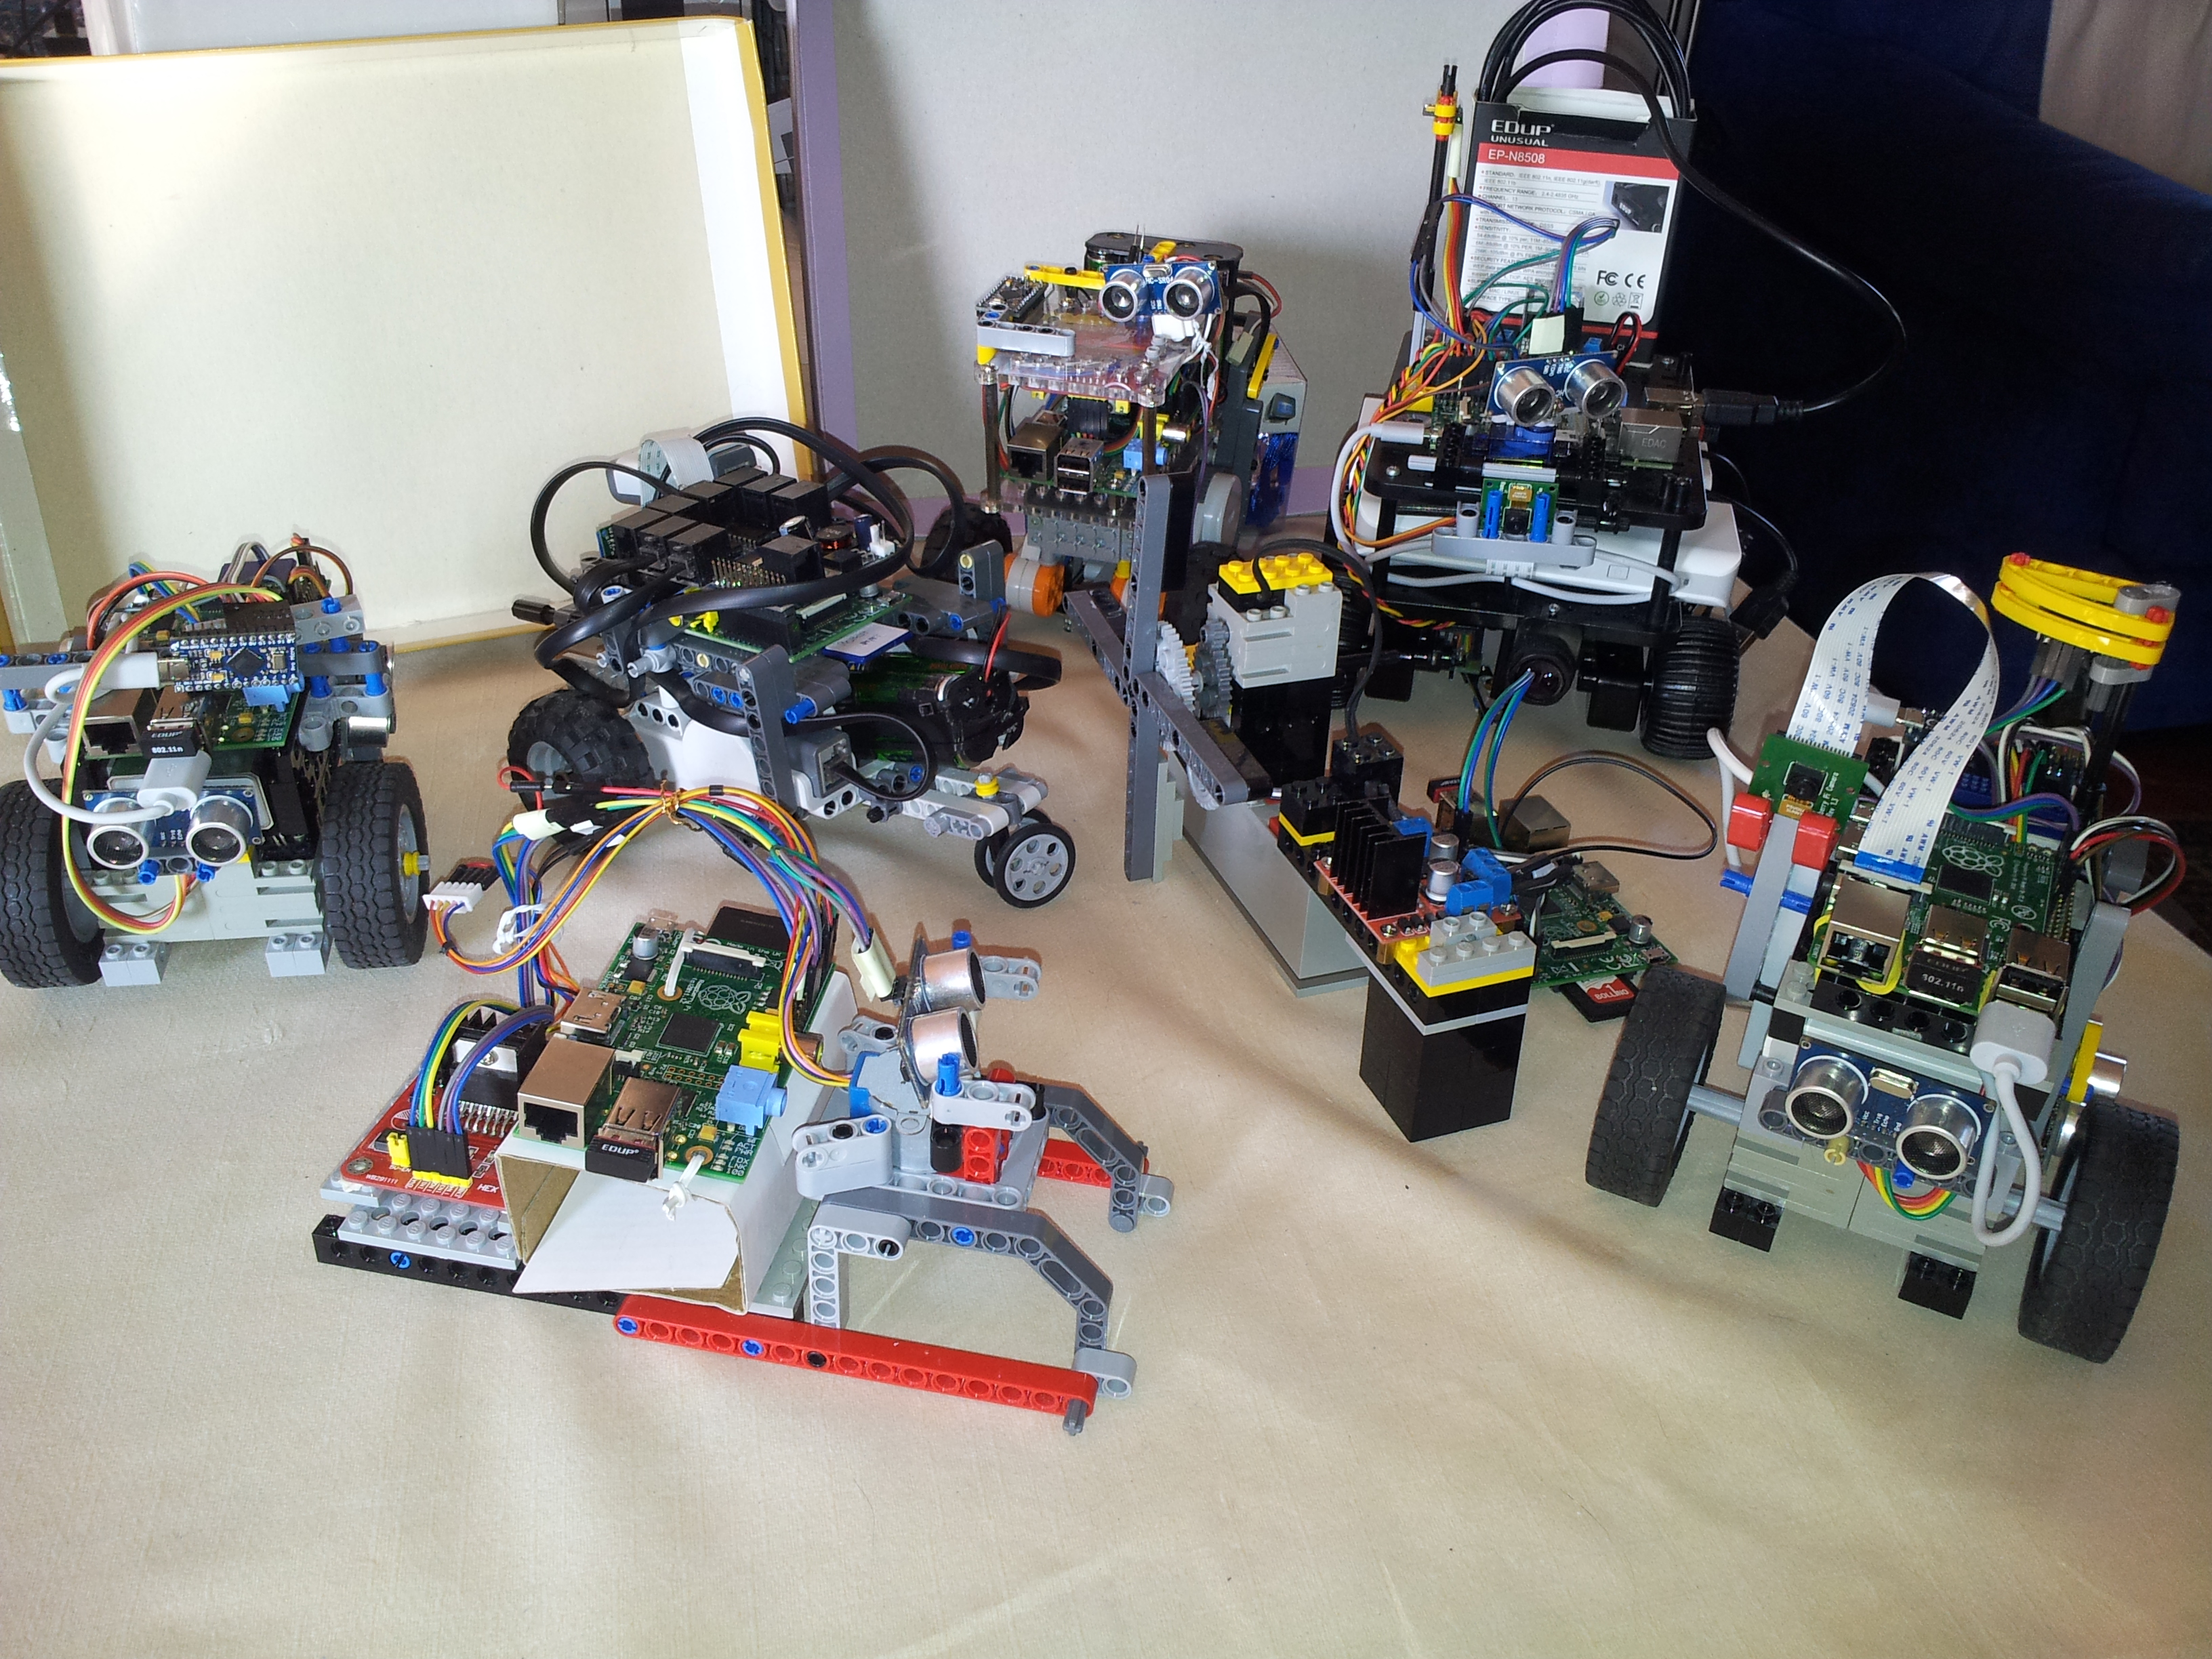
\includegraphics[scale = 0.09]{../../../it.unibo.iss2015intro/docs/imgs/robot/customDevs.jpg}\\
\end{tabular} 
\end{center}


The hardware components of a \texttt{BaseRobot} and their configuration can be quite different from robot to robot. Thus, some software layer is required to hide these differences as much as possible and to build a 'technology independent' layer, to be used by application designers.

A software layer of this kind is provided by the library \textit{labbaseRobotSam.jar}. More specifically:  


\medskip 
\noindent 
\begin{tabular}{|p{0.30\textwidth}|p{0.70\textwidth}|}
\hline 
\textit{it.unibo.lab.baseRobot } 
&The basic software for differential drive robots that are able to move and to acquire sensor data. 

\medskip 
Library: \textit{labbaseRobotSam.jar}. 
\\ 
\hline 
\textit{it.unibo.lab.baseRobot.example} 
&Example of the usage of the \texttt{API} of a BaseRobot.
\\ 
\hline 
\end{tabular} 


\section{A model for the BaseRobot}
\labelssec{BaseRobotModel}

The main goal of the \textit{labbaseRobotSam.jar} library is to simplify the work of an application designer by exposing at application level a very simple model of a \texttt{BaseRobot}:

\begin{itemize}
\item As regards the \textbf{\textit{structure}}, a \texttt{BaseRobot} can be viewed as a entity composed of two main parts:
\begin{itemize}
\item An executor (with interface \texttt{IBaseRobot}), able to move the robot according to a  a prefixed set of movement commands (\texttt{IBaseRobotCommand}) 
\item A set of GOF-observable sensors (each with interface \texttt{ISensor}), each working as an active source of data.
\end{itemize}
\item As regards the \textbf{\textit{interaction}}, a \texttt{BaseRobot} can be viewed as a POJO that implements the interface \texttt{IBaseRobot}, while providing a (possibly empty) set of observable sensors;
\item  As regards the \textbf{\textit{behavior}}, a \texttt{BaseRobot} is an object able to execute \texttt{IBaseRobotCommand} and able to update sensor observers defined by the application designer.
\end{itemize}


\begin{center}
\begin{tabular}{ c }
     \includegraphics[scale = 0.8]{../../../it.unibo.lab.baseRobot/umlModels/BasicRobot.jpg}\\
\end{tabular} 
\end{center}

The interface \texttt{IBasicRobot} is introduced as a (GOF) \textit{Facade} for the model.
\lstinputlisting[language=java,caption={ \texttt{IBasicRobot.java} }, firstline=1  ]{../../../it.unibo.lab.baseRobot/src/it/unibo/iot/baseRobot/hlmodel/IBasicRobot.java}

\subsection{The BasicRobot class}
\labelssec{BasicRobot}

The class \texttt{BasicRobot} provides a factory method to create a \texttt{BaseRobot} and to select its main components.

\lstinputlisting[language=java,caption={ \texttt{BasicRobot.java} }, firstline=1  ]{../../../it.unibo.lab.baseRobot/src/it/unibo/iot/baseRobot/hlmodel/BasicRobot.java}

This class shows that the work to set-up and access to the internal structure of a \texttt{BaseRobot} is delegated to a  \texttt{Configurator}. This Configurator reads the specification of the robot structure written in a file named \textit{iotRobot.properties}.   



\subsection{Using a BaseRobot}
\labelssec{}

Let us introduce (project \textit{it.unibo.lab.baseRobot.example}) a robot with configuration named \texttt{\textbf{mocksimple}}, equipped with two motors and a distance sensor, all simulated. 

\subsubsection{The project workspace}
\labelssec{workspace}

The application designer must organize its project workspace as shown in the following snapshot:

\begin{center}
\begin{tabular}{ c }
     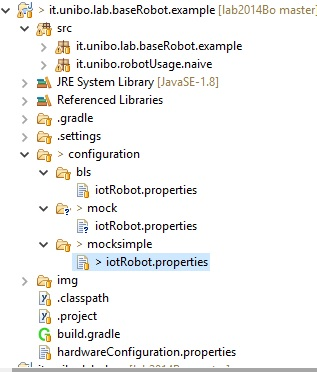
\includegraphics[scale = 0.7]{./img/baseRobotProject.jpg}\\
\end{tabular} 
\end{center}

\subsubsection{The code}
\labelssec{workspace}

The application: \textit{i)} first creates a sensor observer and adds it to all the sensors; \textit{ii)} then it tells the robot to execute the commands it is able to understand.

\lstinputlisting[language=java,caption={ \texttt{BasicRobotUsageNaive.java} }, firstline=1  ]{../../../it.unibo.lab.baseRobot.example/src/it/unibo/robotUsage/naive/BasicRobotUsageNaive.java}

\begin{center}
\begin{tabular}{ c }
     \includegraphics[scale = 0.7]{../../../it.unibo.lab.baseRobot/umlModels/CommandModel.jpg}\\
\end{tabular} 
\end{center}

\subsection{The work of the Configurator}
\labelssec{Configurator}

An object of class \textit{it.unibo.iot.configurator.Configurator}:
\begin{enumerate}
\item first looks at the file \texttt{hardwareConfiguration.properties} to get the name of the robot (e.g. mock)
\item then, it consults the file \texttt{iotRobot.properties} into the directory \texttt{configuration/mock}
\end{enumerate}
 
For each specification line, the \texttt{Configurator} calls (by using Java reflection) a factory method of the specific \texttt{DeviceConfigurator} class associated to the name of the robot.

For example, let us consider a Mock robot equipped with two motors and a distance sensor, all simulated:
(file \textit{configuration/mocksimple/iotRobot.properties}):
\lstinputlisting[language=qa,caption={ \texttt{configuration/mocksimple/iotRobot.properties} }, firstline=1  ]{../../../it.unibo.lab.baseRobot.example/configuration/mocksimple/iotRobot.properties}

The Configurator calls (using an object of class \texttt{IotComponentsFromConfiguration}):
\begin{itemize}
\item \texttt{getMotorDevice} of \textit{it.unibo.iot.device.mock.DeviceConfigurator} \\ (for \textbf{motor.left=mock})
\item \texttt{getBaseRobotDevice} of \textit{it.unibo.iot.device.differentialdrive.DeviceConfigurator} \\(for \textbf{baserobot.bottom=differentialdrive})
\item \texttt{getDistanceSensorDevice} of \textit{it.unibo.iot.device.mock.DeviceConfigurator} \\(for \textbf{distance.front=mock})
\item \texttt{getMotorDevice} of \textit{it.unibo.iot.device.mock.DeviceConfigurator} \\(for \textbf{motor.right=mock})
\item \texttt{getActuatorsDevice} of \textit{it.unibo.iot.device.ddmotorbased.DeviceConfigurator} \\(for \textbf{actuators.bottom=ddmotorbased})
\end{itemize}


\subsection{From mocks to real robots}
\labelssec{}

In order to use a physical robot rather than a Mock robot, the software designer must simply change the specification of the robot configuration; the application code is unaffected. For example, to use our standard '\texttt{nano}' robots, we have to include into the \texttt{configuration/nano} directory the following configuration file:

\lstinputlisting[language=qa,caption={ \texttt{configuration/nano/iotRobot.properties  } }, firstline=1  ]{../../../it.unibo.lab.baseRobot.example/configuration/nano/iotRobot.properties}

\newpage 
\section{Sensors and Sensor Data}
\labelsec{Sensors}
 
The current version of the \texttt{BaseRobot} system implements the following sensors:
\begin{verbatim}
 RobotSensorType: Line | Distance | Impact | Color | Magnetometer  
\end{verbatim} 

Each sensor:
\begin{itemize}
\item is associated to a position that can assume one of the following values:
\begin{verbatim}
	DONTCARE| 
	FRONT | RIGHT | LEFT | BACK | TOP | BOTTOM |
	FRONT_RIGHT | FRONT_LEFT | BACK_RIGHT | BACK_LEFT | 
	TOP_RIGHT | TOP_LEFT | BOTTOM_RIGHT | BOTTOM_LEFT |
	FRONT_TOP | BACK_TOP | FRONT_TOP_LEFT | FRONT_TOP_RIGHT |
	FRONT_RIGHT_TOP | FRONT_LEFT_TOP | BACK_RIGHT_TOP | BACK_LEFT_TOP 
\end{verbatim}
\item is a source of data, each associated to a specific class and interface:     
\begin{center}
\begin{tabular}{ c }
     \includegraphics[scale = 0.45]{../../../it.unibo.lab.baseRobot/umlModels/SensorData.jpg}\\
\end{tabular} 
\end{center}
\end{itemize}

Each class related to sensor data inherits from a base class \texttt{SensorData}. For example:

\begin{center}
\begin{tabular}{ c }
     \includegraphics[scale = 0.4]{../../../it.unibo.lab.baseRobot/umlModels/SensorDataClasses.jpg}\\
\end{tabular} 
\end{center}


The class \texttt{SensorData} provides operations to represent data as strings in two main formats: \textit{i)} in \texttt{Prolog} syntax and \textit{ii)} in \texttt{Json} syntax. For example:

\subsubsection{Sensor data representation in Prolog (high level)}
%% {\footnotesize
\begin{flushleft}
\begin{tabular}{|l|l|l|}
\hline 
COLOR & color(255 255 255, front)  \\ 
\hline 
DISTANCE & distance(43,forward, front)   \\ 
\hline 
IMPACT  & impact(touch/loss, front)   \\ 
\hline 
LINE & line(lineLeft/lineDetected, bottom)   \\ 
\hline 
MAGNETOMETER & magnetometer(x(50),y(100),z(0), front)   \\ 
\hline 
\end{tabular} 
\end{flushleft}
%% }

\subsubsection{Sensor data representation in Json (low level)}
  
\begin{flushleft}
\begin{tabular}{|l|l|l|}
\hline 
COLOR &  {"p":"f","t":"c","d":{"color":{"r":255,"b":255,"g":255}},"tm":148...} \\ 
\hline 
DISTANCE  & {"p":"f","t":"d","d":{"cm":43},"tm":14...} \\ 
\hline 
IMPACT   & {"p":"f","t":"i","d":{"detection":"touch"},"tm":14...} \\ 
\hline 
LINE  & {"p":"b","t":"l","d":{"detection":"lineDetected"},"tm":14...} \\ 
\hline 
MAGNETOMETER  & {"p":"f","t":"m","d":{"raw3axes":{"x":50,"y":100,"z":0}},"tm":14...} \\ 
\hline 
\end{tabular} 
\end{flushleft}
 

\subsection{Sensor model}
\labelssec{Sensormodel}
The sensor subsystem of the \texttt{BaseRobot} is based on the class \texttt{Sensor} that represents a sensor from the logical point of view. Each sensor is associated to a class that inherits form \texttt{Sensor}.

\begin{center}
\begin{tabular}{ c }
     \includegraphics[scale = 0.4]{../../../it.unibo.lab.baseRobot/umlModels/ButtonAsSensor.jpg}\\
\end{tabular} 
\end{center}

The model reported in the picture above shows that:
\begin{itemize}
	\item A \texttt{DistanceSensor} is a logical \texttt{Sensor} associated (by the \textit{Configurator}) to a concrete device (e.g. \texttt{DistanceHcsr04SensorDevice}). The same is true for a \texttt{ButtonSensor} (impact).
	\item A \texttt{DistanceHcsr04SensorDevice} is a concrete \texttt{SensorDevice} that updates its logical sensor when it produces a value. The same is true for a \texttt{DistanceButton} (impact). The diagrma shows also a \texttt{MockDevice} that can be used to simulate the behavior of the supported sensors.
	\item Any \texttt{Sensor} is an observable entity that, when updated from its concrete device, updates the registered application observers.
\end{itemize}

In this way, according to the GOF pattern \textit{Bridge}, the \texttt{Sensor} abstraction hierarchy is decoupled from the hierarchy of \texttt{SensorDevice} implementation.



A more detailed picture is reported hereunder:
 
\begin{center}
\begin{tabular}{ c }
     \includegraphics[scale = 0.4]{../../../it.unibo.lab.baseRobot/umlModels/RobotsSensorModel.jpg}\\
\end{tabular} 
\end{center}



\section{Actuators and Executors}
\labelsec{Actuators}
 
The GOF Bridge pattern has been adopted also to model the 'motors' and the more general concept of 'executor'.

\begin{center}
\begin{tabular}{ c }
     \includegraphics[scale = 0.45]{../../../it.unibo.lab.baseRobot/umlModels/BaseRobotExecutor.jpg}\\
\end{tabular} 
\end{center}

However this part of the \texttt{BaseRobot} can be ignored by the application designer and it is no more discussed here.


\newpage 
\section{The QRobot }
\labelsec{QRobot}
Modelling a robot like a \texttt{POJO} is not adequate in those application problems in which a robot should be viewed as a proactive entity, able to interact (via message-passing) with other robots or with some control unit and to react to events related to the external world (e.g. an alarm an obstacle) or to its internal behavior (e.g. low battey level).

To deal with this kind of problems, the concept of \texttt{QActor} is introduced, with the goal to endow a \textit{BaseRobot} with new capabilities as regards the interaction.

From a conceptual point of view, a \texttt{QRobot} is a \texttt{QActor} that makes use of an instance of a \textit{BaseRobot}.
From a practical point of view, a \texttt{QRobot} is an instance of a class \texttt{RobotActor} (defined in the project \textit{it.unibo.qactor.robot}) that inherits form \texttt{QActor}. The class \texttt{RobotActor} provides the run time support for the differential drive model, whose structure, interaction and behavior can be expressed in a custom \texttt{DSL} named \texttt{ddr}.

 
\begin{center}
\begin{tabular}{ c }
    %% \includegraphics[scale = 0.6]{../../../it.unibo.iss2015intro/docs/Robots/robotActor.jpg}\\
    \includegraphics[scale = 0.6]{../../../it.unibo.lab.baseRobot/umlModels/RobotActor.jpg}\\
\end{tabular} 
\end{center}


\medskip 
The set of projects related to the idea of \texttt{QRobot} is reported in the following table:

\noindent
%% \begin{scriptsize}
\begin{tabular}{|p{0.28\textwidth}|p{0.72\textwidth}|}
\hline 
\textit{it.unibo.xtext.robot.base} 
&The metamodel (file extension \texttt{.baseddr})  for ddr-robot configuration.

\medskip 
Plugin: \textit{it.unibo.xtext.robot.base\_1.0.0.jar} 

Plugin: \textit{it.unibo.xtext.robot.base.ui\_1.0.0.jar}
\\ 
\hline 
\textit{it.unibo.xtext.qactor.robot} 
&The metamodel (file extension \texttt{.ddr}) that extends the \texttt{QActor} metamodel with concepts related to a \texttt{ddr}.

\medskip 
Plugin: \textit{it.unibo.xtext.qactor.robot\_1.3.4.jar}

Plugin: \textit{it.unibo.xtext.qactor.robot.ui\_1.3.4.jar}.
\\ 
\hline 
\textit{it.unibo.qactor.robot} 
&The run time support for \texttt{ddr} robots as qactors.

\medskip 
Library: \textit{uniboQactorRobot.jar}
\\
\hline 
\textit{it.unibo.xtext.qactor} 
&The metamodel (file extension \texttt{.qa}) that defines the \texttt{QActor} metamodel .

\medskip 
Plugin: \textit{it.unibo.xtext.qactor\_1.3.4.jar}

Plugin: \textit{it.unibo.xtext.qactor.ui\_1.3.4.jar}.
\\ 
\hline 
\textit{it.unibo.qactors} 
&The run time support for  qactors.

\medskip 
Library: \textit{qa18Akka.jar}
\\
\hline 
\textit{it.unibo.qactor.robot.avatar} 
&Examples of the usage of the \texttt{ddr} language/metamodel.
\\ 
\hline 
\end{tabular} 
 
\medskip 
The application designer can specify the logical structure, interaction and behavior of a \texttt{QRobot} by using a custom meta-model language (the \texttt{ddr} language), defined as an extension of the \texttt{qa} language introduced in \xs{introqa}.

\subsection{Command a QRobot from a console }

A \texttt{QRobot} is defined as a \texttt{QActor} able to perform physical moves and to perceive sensor data from the physical environment. Thus the user should be able to ask the robot to execute basic move actions in a 'naive' way or as timed or reactive actions.

\medskip 
\noindent
\begin{footnotesize}
\begin{tabular}{|p{0.5\textwidth}|p{0.5\textwidth}|}
\hline 
\texttt{ move(mf,100,0) } & move forward with full speed   \\ 
\hline 
\texttt{ move(mf,100,0),1000 } & move forward with full speed for 1 sec  \\ 
\hline 
\texttt{ move(mf,100,0),3000,endmove } & move forward with full speed for 3 secs in asynchronous way and at the end emits the event \texttt{endmove} \\
\hline 
\texttt{ move(mf,100,0),3000,[alarm],[handleAlarm] } & move forward with full speed for 10 sec and reacts to the 'alarm' event \\ 
\hline 
\end{tabular} 
\end{footnotesize}

\subsection{An Avatar}
\labelssec{avatar}

The project \textit{it.unibo.qactor.robot.avatar}  gives an example of a ddr-robot working as a device that executes commands sent from a user console (embedded in a browser):

\lstinputlisting[language=ddr,caption={ \texttt{avatar.ddr} }, firstline=1  ]{../../../it.unibo.qactor.robot.avatar/src/avatar.ddr}

\subsection{High Level Description of robot configuration }

Besides this specification, the application designer should also define (with the help of a system designer, if it is necessary) a high level robot configuration file. For example:

\lstinputlisting[language=ddr,caption={ \texttt{uniboMock.baseddr} }, firstline=1  ]{../../../it.unibo.qactor.robot.avatar/src/uniboMock.baseddr}


\lstinputlisting[language=ddr,caption={ \texttt{uniboNano.baseddr} }, firstline=1  ]{../../../it.unibo.qactor.robot.avatar/src/uniboNano.baseddr}

In particular:

\begin{itemize}
\item In the \textit{mocksimple} robot, all the actuators (motors) and the sensors are simulated.
\item In the \textit{nano0} robot, the motors and a sonar are directly connected to a RaspberryPi, while - in the commented lines - another sonar, a magnetometer and a lime detector are  connected, via serial line, to another device (e.g. an Arduino-Micro).
\end{itemize}

From the \texttt{avatar.ddr} specification, the \texttt{QRobot} software factory (project \textit{it.unibo.xtext.robot.base}) generates:
\begin{itemize}
\item A file \texttt{configuration/mocksimple/iotRobot.properties} 
\lstinputlisting[language=ddr,caption={ \texttt{configuration/mocksimple/iotRobot.properties} }, firstline=1  ]{../../../it.unibo.qactor.robot.avatar/configuration/mocksimple/iotRobot.properties}

\item A file \texttt{configuration/nano0/iotRobot.properties} 
\lstinputlisting[language=ddr,caption={ \texttt{configuration/nano0/iotRobot.properties} }, firstline=1  ]{../../../it.unibo.qactor.robot.avatar/configuration/nano0/iotRobot.properties}

\end{itemize}

 
\subsection{Sensors}
\labelssec{sensors}

Sensors are implemented as observable \texttt{POJO} (see \xss{sensorModel}). The generated class \texttt{SensorObserver} delegates to the rule \texttt{sensor/1} of \textit{sensorTheory} (see \xss{sensorTh}) the policy to handle the sensor data.

\lstinputlisting[language=java,caption={ \texttt{SensorObserver.java} }, firstline=1  ]{../../../it.unibo.qactor.robot.avatar/src/it/unibo/avatar/SensorObserver.java}

%%% \subsubsection{The sensor Theory.}
%%% \labelssec{sensorTh}

%%% The \textit{sensorTheory} is generated (only once) in the \texttt{src} directory in order to allow the application designer to introduce sensor handling rules related to the application logic. Its initial content is defined as follows:
%%% 
%%% \lstinputlisting[language=ddr,caption={ \texttt{sensorTheory.pl }, firstline=1  ]{../../../it.unibo.qactor.robot.avatar/sensorTheory.pl}

\subsubsection{Sensors handled by Arduino.}

The file \texttt{uniboArduinoBaseSupport.ino} in project \textit{it.unibo.qactor.robot} provides a support to handle motors and sensors coherent with  the assumptions of \textit{it.unibo.lab.baseRobot}:
 
\lstinputlisting[language=ddr,caption={ \texttt{uniboArduinoBaseSupport.ino} }, firstline=1 , lastline = 48 ]{../../../it.unibo.qactor.robot/arduino/uniboArduinoBaseSupport/uniboArduinoBaseSupport.ino}

\subsection{A model of serial.}

\begin{center}
\begin{tabular}{ c }
     \includegraphics[scale = 0.35]{../../../it.unibo.iss2015intro/docs/Robots/RobotSerialModel.jpg}\\
\end{tabular} 
\end{center}

\newpage   
\section{Motors (to be completed)}
\labelssec{motors}

Let us report here an example of using the \texttt{GPIO} library to control a motor via \texttt{PWM}

\lstinputlisting[language=java,caption={ \texttt{nanoMotorDriveA.sh} }, firstline=1  ]{../../../it.unibo.qactor.robot/lowLevel/nanoMotorDriveA.sh
}

\subsubsection{Servo}
\labelssec{servo}

\subsubsection{The pi-blaster.}
\labelssec{piblaster}
The pi-blaster project enables \texttt{PWM} on the \texttt{GPIO} pins. If we start pi-blaster without any parameters, it will enable \texttt{PWM} on the default pins;
\begin{verbatim}
cd /home/pi/pwm/piBlaster/
sudo ./pi-blaster
Channel number    GPIO number   Pin in P1 header
      0               4             P1-7
      1              17             P1-11
      2              18             P1-12
      3              21             P1-13
      4              22             P1-15
      5              23             P1-16
      6              24             P1-18
      7              25             P1-22
Set GPIO pin 17 to a PWM of 20%
echo "17=0.2" > /dev/pi-blaster
\end{verbatim}      

 
%%\section{Interacting with physical robots}
%%\labelsec{physrobot} 


\subsubsection{Xtext installation}
\labelssec{}


\begin{enumerate}
\item download and install 64-bit JRE and add the path to it in eclipse.ini. For example:
\begin{verbatim}
...
--launcher.appendVmargs
-vm
C:\Program Files\Java\jre1.8.0_45\bin\javaw.exe
-vmargs
...
\end{verbatim}
The -vm parameter should be just before -vmargs and the path should be on a separate line. It should be the full path to the javaw.exe file. Do not enclose the path in double quotes (").

\item  download eclipse neon for Java developers
\item  install xtext plugins from (install new software site)
\begin{verbatim}
http://download.eclipse.org/modeling/tmf/xtext/updates/composite/releases/
\end{verbatim}
\item  download ecore diagram plugin
\begin{verbatim}
http://download.eclipse.org/ecoretools/updates/releases/3.2.0/neon
\end{verbatim}
\item check for updates
\item Window -> Preferences -> General -> Startup and Shutdown and uncheck "RSE UI".
\item Remove slf4j-simple from your dependencies, logback-classic is enough.
\end{enumerate}

 



 

 

 
 
%%  \section{About actions}
\labelsec{aboutactions}

In \xss{actions} we said that an \textit{\textbf{action}} is an activity that must always terminate. The effects of an action can be perceived as changes in the logical or in the physical actor environment.

Let us consider here an action that computes the \texttt{n-th} number of Fibonacci (slow, recursive version):

\begin{javacode}
	protected long fibonacci( int n ){
		if( n<0 || n==0 || n == 1 ) return 1;
		else return fibonacci(n-1) + fibonacci(n-2);
	}
\end{javacode}

Usually an action expressed in this way is executed as a procedure that keeps the control until the action is terminated. Since this a 'pure computational action', its effects can be perceived (as a result of type \texttt{long}) when the action returns the control to the caller.


\subsection{Asynchronous Observable Actions}
\labelssec{actionObservable}

Let us introduce now a new idea of an action\footnote{The growing demand for asynchronous, event-driven, parallel and scalable systems demand for new abstractions.} , with the following properties:
\begin{enumerate}
\item the action performs its work in its own thread of control;
\item the action emits an \textit{event} when terminates.
\end{enumerate}

We can define an \textit{\textbf{Observable Action}} is an asynchronous action that emits a termination event\footnote{Usually, the name of the termination event starts with the prefix "\texttt{local\_}", in order to avoid event propagation over the network.}. Moreover:
\begin{itemize}
\item the action can be activated in two different ways: synchronous mode and asynchronous mode;
\item a Observable Action activated in  \textit{synchronous} mode blocks the activator until the action is completed;
\item a Observable Action activated in  \textit{asynchronous} mode returns immediately the control to the activator;
\item the \textit{result} of a Observable Action is an object of some type \texttt{T}.
\end{itemize}

Thus, an Observable Action works in parallel with its activator that can decide to wait for the termination of the action. The action effects (results) can be perceived by means of an operation (if it is defined) that gives (when the action is terminated) the result of the action or by means of an event-driven or an event-based behaviour.

\begin{center}
\begin{tabular}{ c }
     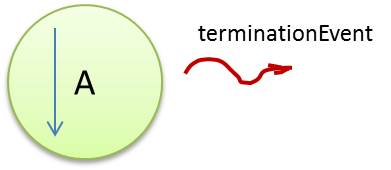
\includegraphics[scale = 0.5]{img/actionObservable.jpg}\\
\end{tabular}{   }
\end{center}
 

\subsection{The class \texttt{ActionObservableGeneric}}
\labelssec{actionObservableGeneric}

The generic, abstract class \texttt{ActionObservableGeneric<T>} provides an implementation support for Observable Actions. It implements the following interface \footnote{The code is included in the file \textit{qactor18.jar}.}  

\lstinputlisting[language=java,caption={ \texttt{IObservableActionGeneric<T>} }, firstline=1 ]{../../../it.unibo.qactor/src/it/unibo/qactors/action/IObservableActionGeneric.java}

The meaning of some important operations is reported in the following table:

\medskip 
\begin{tabular}{|l|l|}
\hline 
\texttt{Future<T> activate()} & starts the action as an asynchronous operation \\ 
\hline 
\texttt{void execAction()} & executes the action and waits for termination \\ 
\hline 
\texttt{long getExecTime()} & returns the execution time of the action \\ 
\hline 
\texttt{String getTerminationEventId()} & returns the name of the termination event\\ 
\hline 
\texttt{String getResultRep()} & returns (a representation of) the result of the action\\ 
\hline 
\end{tabular} 

 

\subsubsection{The interface \texttt{Callable<T>}.\\}
Since an Observable Action is a \texttt{java.util.concurrent.Callable<T>}, it must define the operation \texttt{<T> call()}.
The \texttt{Callable} interface is similar to \texttt{Runnable}, in that both are designed for classes whose instances are potentially executed by another thread. A \texttt{Runnable}, however, \textit{does not return a result} and cannot throw a checked exception.

\subsubsection{The interface \texttt{Future<T>}.\\}
\labelssec{future}

The operation \texttt{activate} starts the execution of the action (see \xss{activate}) and returns an object that must implement the interface \texttt{java.util.concurrent.Future<T>}. 

In \java{}, a \texttt{Future} represents the result of an asynchronous computation. It exposes methods allowing a client to monitor the progress of a task being executed by a different thread. Therefore a Future object can be used to check the status of a \texttt{Callable} and to retrieve the result from the \texttt{Callable}. More specifically:
\begin{itemize}
\item Check whether a task has been completed or not.
\item  Cancel a task.
\item Check whether task was cancelled or complete normally.
\end{itemize}
 
In programming languages, the \textit{future} concept is also known as \textit{promises} or \textit{delays}.


\subsubsection{The operation \texttt{activate}.\\}
\labelssec{activate}

The operation \texttt{activate()} starts the action as an asynchronous operation by using the class \texttt{java.util.concurrent.Executors}
\begin{javacode}
protected Future<T>  fResult;
	public Future<T> activate() throws Exception{
		Result = EventPlatformKb.manyThreadexecutor.submit(this);	
 		return fResult;
 	}
\end{javacode} 

\subsubsection{The class \texttt{Executors}.\\}
\labelssec{future}

Since working with the \texttt{Thread} class can be very tedious and error-prone, the \textit{Concurrency API} has been introduced back in \texttt{2004} with the release of \texttt{Java 5}. The \texttt{API} is located in package \textit{java.util.concurrent} and contains many useful classes for handling concurrent programming, including the concept of an \textit{ExecutorService} as a higher level replacement for working with threads directly. Executors are capable of running asynchronous tasks and typically manage a pool of threads. 

\subsubsection{The operation \texttt{execAction}.\\}
\labelssec{execAction}

The operation \texttt{execAction()} activates the action and forces the caller to waits for the termination of the action execution.

\begin{javacode}
	@Override
	public void execAction() throws Exception {
		activate();
		fResult.get();	//to force the caller to wait
	}
\end{javacode}



\subsubsection{The operation \texttt{T call}.\\}
\labelssec{call}

The operation \texttt{T call()} is the entry point for the Executor and is defined as a sequence of internal operations that starts by taking the current time and ends by calculating the execution time and by emitting the action termination event.

\begin{javacode}
	/* Entry point for the Executor */
	@Override
	public T call() throws Exception {
		startOfAction(); 
		execTheAction();
		result = endActionInternal();
		return result;
	}
\end{javacode}

\subsubsection{The operation \texttt{startOfAction}.\\}
\labelssec{startOfAction} 

The operation \texttt{startOfAction} takes the current time and retains a reference to the current Thread:
\begin{javacode}
protected Thread myself;
	protected void startOfAction() throws Exception{
		tStart = Calendar.getInstance().getTimeInMillis();
		myself = Thread.currentThread();		
	}
\end{javacode}

\subsubsection{The operation \texttt{endActionInternal}.\\}
\labelssec{endActionInternal} is executed when the action is terminated; it evaluates the action execution time and emits the termination event with payload \texttt{result(RES,EXECTIME)}:

The operation \texttt{endActionInternal} 
\begin{javacode}
 	/* Calculate action execution time and emit the termination event */
	protected T endActionInternal() throws Exception{
 		T res = endOfAction();
		emitEvent( terminationEvId, res );
		return res;
	}
	protected void emitEvent(String event, T res){
		long tEnd = Calendar.getInstance().getTimeInMillis();
		durationMillis =  tEnd - tStart ;	
    	platform.raiseEvent( getName(), event, "result("+res+",exectime("+durationMillis+"))" );		
	} 
\end{javacode}

\subsubsection{The operations \texttt{execTheAction} and  \texttt{endOfAction }.\\}
The operations \texttt{execTheAction} and \texttt{endOfAction} are declared \texttt{abstract} in the class \textit{ActionObservableGeneric<T>}. 

\begin{javacode}
	/* TO BE DEFINED BY THE APPLICATION DESIGNER */
	protected abstract void execTheAction() throws Exception; 
	protected abstract T endOfAction() throws Exception; 
\end{javacode}

These operations must be defined by the application designer in the following way:

\medskip 
\begin{tabular}{|l|l|}
\hline 
\texttt{execTheAction} & defines the 'businnes logic' of the action \\ 
\hline 
\texttt{endOfAction} & returns the main result of the action \\ 
\hline 
\end{tabular} 
 
\subsection{Fibonacci as Observable Action}
The \texttt{fibonacci} computation of \xs{aboutactions} is defined in the following as a Observable Action that takes at construction time a goal of the form \texttt{fibo(N,V)} where \texttt{N} is the fibonacci number to evaluate and \texttt{V} is the (variable that denotes the) result

\lstinputlisting[language=java,caption={ \texttt{ActionObservableFibonacci<T>} }, firstline=1 ]{../../../it.unibo.robot.interactive/src/it/unibo/actionobsexecutor/ActionObservableFibonacci.java}

\subsubsection{Experiments on Fibonacci as Observable Action.}

The project \textit{it.unibo.robot.interactive}, package \texttt{it.unibo.actionobsexecutor} shows the effects of the action in the different execution modes:



\begin{center}
\begin{tabular}{ c }
     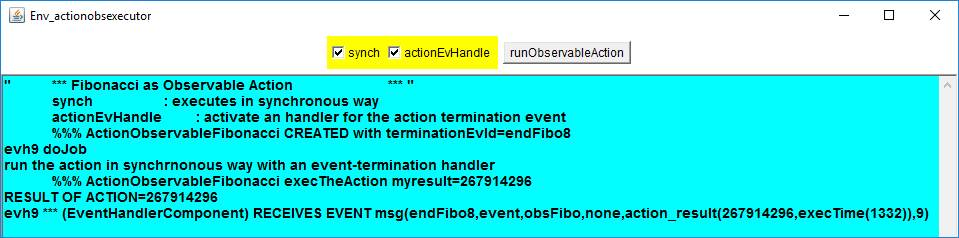
\includegraphics[scale = 0.6]{img/actionObs.jpg}\\
\end{tabular}{   }
\end{center}


 \newpage 
\subsection{Timed actions}
\labelssec{timedAction}

In several situations, an application designer could activate actions that must always terminate within a prefixed amount of time. In \xss{planactions} we have introduced the idea of \textit{timed action}.

We can define an \textit{\textbf{Timed Action}} as an \textit{Observable Action} whose execution time \texttt{T} satisfies the constraint \texttt{T<=DURATION}, where \texttt{DURATION} is a prefixed amount of time\footnote{Usually, \texttt{T} and \texttt{DURATION} are expressed in millisecs.}. Moreover:
\begin{itemize}
\item the action can be activated in two different ways: \textit{synchronous mode} and \textit{asynchronous mode};
\item a Timed Action activated in  \textit{\textbf{synchronous}} mode: \textit{i)} blocks the activator until the action is completed and \textit{ii)} emits a termination event when it ends its work;
\item a Timed Action activated in  \textit{\textbf{asynchronous}} mode:  \textit{i)} returns immediately the control to the activator, \textit{ii)} emits immediately the termination event and \textit{iii)} emits another event (called \textit{\textbf{answer} event}) when it ends its work;
\item a Timed Action can be \textit{\textbf{suspended}} (interrupted) even if it not already terminated. A Timed Action is called \textbf{\textit{recoverable}} if the action can resume its work after a suspension.
\item the \textit{\textbf{result}} of a Timed Action is an object (of type \texttt{AsynchActionGenericResult<T>}, see \xss{AsynchActionGenericResult}) that the wraps the application result into a structure that gives other information about the action (e.g. interrupted or not, execution time remained with respect to the \texttt{DURATION}, etc.)
 \item 
\end{itemize}

Thus, a Timed Action works in its own thread of control; its activator can decide to wait for the termination of the action (\textit{synchronous mode} activation) or to continue its work. In case of \textit{asynchronous mode} activation, an actor interested in the application result of the action can look at the \textit{answer event} emitted by the action. An actor can also suspend an action, and, if the action is recoverable, continue its execution later\footnote{This kind of behaviour is useful for example  when a robot must execute a move for some time, while being able to reacts to alarms.}. 

\subsection{The class \texttt{ActorTimedAction}}
\labelssec{ActorAction} 
The class \texttt{ActorTimedAction} implements the concept of Timed Action by building a 'subsystem' composed of the action and other two components: a timer and a event handler:

%and is the basic building block for the different types of \textit{PlanActions} introduced in \xss{planactions}:

\medskip 
\begin{center}
\medskip 
\begin{tabular}{|c|c|}
\hline 
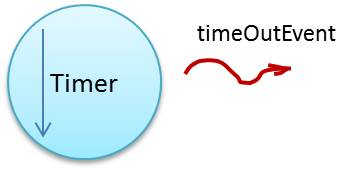
\includegraphics[scale = 0.5]{img/actionTimer.jpg} & 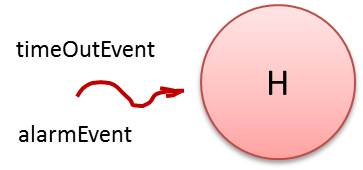
\includegraphics[scale = 0.5]{img/actionEventHandler.jpg} \\ 
\hline 
\end{tabular}
\end{center}

\lstinputlisting[language=java,caption={ \texttt{ActorTimedAction} }, firstline=1 ]{../../../it.unibo.qactor/src/it/unibo/qactors/action/ActorTimedAction.java}

The architecture of the 'subsystem' built by the \texttt{init} operation of \texttt{ActorAction} is shown in the following picture:

\begin{center}
\begin{tabular}{ c }
     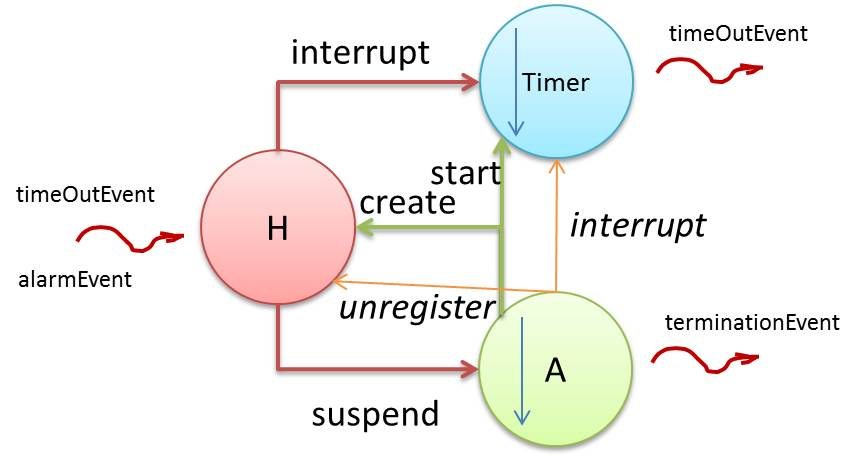
\includegraphics[scale = 0.5]{img/actionTimedReactive.jpg}\\
\end{tabular}{   }
\end{center}




\subsection{The class \texttt{AsynchActionGeneric}}
\labelssec{AsynchActionGeneric}

The generic, abstract class \texttt{AsynchActionGeneric<T>} provides the \texttt{API} for Timed Actions, as defined by the following interface \footnote{The code is included in the file \textit{qactor18.jar}.}  

\lstinputlisting[language=java,caption={ \texttt{IAsynchAction<T>} }, firstline=1 ]{../../../it.unibo.qactor/src/it/unibo/qactors/action/IAsynchAction.java}

The meaning of some important operations is reported in the following table:

\medskip 
\noindent
\begin{scriptsize}
\begin{tabular}{|l|l|}
\hline 
\texttt{AsynchActionGenericResult<T> execSynch()} & executes the action in synchronous way (waits for termination) \\ 
\hline 
\texttt{Future<AsynchActionGenericResult<T>> execAsynch} & executes the action in asynchronous way \\ 
\hline 
\texttt{AsynchActionGenericResult<T> waitForTermination()} & waits until the action is terminated (mainly for execAsynch) \\ 
\hline 
\texttt{void suspendAction()} & suspends the execution of the action if not already terminated \\ 
\hline 
\texttt{ActionRunMode getExecMode()} & returns an instance of ActionRunMode (termination with answer or not) \\  
\hline 
\end{tabular} 
\end{scriptsize}  

\subsection{The class \texttt{AsynchActionGenericResult}}
\labelssec{AsynchActionGenericResult}

The generic class \texttt{AsynchActionGenericResult<T>} provides objects that represent the result of a Timed Action:

\lstinputlisting[language=java,caption={ \texttt{AsynchActionGenericResult<T>} }, firstline=1  ]{../../../it.unibo.qactor/src/it/unibo/qactors/action/AsynchActionGenericResult.java}


\subsection{Fibonacci as a Timed Action}
\labelssec{fibotimed}

The \texttt{fibonacci} computation of \xs{aboutactions} is defined in the following as a Timed Action that takes at construction time a goal of the form \texttt{fibo(N,V)} where \texttt{N} is the fibonacci number to evaluate and \texttt{V} is the (variable that denotes the) result.

\lstinputlisting[language=java,caption={ \texttt{ActionTimedFibonacci<T>} }, firstline=1 ]{../../../it.unibo.robot.interactive/src/it/unibo/actiontimedexecutor/ActionTimedFibonacci.java}

\subsubsection{Experiments on Fibonacci as Timed Action.}

The Project \textit{it.unibo.robot.interactive}, package \texttt{it.unibo.actiontimedexecutor} shows the effects of the action in the different execution modes:
 
\begin{center}
\begin{tabular}{ c }
     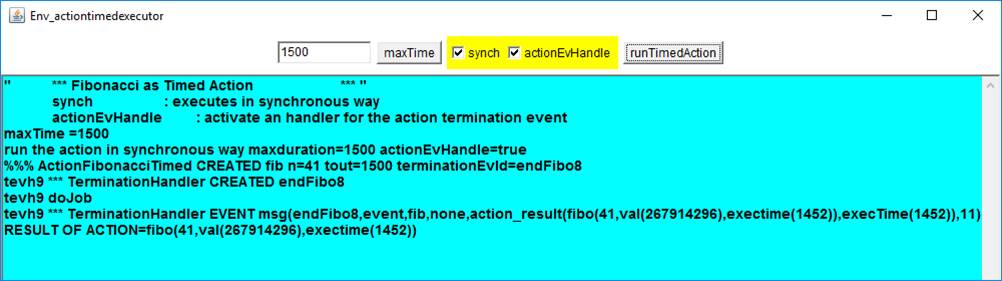
\includegraphics[scale = 0.6]{img/actionTimed.jpg}\\
\end{tabular} 
\end{center}



 \newpage 
\subsection{Reactive actions}
\labelssec{reactiveactions}
We can define a \textit{\textbf{Reactive Action}} as a \textit{Timed Action} that can be suspended (interrupted) by the occurrence of events.  

The occurrence of an event E that suspends the execution of a reactive action RA in a plan P, gives raise to the execution of a plan EP associated to the event E. The plan EP, once terminated, can terminate the behaviour of the Actor or resume the plan P, that will be continue from the suspension point of the action RA, if it is recoverable, or from the action that follows RA in P.

%% The execution of a Reactive Action is done under the control of a \textit{TaskActionFsmExecutor} that is able to handle the action termination-event and any expected 'interruption' event (including a time-out) that can happen while the action is running. 

%%This Reactive Action executor is a specialization of an abstract \texttt{TaskComponent} that implements a event-based finite-state machine whose input-set is called \textit{inputSymbolEventsSet}. The run-time support resumes a Task only when the current event belongs to \textit{inputSymbolEventsSet} and this input is in the \textit{expectedInput} set of its current Task \textit{state}. This work is done by an event handler (of class \textit{TaskQueueEventHandler}) that:
%% \begin{itemize}
%% \item is automatically created when a new Task instance is created
%% \item reacts to all the events that belong to the  \textit{inputSymbolEventsSet} of the Task;
%% \item resumes the Task if it is not already activated;
%% \item stores the event in a local queue if the Task already activated.
%% \end{itemize}

 

\subsection{Fibonacci as a Reactive Action}
\labelsec{fiboreactive}

 
The \texttt{fibonacci} computation of \xss{fibotimed} can be used to build a Reactive Action, by introducing a test to 'interrupt' the action if it has been suspended by some event.

\lstinputlisting[language=java,caption={ \texttt{ActionReactiveFibonacci<T>} }, firstline=1 ]{../../../it.unibo.robot.interactive/src/it/unibo/actionreactiveexecutor/ActionReactiveFibonacci.java}

\subsubsection{Experiments on Fibonacci as Reactive Action.}

The Project \textit{it.unibo.robot.interactive}, package \texttt{it.unibo.actionreactiveexecutor} shows the effects of the action in the different execution modes. When the \texttt{interrupt} flag is set, an event \texttt{usercnd : stop} is generated\footnote{The \texttt{QActor} operation \texttt{emitEventAsynch} performs the task to generate a given event after a given time.} after \texttt{maxtime/2} \textit{msecs}. 


\begin{center}
\begin{tabular}{ c }
     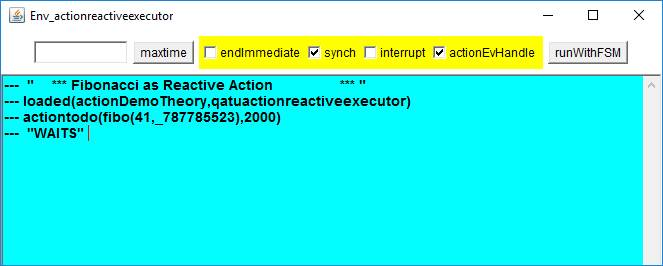
\includegraphics[scale = 0.6]{img/actionReactive.jpg}\\
\end{tabular} 
\end{center}

%% \input{IntroductionQrobots.tex}
%% \section{The problem}
We have to solve to following problem:
 
\medskip 
\scriptsize
\framebox[15cm]{ %
\begin{minipage}{140mm}
Build a distributed system composed of a Button and a Led, each controlled by a different computational node.
The system must initially provide a very basic function: a Led is turned on and off each time a Button is pressed (by an human user). 

In the future, the functionalities of the systems could be extended, e.g. by allowing a Button to blink a Led, to turn on/off many Led etc.
\end{minipage}}
\normalsize
\medskip    

We read the text file that describes the requirements and immediately plan some work to:

\begin{itemize}
\item define the model of the Led (question: \textit{what} is a Led in the user domain space?);
\item define the model of the Button (question: \textit{what} is a Button in the user domain space?);
\item define the (model of the) Use Cases (i.e. define the functions/features of the software system).
\end{itemize}

\subsection{The UseCases.}
The main functions of the software systems can be summarized as done in
\href{https://137.204.107.21/syskb/it.unibo.iss2015intro/docs/Appls/ButtonLed/buttonLedHighLevelEntry.html}{|>>site/BLS usecases}.

\subsection{From Requirement Analysis to the software development process}

After the analysis related to the system components, we ask ourselves whether the models of the Led and of the Button defined in cooperation with the user can be also suited to face the problem of building the required distributed software system. Since it is not the case, we immediately advert a conceptual distance between the basic components and the needs of the application (i.e. we find an \textit{abstraction gap}) that can be reduced by describing the single components and the whole system by means of a custom meta-model, no more based on classical objects but on \textit{actors}.

In the following, we will show how a proper requirement analysis staring from the system components, properly related to the problem analysis and formally expressed by (executable) models can provide a solid guide for agile (\texttt{SCRUM}-based) project and implementation phases by reducing the risks and the costs for the software company.

\newpage 
\section{The Led (as basic logical device)}
\labelsec{led}
In the application domain of the customer, the Led is a physical device (see
\href{https://137.204.107.21/syskb/it.unibo.iss2015intro/docs/Appls/ButtonLed/LedEntry.html}{|>>site/LedEntry}) that can be modelled  as a \textit{Plain Old Java Object} (see \href{https://en.wikipedia.org/wiki/Plain_Old_Java_Object}{net/POJO} ).


\subsection{The Led as a \texttt{POJO}}
%
More precisely, we can state that a Led is an object with a modifiable state that can provide (implement) the following interface:

%%\begin{Verbatim}[fontsize=\scriptsize, frame=single]
\begin{lstlisting}
public interface ILed {
  public String getName();             // property , primitive	
  public void turnOn();                // modifier , primitive
  public void turnOff();               // modifier , primitive
  public java.awt.Color getLedColor(); // property , primitive
  public boolean isOn();               // property , primitive
  public void doSwitch();              // non-primitive
  public String getDefaultRep();       // mapping , non-primitive
}
\end{lstlisting}
%%\end{Verbatim}

The comments near each operation give some first indication on the intended semantics of the operation according with the terminology reported in \href{https://137.204.107.21/syskb/it.unibo.iss2015intro/docs/NatMolBook/content/book/sistemi/comportamentoSistemi.html}{book/ops	})

%% \lstinputlisting[language=java,caption={ \texttt{ILed.java} }, firstline=1 ]{../../../it.unibo.buttonLedSystemHL/src/it/unibo/bls/lowLevel/interfaces/ILed.java}

%% \lstinputlisting[language=java,caption={ \texttt{IDeviceLedImpl.java} }, firstline=1 ]{../../../it.unibo.buttonLedSystemHL/src/it/unibo/bls/lowLevel/interfaces/IDeviceLedImpl.java}

%% At the very first stage of development, the \texttt{ILed} interface and the  is introduced without any need to define a \texttt{IDeviceLedImpl}. However, since our software company is working in the \texttt{IOT} (\textit{Internet of Things}) filed, it has already defined a reusable taxonomy for \texttt{IOT} devices, according to the model discussed in \xss{devbridge}.

\subsection{The Led model test-plan}
\labelssec{ledtestplan}
However, the usage of comments is not the best way to specify the intended semantics of an operations.
By recalling the motto of Young et al. (1985):

\medskip 
\scriptsize
\framebox[15cm]{ %
\begin{minipage}{140mm}
A design without specifications cannot be right or wrong, it can only be surprising! 
\end{minipage}}
\normalsize
\medskip 


our next step is to immediately introduce a test plan (see  \href{https://137.204.107.21/syskb/it.unibo.iss2015intro/docs/NatMolBook/content/book/modelBased/fasi/pianoCollaudo.html}{book/test plans}), to better specify the expected  behaviour (i.e. the meaning) of each operation.

The test plan that follows is directly expressed in \texttt{JUnit} (see 
\href{http://www.vogella.com/tutorials/JUnit/article.html}{net/JUnit tutorial}) even if we do not have, at this moment, nothing to test. The idea is to use each test as a \textit{specification} of the expected behaviour and as a way to express in a more formal way what each operation should do.

\lstinputlisting[language=java,caption={ \texttt{A Test Plan for the Led} }, firstline=1 ]{../../../it.unibo.buttonLedSytem.tests/src/it/unibo/buttonLedSytem/tests/TestLed.java}

%%\href{https://137.204.107.21/syskb/it.unibo.iss2015intro/docs/NatMolBook/Testing.html}{testing}), to better specify the expected behaviour of each Led operation:

\subsection{The Led as an actor (problem analysis)}
\labelssec{ledasactor}
The current model of the Led as a \texttt{POJO} does not include any capability to interact via the network  with the other components of the system. In other words, this model is not able to capture the distributed nature of the system.

In the context of a distributed button-led system, the Led could be conceived as a more advanced device, modelled as an \textit{actor} able to receive and execute command messages. 
%
This new model can be expressed by using the \texttt{qa} metamodel as follows:
\lstinputlisting[language=ddr,caption={ \texttt{ledMsg.qa} }, firstline=1 , lastline=31]{../../../it.unibo.bls2016.led/src/ledMsg.qa}

The \texttt{ledmsg} actor is a state machine that first performs a configuration phase and then works in a message-based way.
% 
In the configuration phase the actor load a theory (\texttt{ledTheory}) and creates a (\texttt{POJO}) Led, that will be updated by calling \tuprolog{} rules (\texttt{turnTheLed/1} or \texttt{turnOn/turnOff}) defined in the \texttt{ledTheory}.

Thus, the idea of a Led as a \texttt{POJO} is not abandoned; it is simply included (embedded) into the more advanced concept of \texttt{ledmsg} actor.

\subsection{The Led (configuration) \texttt{ledTheory} }
\labelssec{ledTheory}
The main task of the \texttt{ledTheory} is done during its \textit{initialization}: load a specific led-theory for each Led implementation:

\lstinputlisting[language=ddr,caption={ \texttt{ledTheory.pl} }, firstline=1 ]{../../../it.unibo.bls2016.led/ledTheory.pl}

If no \texttt{ledImplementation/1} fact is defined within the \texttt{ledTheory}, then we do not have any concrete Led implementation to use, as usually happens during the requirement or problem analysis phase. Nevertheless, we aim at introducing a working model even in this early phase of software development, in order to better interact with the user and to fix the requirements as soon as possible. For this reason the \texttt{ledTheory} loads a \texttt{ledNoImplTheory}. 

\subsection{A first Led (implementation) object}

The \texttt{ledNoImplTheory}  models the led state as a fact \texttt{ledState/1} and 'implements' the Led operations by introducing a proper set of rules:

 
%% The \texttt{ledTheory} is introduced to link the abstract view of the Led as an actor to some 'concrete' device (object), implemented with some specific technology; for example, we could introduce a physical Led controlled by an Arduino or a Raspberry or a virtual Led implemented by a GUI, and so on. 

%% However, when we are in the requirement or problem analysis phase, we should avoid to enter in any technological detail at this stage; nevertheless, we aim at introducing a working model even in this early phase of software development, in order to better interact with the user and to fix the requirements as soon as possible.

%% For this reason we model the led state as a fact \texttt{ledState/1} and 'implement' the Led by introducing a proper set of rules. 

\lstinputlisting[language=ddr,caption={ \texttt{ledNoImplTheory.pl} }, firstline=1 ]{../../../it.unibo.bls2016.led/ledNoImplTheory.pl}

This theory defines a very simple implementation of the Led as a \texttt{POJO}, by introducing rules related to the \texttt{ILed} interface of \xss{ledtestplan}. 


In this way, we are able to build a working prototype of a basic component (and later of the whole system) in a short time still during requirement analysis; even the unit test plans of \xss{ledtestplan} can be included in the component prototype.

The \texttt{createLed/2} rule is by now defined by asserting some facts in the knowledge base. This rule will be proprerly re-defined in each specific Led implementation theory, in order to introduce a specific concrete device, for example the \texttt{LedMock} used in the test plan of \xss{ledtestplan}.
 
%%Since we can have several Led implementation, we associate a theory to each type of Led implementation and use a rule to detect and load the proper theory:

%%\lstinputlisting[language=ddr,caption={ \texttt{ledTheory.pl} }, firstline=1 ]{../../../it.unibo.bls2016.led/ledTheory.pl}

\subsection{Testing the actor Led component} 
The Led component model can be executed by adding in the \texttt{qa} model a simple message generator (that will be later replaced by a button or by some other input  device):
\lstinputlisting[language=ddr,caption={ \texttt{ledMsg.qa extended with a Led command generator } }, firstline=32 ]{../../../it.unibo.bls2016.led/src/ledMsg.qa}

\subsection{A Mock Led (project/implementation phase)}
\labelssec{ledmock}

Our software company has already developed an implementation for a mock object\footnote{In object-oriented programming, \textit{mock objects} are simulated objects that mimic the behaviour of real objects in controlled ways.}  for the Led :

\lstinputlisting[language=java,caption={ \texttt{LedMock.java} }, firstline=1 ]{../../../it.unibo.buttonLedSystemHL/src/it/unibo/buttonLed/components/LedMock.java}

Since this class is the result of some project or implementation phase, a lot of work has been already done to enhance code reusability. In particular, the software team has introduced the class \texttt{DeviceLedImpl} (see  \xss{DeviceLedImpl} ) as a basic class for all the different types of Led implementations; in this way, for each specific Led implementation we have to redefine some operation only (in this case the internal operation \texttt{show}). 

In order to 'inject' this new implementation of the Led into our logical component, we define the theory \texttt{ledMockTheory} with a specific \texttt{createLed/2} rule: 


\lstinputlisting[language=ddr,caption={ \texttt{ledMockTheory.pl} }, firstline=1 ]{../../../it.unibo.bls2016.led/ledMockTheory.pl}

The next step is to introduce two new rules in  the \texttt{ledTheory} of \xss{ledTheory}:

%%\begin{Verbatim}[fontsize=\scriptsize, frame=single , label=Facts related to \texttt{LedMock} in \texttt{ledTheory	}]
\begin{lstlisting}
ledImplementation( mock ).
...
ledImplementationFile( mock, "ledMockTheory.pl"   ).
\end{lstlisting}
%%\end{Verbatim}

\newpage 
\section{A Led factory }
\labelssec{DeviceLedFactoryQa}
The \java{} class \texttt{DeviceLedFactoryQa} used in the \texttt{LedMock} of \xss{ledmock} is a \textit{factory} that provides static methods to create a \textit{singleton} Led object and to get a reference to such an object:

\lstinputlisting[language=java,caption={ \texttt{DeviceLedFactoryQa.java : createLedMock} }, firstline=1 , lastline=25]{../../../it.unibo.bls2016.device.qa/src/it/unibo/devices/qa/DeviceLedFactoryQa.java}

Note that the creation method \texttt{createLedMock} returns (like any other creation method that we will introduce in the factory) an object of the class \texttt{DeviceLedImpl} (see  \xss{DeviceLedImpl} ). 

\subsection{The Led usage theory }
Since we have introduced a factory that builds and gets objects of class  \texttt{DeviceLedImpl}, we can write a set of Led-usage rules that do not depend on the specific Led implementation:

\lstinputlisting[language=ddr,caption={ \texttt{ledUsageTheory.pl} }, firstline=1 ]{../../../it.unibo.bls2016.led/ledUsageTheory.pl}

\subsection{A basic class for Led implementation}
\labelssec{DeviceLedImpl}
The \texttt{DeviceLedImpl} class is based on the custom framework \href{https://137.204.107.21/syskb/it.unibo.iss2015intro/docs/Frameworks/FramwCustomAppl.html}{|>>site/uniboEnv}) introduced for the rapid development of \texttt{GUI}-based prototypes.

\lstinputlisting[language=java,caption={ \texttt{DeviceLedImpl.java} }, firstline=1 ]{../../../it.unibo.buttonLedSystemHL/src/it/unibo/buttonLed/components/DeviceLedImpl.java}


\subsection{A Virtual Led (project/implementation phase)}

A Led as a virtual device can now be introduced as follows:

%%\lstinputlisting[language=java,caption={ \texttt{DeviceLedGui.java} }, firstline=1 ]{../../../it.unibo.buttonLedSystem.gui/src/it/unibo/buttonLedSystem/gui/DeviceLedGui.java}

The class  \texttt{DeviceLedImpl} redefines two internal operations: \texttt{configure} and \texttt{show}. The result is shown in the following picture:

%%This implementation is a specialized version of the more general Led implementation class (\texttt{DeviceLedImpl},see  \xss{DeviceLedImpl} ) that changes the size of a picture when the Led changes its state.

\begin{center}
\begin{tabular}{ c }
     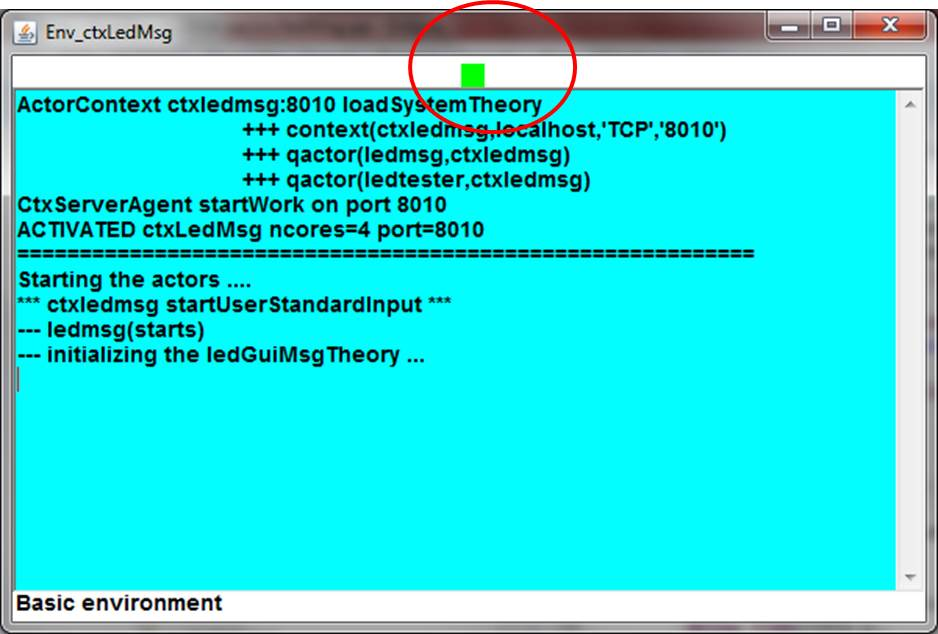
\includegraphics[scale = 0.45]{./img/ledGui.jpg}\\
\end{tabular}{   }
\end{center}

In order to 'inject' this new implementation of the Led into our logical component, we define the theory \texttt{ledGuiTheory} with a specific \texttt{createLed/2} rule: 


\lstinputlisting[language=ddr,caption={ \texttt{ledGuiTheory.pl} }, firstline=1 ]{../../../it.unibo.bls2016.led/ledGuiTheory.pl}

The next step is to introduce two new rules in  the \texttt{ledTheory} of \xss{ledTheory}:

%%\begin{Verbatim}[fontsize=\scriptsize, frame=single , label=Facts related to \texttt{LedGui} in \texttt{ledTheory	}]
\begin{lstlisting}
ledImplementation( gui ).
...
ledImplementationFile( gui,  "ledGuiTheory.pl"   ).
\end{lstlisting}
%%\end{Verbatim}
 
Finally, we introduce a new Led creation operation in the entry in the \texttt{DeviceLedFactoryQa}:
\begin{lstlisting}
    public static DeviceLedImpl createLedGui(  
    		 String name, IOutputEnvView outEnvView, int color) throws Exception{
     	if( myself == null ){
  	  		LedColor ledcolor = (color == 0) ? LedColor.GREEN : LedColor.RED ;
	  		myself = new DeviceLedGui(name,outEnvView, ledcolor);  			 
  		}
  		return myself;
   	}
\end{lstlisting}
\newpage 
\section{A Led on Raspberry (implementation phase)}
The \texttt{GPIO} pins on a Raspberry Pi are a great way to interface physical devices like Buttons and Leds through some simple hardware connection, as in the example described in
%\href{https://137.204.107.21/syskb/it.unibo.iss2015intro/docs/Raspberry/pi4j.html}{|>>site/Pi4j}) and 
\href{https://137.204.107.21/syskb/it.unibo.iss2015intro/docs/Appls/ButtonLed/buttonLedLowLevel.html}{|>>site/BLS low-level})). In this example the Led anode  is connected to pin \texttt{25} in \texttt{BCM} code\footnote{\texttt{BCM} refers to the pin number of the \texttt{BCM2835} chip, and this is the pin number used when addressing the \texttt{GPIO} using the \texttt{/sys/class/gpio} interface}  while the Led cathode is connected to a \texttt{GND} pin.

However, a software design never interacts in direct way with the hardware level; at least some minimal support for the control of external devices must be provided by the operating system. In the case of Linux we can start from the shell or from a more advanced library.


\subsection{Led control using files}
The basic way provided by Linux to manage a device connected on a \texttt{GPIO} pin is reading/writing some (virtual) file associated with that pin.

\lstinputlisting[language=ddr,caption={ \texttt{led25OnOff.sh} }, firstline=1 ]{../../../it.unibo.raspIntro/src/it/unibo/bls/bash/led25OnOff.sh}

\subsection{Led control using the \texttt{GPIO} shell library}
\textit{WiringPi} is a \texttt{GPIO} access library written in \texttt{C}\footnote{The \textit{WiringPi}  library was written by Gordon Henderson to allow \texttt{GPIO} communication from \texttt{C,C++} in a style similar to the Arduino Wiring programming language} for the \texttt{BCM2835} used in the Raspberry Pi. \textit{WiringPi} includes a command-line utility \texttt{gpio} which can be used to program and setup the \texttt{GPIO} pins. We can use this to read and write the pins and even use it to control them from shell scripts.

\lstinputlisting[language=ddr,caption={ \texttt{led25Gpio.sh} }, firstline=1 ]{../../../it.unibo.raspIntro/src/it/unibo/bls/bash/gpio/led25Gpio.sh}

\subsection{Led control using python}
The Raspbian Linux operating system  has the \texttt{RPi.GPIO} library pre-installed. It is a Python library that handles interfacing with the \texttt{GPIO} pins.

\lstinputlisting[language=ddr,caption={ \texttt{ledPython25.sh} }, firstline=1 ]{../../../it.unibo.raspIntro/src/it/unibo/bls/python/ledPython25.py}

 \subsection{Led control using Pi4j}
\texttt{Pi4J} is an open source project  intended to provide a bridge between the native hardware and \java{} for full access to the Raspberry Pi. In addition to the basic raw hardware access functionality, this project also attempts to provide a set of advanced features that make working with the Raspberry Pi an easy to implement and more convenient experience for \java{} developers.

Thus, the \texttt{Pi4J} library (see \href{https://137.204.107.21/syskb/it.unibo.iss2015intro/docs/Raspberry/pi4j.html}{|>>site/Pi4j}) can be used as our basic software layer (our \textit{technology assumption}) for the implementation a \java{} class for the control of a Led connected to some pin of a Raspberry Pi:

\lstinputlisting[language=java,caption={ \texttt{DeviceLedPi4j.java} }, firstline=1 , lastline=50]{../../../it.unibo.buttonLedSystem.raspberry/src/it/unibo/bls/raspberry/components/DeviceLedPi4j.java}

In this case the class redefines two primitive operations of \texttt{DeviceLedImpl} (see \xss{DeviceLedImpl}): \texttt{turnOn} and \texttt{turnOff}. Moreover, it extends the configuration phase by 'provisioning' (in \texttt{Pi4j} terminology) the \texttt{GPIO} pin connected to the Led anode. 
%
The class \texttt{GpioOnPi4j} is an utility class that maps a \texttt{GPIO} pin number in \texttt{BCM}  into a \textit{wiring Pi} code:

\lstinputlisting[language=java,caption={ \texttt{GpioOnPi4j.java} }, firstline=1 , lastline=54]{../../../it.unibo.bls2016.device.qa/src/it/unibo/gpio/base/GpioOnPi4j.java}

\subsection{Using the Led Pi4j in the actor}
In order to 'inject' this new implementation of the Led into our logical component, we define the theory \texttt{ledPi4jTheory.pl}:

\lstinputlisting[language=ddr,caption={ \texttt{ledPi4jTheory.pl} }, firstline=1 ]{../../../it.unibo.bls2016.led/ledPi4jTheory.pl}

The next step is to introduce two new rules in  the \texttt{ledTheory} of \xss{ledTheory}:

%%\begin{Verbatim}[fontsize=\scriptsize, frame=single , label=Facts related to \texttt{LedMock} in \texttt{ledTheory	}]
\begin{lstlisting}
ledImplementation( rasp ).
...
ledImplementationFile( rasp, "ledPi4jTheory.pl"  ).
\end{lstlisting}
%%\end{Verbatim}

Finally, we introduce a new Led creation operation in the entry in the \texttt{DeviceLedFactoryQa}:
\begin{lstlisting}
    public static DeviceLedImpl createLedPi4j( 
    		 String name, IOutputEnvView outEnvView, int color, int pinNum) throws Exception{
      	if( myself == null ){
    		LedColor ledcolor = (color == 0) ? LedColor.GREEN : LedColor.RED ;
  	  		myself = new DeviceLedPi4j( name,outEnvView, ledcolor, pinNum);  			 
   		}
   	    return myself;
    }
\end{lstlisting}

\subsection{Code deployment on the Raspberry Pi}
In order to test our code on the Raspberry Pi we have to perform the following actions:
\begin{enumerate}
\item create a runnable \texttt{jar} file from the generated file \texttt{src-gen/it/unibo/ctxLedMsg/MainCtxLedMsg.java}\footnote{We suggest to copy the required libraries in a sub-folder to keep the \texttt{jar} short and to reduce the time of file transfer to the Raspberry Pi.};
\item copy the runnable \texttt{jar} and the library sub-folder into a directory (e.g. \texttt{ledTest}) the Raspberry Pi;
\item copy the generated \texttt{scrMore} directory into \texttt{ledTest};
\item copy the into \texttt{ledTest} the theories  \texttt{ledTheory.pl}, \texttt{ledMockTheory.pl}, \texttt{ledGuiTheory.pl} \texttt{ledPi4jTheory.pl} and \texttt{ledUsageTheory.pl}.
\end{enumerate}

\subsection{Test the Led on the Raspberry Pi}
The behaviour of the Led component on the Raspberry Pi can be tested by launching (within the directory \texttt{ledTest}):

\begin{Verbatim}[fontsize=\scriptsize, frame=single , label=Launch the Led test]
sudo java -jar MainCtxLedMsg
\end{Verbatim}

We can select one of the different Led implementations by setting one of the \texttt{ledPi4jTheory.pl} implementation rules:

\begin{Verbatim}[fontsize=\scriptsize, frame=single , label=Select the Led implementation]
%% ledImplementation( mock ).
%% ledImplementation( gui ).
ledImplementation( rasp ).
\end{Verbatim}

The system with the rule \texttt{ledImplementation( gui )} works only under a \texttt{X11} system\footnote{The\textit{ X Window System} (\texttt{X11}, or shortened to simply \texttt{X}, and sometimes informally \texttt{X-Windows}) is a windowing system for bitmap displays, common on \texttt{UNIX}-like computer operating systems} to enable remote graphical access to applications.

\subsection{The Led as a standalone device}
Since we now have a Led working on a Raspberry Pi, we can immediately switch from a local system to a distributed one. To this end, let us introduce an actor that, working on a conventional \texttt{PC}, sends command messages to the Led on the Raspberry Pi:

\lstinputlisting[language=ddr,caption={ \texttt{ledSenderMsg.qa} }, firstline=1 , lastline=31]{../../../it.unibo.bls2016.led/src/ledSenderMsg.qa}

Note that the \texttt{ledtester} is identical to the actor introduced in  \xss{ledasactor}, with the difference that it works in its own Context \texttt{ctxLedSenderMsg}. Moreover, the behaviour of the \texttt{ledmsg} actor is \textbf{not} explicitly defined; rather a 'place holder' actor is introduced in the specification in order to:
\begin{enumerate}
\item allow us to reference the \texttt{ledmsg} actor in a message send (\texttt{forward}) operation;
\item define the context (in practice, the \texttt{IP} of the Raspberry Pi) in which the \texttt{ledmsg} is working.
\end{enumerate}

The flag \texttt{-standalone}  indicates that the Led context \texttt{ctxLedMsg} must be considered an entity outside the system and that the actors defined in it are just 'place holders' that do not produce any new code. More on this in \xs{dynsys}.

 
\newpage 
\section{A Led on Arduino (implementation phase)}
The basic way provided by Arduino to manage a device connected on a pin is to perform a read or a write operation on that pin. For example we can blink a Led connected on pin \texttt{13} as follows:

\lstinputlisting[language=java,caption={ \texttt{Led13.ino}}, firstline=1  ]{../../../it.unibo.arduino.intro/Arduino/programs/Led13/Led13.ino} 

\subsection{Led with input output} 

The next \textit{sketch} does introduce a \texttt{cmdHandler} operation that looks at the serial line as an input device and turns the Led \texttt{on/off} if the input value is \texttt{1/0}.

\lstinputlisting[language=java,caption={ \texttt{Led13Msg.ino}}, firstline=1  ]{../../../it.unibo.arduino.intro/Arduino/programs/Led13Msg/Led13Msg.ino} 



\subsection{DeviceLedArduinoProxy} 
The possibility to send/receive information via the Serial Line can be used as our basic software layer (our \textit{technology assumption}) for the implementation a \java{} class for the control of a Led connected to some pin of a Arduino device. To achieve the goal let us introduce a new specialized version of the \texttt{DeviceLedImpl} (see \xss{DeviceLedImpl}) class:


\lstinputlisting[language=Java,caption={ \texttt{DeviceLedArduinoProxy.java} }, firstline=1 ]{../../../it.unibo.bls2016.device.qa/src/it/unibo/devices/qa/DeviceLedArduinoProxy.java}

The class \texttt{DeviceLedArduinoProxy}\footnote{In computer programming, the \textit{proxy} pattern is a design pattern. A proxy, in its most general form, is a class functioning as an interface to something else.} redefines two primitive operations: \texttt{turnOn} and \texttt{turnOff}. 
%
Moreover, it extends the configuration phase by creating an object of interface \texttt{IConnInteraction} in order to use the serial connection with Arduino.\footnote{The \textit{Java Simple Serial Connector} (\texttt{jscc}) library  is required. It is an evolution of \texttt{RxTx}, see \href{https://blogs.oracle.com/jtc/entry/java_serial_communications_revisited}{net/jSSC}.} 

\subsection{IConnInteraction interface} 
The interface \texttt{it.unibo.is.interfaces.protocols.IConnInteraction} defines operations to send/receive Strings over a  network connection.

\lstinputlisting[language=java,caption={ \texttt{IConnInteraction.java} }, firstline=1 ]{../../../it.unibo.interfaces/src/it/unibo/is/interfaces/protocols/IConnInteraction.java}

The project \textit{it.unibo.noawtsupports} defines a framework for network communications based on connected, two-way protocols (like \texttt{TCP}, \texttt{UDP}) and over a serial line.

The factory \texttt{it.unibo.supports.FactoryProtocol} creates objects of type \texttt{IConnInteraction} that hide the technological details related to specific protocols.  More information on this framework can be found in \href{https://137.204.107.21/syskb/it.unibo.iss2015intro/docs/Readings/UniboSupports/UniboSupports.pdf}{book/UniboSupports.pdf}.

\subsection{Using the serial line in the actor}
In order to 'inject' this new implementation of the Led into our logical component, we define the theory \texttt{ledSerialTheory.pl}:

\lstinputlisting[language=java,caption={ \texttt{ledSerialTheory.pl} }, firstline=1 ]{../../../it.unibo.bls2016.led/ledSerialTheory.pl}

The next step is to introduce two new rules in  the \texttt{ledTheory} of \xss{ledTheory}:

%%\begin{Verbatim}[fontsize=\scriptsize, frame=single , label=Facts related to \texttt{LedMock} in \texttt{ledTheory	}]
\begin{lstlisting}
ledImplementation( serial ).
...
ledImplementationFile( serial, "ledSerialTheory.pl"  ).
\end{lstlisting}
%%\end{Verbatim}

Finally, we introduce a new Led creation operation in the entry in the \texttt{DeviceLedFactoryQa}:
\begin{lstlisting}
    public static DeviceLedImpl createLedSerialProxy( 
   		 String name, IOutputEnvView outEnvView, int color, String portName) throws Exception{
       	if( myself == null ){
       		LedColor ledcolor = (color == 0) ? LedColor.GREEN : LedColor.RED ;
 	  		myself = new DeviceLedArduinoProxy( name, ledcolor, portName, outEnvView);  				 
  		}
       	return myself;
   }
\end{lstlisting}

\newpage 
\section{The Led controlled via a Web page}
\labelsec{ledWeb}
In the \texttt{qa} model of the Led, the flag \texttt{-httpserver} can be introduced in a Context declaration to specify that it must provide a built-in support for web-based interaction. 

\lstset{language=ddr}
\begin{lstlisting}
/*
 * ledMsg.qa
 * This is A MODEL defined during REQUIREMENT or PROBLEM ANALYSIS 
 * by using the qa CUSTOM meta-model / language
 */       
System ledMsg -regeneratesrc      
Dispatch turnLed   : turnLed(X)

Context ctxLedMsg ip [host="localhost" port=8010] -g cyan   -httpserver
...
\end{lstlisting}
\lstset{language=java}

%% \subsubsection{The generated HttpServer.}
When the \texttt{-httpserver} flag is set, a simple \texttt{HTTPserver}\footnote{The class of the server is \texttt{it.unibo.qactors.web.QActorHttpServer})}  is created and started during the Context configuration phase. This server  is based on the \texttt{WebSocket} technology \footnote{The \textit{WebSocket} specification defines an \texttt{API} establishing "socket" connections between a web browser and a server, i.e. a persistent client-server connection so that  both parties can start sending data at any time.} and answers to \texttt{HTTP} requests on port \texttt{8080} by returning the web page named \texttt{QActorWebUI.html} stored in the context package generated in the \texttt{srcMore} directory. 

\subsection{The default page} 
The built-in page has the following aspect:

\begin{center}
\begin{tabular}{ c }
     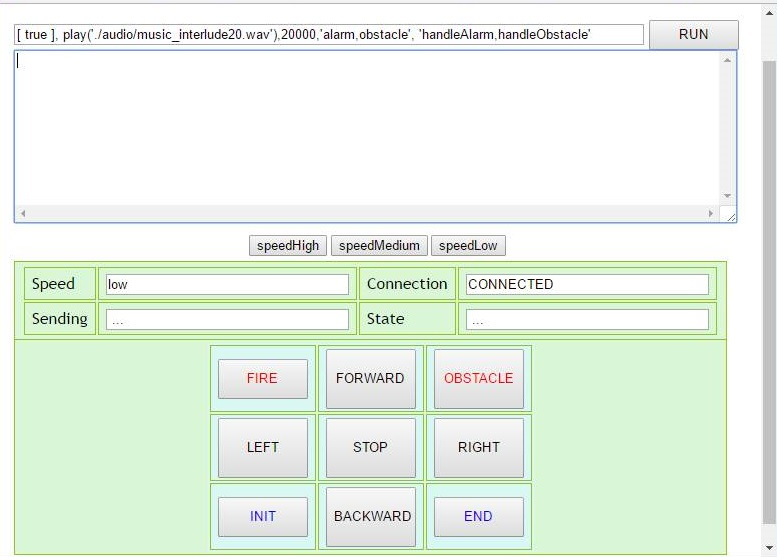
\includegraphics[scale = 0.60]{img/guiweb.jpg}\\
\end{tabular}{   }
\end{center}

The application designer can define (and modify) the content of the \texttt{QActorWebUI.html}  page in order to interact with a QActor by exploiting a conventional Web Browser.

\subsection{A \texttt{HTML} page for the Led}
Let us define a simple page for Led control:

\lstinputlisting[language=ddr,caption={ \texttt{QActorWebUI.html} for the Led }, firstline=1 ]{../../../it.unibo.bls2016.led/descr/QActorWebUI.html}

The page shows itself as follows:
 
\begin{center}
\begin{tabular}{ c }
     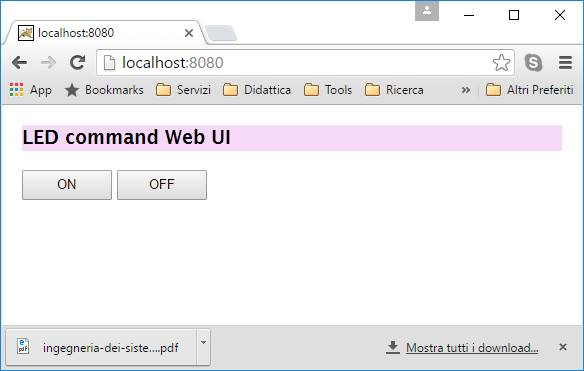
\includegraphics[scale = 0.45]{./img/ledWebGui.jpg}\\
\end{tabular}{   }
\end{center}

The new page for the Led defines two buttons that, once clicked, invoke the \textit{send} operation defined in the \texttt{JavaScript} file \texttt{QActorWebUI.js}:
\lstinputlisting[language=ddr,caption={ \texttt{QActorWebUI.js} for the Led }, firstline=1 ]{../../../it.unibo.bls2016.led/descr/QActorWebUI.js}


\subsection{The work of the built-in QActorHttpServer.} 
 
The \texttt{QActorHttpServer} server handles the input string as follows: 

\lstinputlisting[language=java,caption={ \texttt{QActorHttpServer.java} for the Led }, firstline=156, lastline=165 ]{../../../it.unibo.qactor/src/it/unibo/qactors/web/QActorHttpServer.java} 

Thus, the server performs different actions according to the input string prefix.

\subsection{Input string prefix \texttt{\textbf{m-}}} 
In this case the rest of the input string is assumed to be a \texttt{qa} message of the form:
\medskip
%%\begin{Verbatim}[fontsize=\scriptsize, frame=single , label=]
\begin{lstlisting}
msg( MSGID, MSGTYPE, SENDER, RECEIVER, CONTENT, SEQNUM )
\end{lstlisting}
%%\end{Verbatim}
The \texttt{QActorHttpServer} sends the message to the \texttt{RECEIVER} actor.

For the default page, there no case of this type, that is instead present in the Led web page.

\subsection{Input string prefix \texttt{\textbf{i-}}} 
In this case the rest of the input string is assumed to be a user command (\texttt{CMD}) that is translated into a string of the form:
\medskip   
\begin{Verbatim}[fontsize=\scriptsize, frame=single , label=]
usercmd( executeInput( MOVE ) )
\end{Verbatim}
where \texttt{MOVE} can take one of the following forms:
\medskip
\begin{Verbatim}[fontsize=\scriptsize, frame=single , label=]                                  
[ GUARD ] , ACTION
[ GUARD ] , ACTION , DURATION
[ GUARD ] , ACTION , DURATION , ENDEVENT
[ GUARD ] , ACTION , DURATION , [EVENTLIST], [PLANLIST]
\end{Verbatim}
For the default page, this is the case of the user-command interface; the  \texttt{QActorHttpServer}  emits the following event:

\indent{     } \texttt{usercmd : usercmd(executeInput( CMD ))}	(\texttt{RUN} button) \\

\subsection{Input string without special prefix} 
In this case, the string is assumed to be written in \prolog{} syntax. For the default page, this is the case of the robot-console buttons, that generate input strings of the form:

\begin{Verbatim}[fontsize=\scriptsize, frame=single , label=]
e(alarm(fire))
e(alarm(obstacle))
w( high )
...
\end{Verbatim}
The  \texttt{QActorHttpServer}  emits the following events:  

%% \indent{     } \texttt{inputcmd : usercmd(executeInput( CMD ))} (\texttt{INPUT} button) \\
\indent{     } \texttt{usercmd : usercmd(robotgui(MOVE))} with \texttt{MOVE=w(low),...,s(high)} (\texttt{MOVE} button) \\
\indent{     } \texttt{alarm   : alarm(fire)}  		(\texttt{FIRE} button) \\
\indent{     } \texttt{alarm   : alarm(obstacle)}		(\texttt{OBSTACLE} button)  
 
 
\newpage 
\section{The Button}
\labelsec{button}

As regards the Button, we will follow a  workflow similar to that introduced for the Led in \xs{led} :

\begin{enumerate}
\item model the basic idea of a Button as a \texttt{POJO} component;
\item model the idea of Button required by the problem as an actor;
\item introduce a set of different implementations for the basic button and use them in the proper concrete situation.
\end{enumerate}

\subsection{The Button as a \texttt{POJO}}
\labelssec{ButtonPojo}

In the application domain of the customer, the Button is a physical input device that can be modelled in several ways (a first discussion can be read in \href{https://137.204.107.21/syskb/it.unibo.iss2015intro/docs/Appls/ButtonLed/button.pdf}{|>>site/button.pdf}). 

In this section we start form the idea that a Button is an \textit{observable} (in sense of \texttt{GOF} patterns) \texttt{POJO}.\footnote{See \href{https://137.204.107.21/syskb/it.unibo.iss2015intro/docs/Appls/ButtonLed/buttonEntry.html}{|>>site/buttonEntry}}.
 
%%\subsubsection{The \texttt{IButton} interface.\\}
The Button is then modelled as an entity with some internal modifiable state that can be inspected by all the registered observers or by using the operation \texttt{isPressed}.

%%\begin{Verbatim}[fontsize=\scriptsize, frame=single]
\begin{lstlisting}
public interface IButton {
  public String getName();              // property , primitive	
  public void ispressed();              // property , primitive
  public void addObserver(IObserver o); // modifier
  public String getDefaultRep();        // mapping , non-primitive
}
\end{lstlisting}
%%\end{Verbatim}


%% \subsubsection{The \texttt{IObserver} interface.\\} 

The argument of the operation \texttt{addObserver} must be an 'observer' that implements the following interface:

\lstinputlisting[language=java,caption={ \texttt{IObserver.java} }, firstline=1 ]{../../../it.unibo.interfaces/src/it/unibo/is/interfaces/IObserver.java}

The \texttt{update} operation is called when the state of the button changes.

The interface \texttt{IButton} does not provide any operation to change the internal state of the Button; in fact, the Button should change its state as consequence of some external action. However, it can be wise to introduce some explicit modifier in order to facilitate the testing:

%%\begin{Verbatim}[fontsize=\scriptsize, frame=single]
\begin{lstlisting}
public interface IButton {
	...
	public void high();	//modifier
	public void low();	//modifier
}
\end{lstlisting}
%%\end{Verbatim}

%% An interface for a Button (\texttt{IButton} or \texttt{IDeviceButtonImpl}) 

%% \lstinputlisting[language=java,caption={ \texttt{IButton.java} }, firstline=1 ]{../../../it.unibo.buttonLedSystemHL/src/it/unibo/bls/lowLevel/interfaces/IButton.java}

%% \lstinputlisting[language=java,caption={ \texttt{IDeviceButtonImpl.java} }, firstline=1,lastline=14 ]{../../../it.unibo.buttonLedSystemHL/src/it/unibo/bls/lowLevel/interfaces/IDeviceButtonImpl.java}

%% The interface is defined as a specialization of a more general interface \texttt{IDeviceInputImpl}.

%% \subsubsection{The \texttt{IDeviceInputImpl} interface.\\}
%% The interface \texttt{IDeviceInputImpl} defines the basic operations for any input device intended as an observable entity.

%% \lstinputlisting[language=java,caption={ \texttt{IDeviceInputImpl.java} }, firstline=1 ]{../../../it.unibo.buttonLedSystemHL/src/it/unibo/bls/lowLevel/interfaces/IDeviceInputImpl.java}

%% \subsubsection{The \texttt{IObservable} interface.\\}
 
%% \lstinputlisting[language=java,caption={ \texttt{IObservable.java} }, firstline=1 ]{../../../it.unibo.interfaces/src/it/unibo/is/interfaces/IObservable.java}

%% Besides being observable, the \texttt{IDeviceInputImpl} states that any input device is also an observer and a specialized version of a more general device for \texttt{IOT}\footnote{\textit{Intertnet of Things}}  applications.

%% \subsubsection{The \texttt{IDeviceIot} interface.} 

%% In our input device taxonomy any \texttt{IOT} device must provide (via th operation \texttt{getDefaultRep}) a default representation as a String in some standard syntax like  \texttt{XML}, \texttt{JSON} or \prolog.

%% \lstinputlisting[language=java,caption={ \texttt{IDeviceIot.java} }, firstline=1 ]{../../../it.unibo.interfaces/src/it/unibo/iot/interfaces/IDeviceIot.java}

\subsection{The Button model test-plan}
\labelssec{buttontestplan}

As already done for the Led (see \xss{ledtestplan}), we immediately introduce a test-plan related to the \texttt{IButton} interface as a way to express in a more formal way \textit{what} each operation should do:

\lstinputlisting[language=java,caption={ \texttt{A Test Plan for the Button} }, firstline=1 ]{../../../it.unibo.buttonLedSytem.tests/src/it/unibo/buttonLedSytem/tests/TestButton.java}

\subsubsection{A first observer.\\}

The observer used in the test-plan simply stores the current state of the button:

\lstinputlisting[language=java,caption={ \texttt{ButtonObserverNaive} }, firstline=1 ]{../../../it.unibo.buttonLedSytem.tests/src/it/unibo/buttonLedSytem/tests/ButtonObserverNaive.java}

\subsection{The Button as an actor (problem analysis / project)}
\labelssec{buttonasactor}
The current model of the Button as a \texttt{POJO} does not include any capability to interact via the network  with the other components of the system.  
%
In the context of a distributed ButtonLed system, the Button could be conceived as a more advanced device, modelled as an \textit{actor} able to:
\begin{itemize}
\item emit \textit{events}. In this way any actor can sense or react to state changes of the button ;
\item send \textit{messages} to some other actor, that can be:
\begin{itemize}
\item statically known by the button actor. For example, this is the case of a simple ButtonLed distributed system in which the Button knows the actor Led that must be turned on/off;
\item dynamically acquired by the button actor through some 'registration' message. This is the 'distributed version' of the \texttt{GOF} observer pattern, in which the observable (the Button) does not known a-priori its possible 'remote observers'. 
\end{itemize}
\end{itemize}

As already done for the Led (see \xss{ledasactor}) the Button as a \texttt{POJO} introduced in \xss{ButtonPojo} is not given up; it is still necessary and must be used as a basic support for the behaviour of the Button as an actor. 

\subsection{Fron the Button \texttt{POJO} to the Button actor}
\labelssec{bactorandpojo}

More precisely, the Button-\texttt{POJO} becomes the low-level (technology-dependent)  part of our abstract (technology-independent) concept of Button actor. The 'bridge' between the low-level layer and the logical layer can be delegated to a Button-\texttt{POJO} observer (a \textit{ButtonObserverForActors} - shortly \texttt{BOA} - like that introduced in \xss{bobsqa} ) that can implement a set of different actions:

\begin{enumerate}
\item the \texttt{BOA}  maps a button state change into a \texttt{qa} event. In this case the Button actor works as an active observer of the events emitted by the underlying level;
\item the \texttt{BOA} calls a 'callback' defined in the actor as a Plan. In this case the Button actor logically becomes a passive observer that works as a high-level extension of the underlying \texttt{BOA}\footnote{We could also conceive the Button Actor as an event-driven machine rather than an event-based machine, since a Plan transition occurs without any explicit control.}. The 'callback' Plan does include the 'business logic' related to a change of the button state (e.g. it could send a message to other actors declared in the system model);
\item the \texttt{BOA} immediately performs the 'business logic' by executing some 'script' of the application level. This 'script' could be a rule written in the \textit{WorldTheory} of the Button actor that logically becomes a 'do-nothing' entity.
\end{enumerate}

The last \texttt{BOA} strategy is mentioned here as one as a behaviour 'technically' possible but certainly not advisable, since the behaviour of the Button component cannot be understood at system level. 

This problem does not occur with the second \texttt{BOA} strategy that does minimize computational overheads like the third one. But in this case we must avoid the risk to 'break the model' by mixing the event/message-based nature of the behaviour of an actor with something that looks like as event-driven. This mixing is quite harmful, since we could reintroduce all the problems of concurrent access to shared memory by independent processes that are actually excluded by the event/message-based behaviour of the actors.

The first \texttt{BOA} strategy is the most appropriate at conceptual level, since an actor is an active machine working as a event/message-based finite state machine. However it does introduce computational overhead since the system must generate a \texttt{qa} event and after resume a quiescent actor.

In the following we will show examples of all these kinds of behaviour by introducing rules that assure that, in cases of a \texttt{BOA} strategies \texttt{2} and \texttt{3} the Button actor immediately ends logically 'becoming' a conventional object.

\subsection{The Button as a message sender}

Let us introduce in this section a \texttt{qa} model of the Button that (once 'pressed') sends a message to a statically known actor. A model for a  'remotely observable' Button actor will be discussed in \xs{btnobservable}.

 

\lstinputlisting[language=ddr,caption={ \texttt{buttonObsMsg.qa} }, firstline=1 , lastline=44]{../../../it.unibo.bls2016.button/src/buttonObsMsg.qa}

The actor: \textit{i)} loads an application-specific theory (\texttt{buttonTheory}), \textit{ii)} creates a (\texttt{POJO}) Button (as an observable entity), and then \textit{iii)} works according to the behaviour configuration rules written in the \textit{Rules} section. More precisely:
\begin{enumerate}
\item \texttt{actorPerceivesEvents} rule: if set, the button works as an \textit{event-based} state machine that sends a command message to its remote partner when a button event is perceived (Plan \texttt{senseButtonEvents}).

This behaviour requires a \texttt{BOA} that implements the strategy \texttt{1} of \xss{bactorandpojo}.

\item no configuration rule set: the button actor \texttt{ENDS}. 

This behaviour requires a \texttt{BOA} that implements the strategy \texttt{2} of \xss{bactorandpojo}  by calling a rule of the  \texttt{buttonTheory} that 'learns' from the fact \texttt{callback/1} defined in the \textit{Rules} section the name of the Plan to be called each time the underlying \texttt{POJO} button changes its state.

\item \texttt{sendMessageImmediately} rule: if set, the button actor \texttt{ENDS}. It continues to works in a procedure-call based way with respect to the embedded \texttt{GOF} observable \texttt{POJO} button. 

This behaviour requires a \texttt{BOA} that implements the strategy \texttt{3} of \xss{bactorandpojo}  by calling a rule of the  \texttt{buttonTheory} that 'learns' from the fact \texttt{templateMsgToSend/3} defined in the \textit{Rules} section the details (type, destination, message-identifier, message-content structure) about the message to send.

\end{enumerate}


The actor \texttt{buttontester} is an actor that we can add to the model to test the behaviour of our button:

\lstinputlisting[language=ddr,caption={ \texttt{buttonObsMsg.qa: the \texttt{buttontester} actor} }, firstline=45 ]{../../../it.unibo.bls2016.button/src/buttonObsMsg.qa}

 
\subsection{The \texttt{buttonTheory} }
\labelssec{buttonTheory}

Besides the knowledge about the implementation of the button (as done for the Led in \xss{ledTheory}), the \texttt{buttonTheory} defines also a rule (\texttt{handleButtonInput/1})  that implements the actor behaviour policy specified by the configuration rules written in the model.
In this way, the \texttt{BOA} strategy (see \xss{bactorandpojo}) in not implemented directly in the \java{} \texttt{BOA} code, but is written as 'script' in the actor theory. Thus, this \texttt{buttonTheory} can be viewed as a behavioural extension of both the of the \texttt{buttonObsMsg} model and of the \java{} button observer of \xss{bobsqa}. 


\lstinputlisting[language=pl,caption={ \texttt{buttonTheory.pl} }, firstline=1, lastline=46 ]{../../../it.unibo.bls2016.button/buttonTheory.pl}


%%A first task of the \texttt{buttonTheory} is done during its \textit{initialization}: to load a specific button-theory for each Button implementation. A second task is related to the \texttt{handleButtonInput/1} rule.

%%The \texttt{handleButtonInput/1} rule sends a message to the actor defined by the application designer in the \texttt{msgToSend/4} rule directly written in the model, according to the definition of the message.  More specifically, 

\subsection{The \texttt{ButtonObserverForActors} }
\labelssec{bobsqa}
The \texttt{handleButtonInput/1} rule is called by a \java{} button observer  defined as follows:

\lstinputlisting[language=java,caption={ \texttt{ButtonObserverForActors.java } }, firstline=1 ]{../../../it.unibo.bls2016.device.qa/src/it/unibo/devices/qa/ButtonObserverForActors.java}

Note that the operation \textit{emitTheEvent} of \texttt{ButtonObserverForActors} emits the event given at construction time with a content obtained by 'injecting' (via the \texttt{bind/3} rule) in the given \texttt{eventMsg} structure the value of the button \texttt{cmd}. 

This observer should be the same for all the different implementations of the Button.

%%, that will be updated by calling \tuprolog{} rules (\texttt{turnTheLed/1} or \texttt{turnOn/turnOff}) defined in the \texttt{ledTheory}.

%%Thus, the idea of a Led as a \texttt{POJO} is not abandoned; it is simply included (embedded) into the more advanced concept of \texttt{ledmsg} actor.



Let us report here a picture that show the implementation layer:

\medskip 
\begin{center}
\begin{tabular}{ c }
     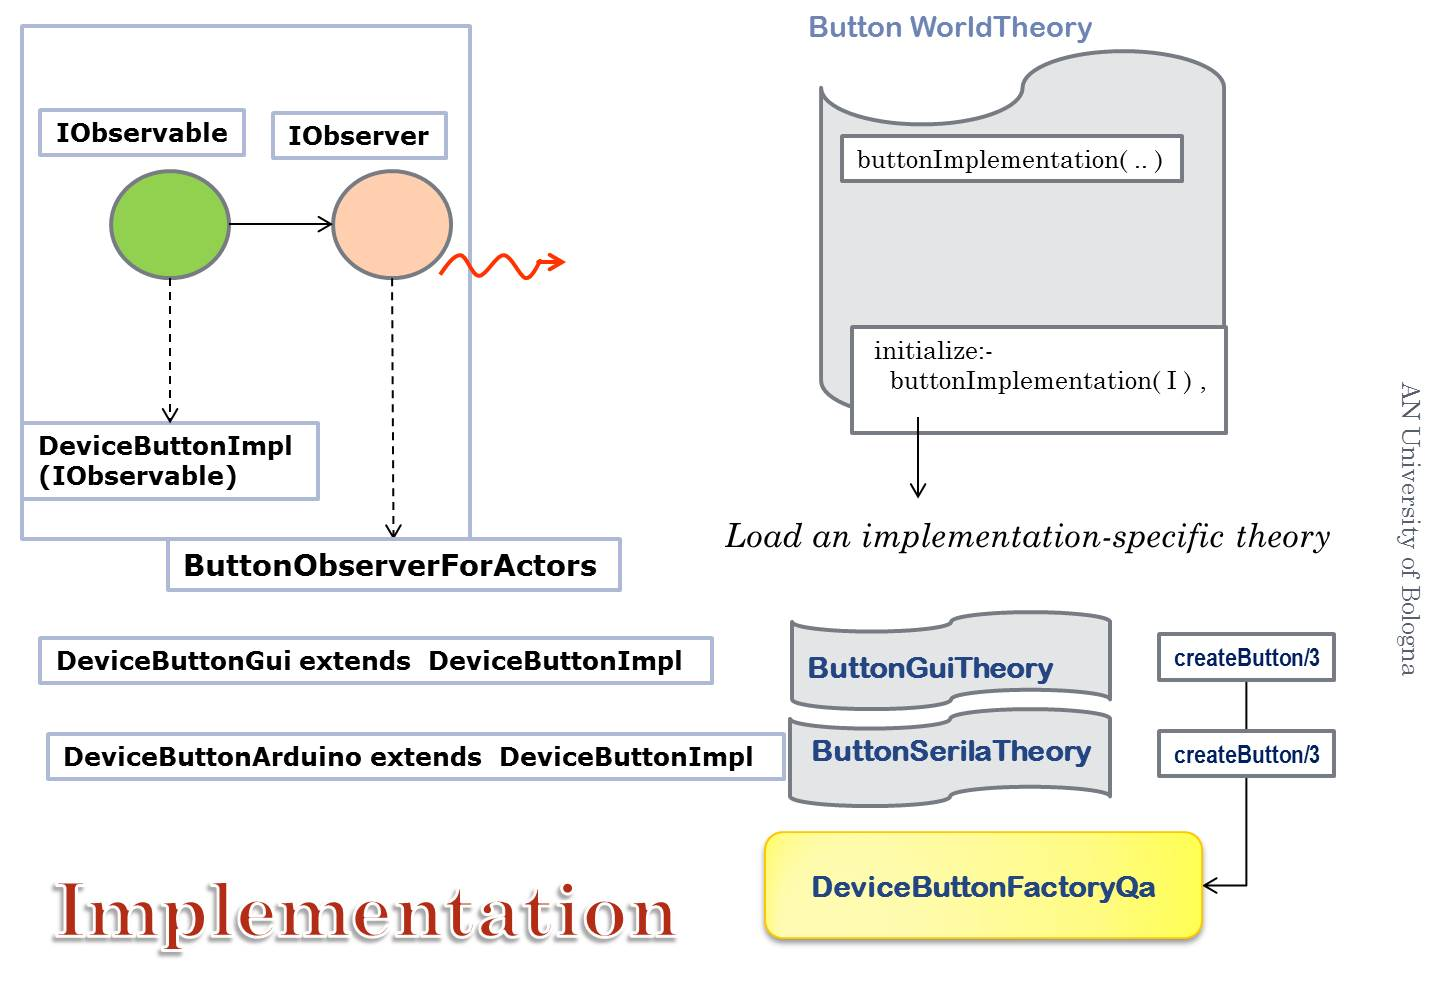
\includegraphics[scale = 0.45]{./img/buttonImplArch.jpg}\\
\end{tabular}{   }
\end{center}

The following picture shows instead the relationship between the implementation layer and the model layer:

\medskip
\begin{center}
\begin{tabular}{ c }
     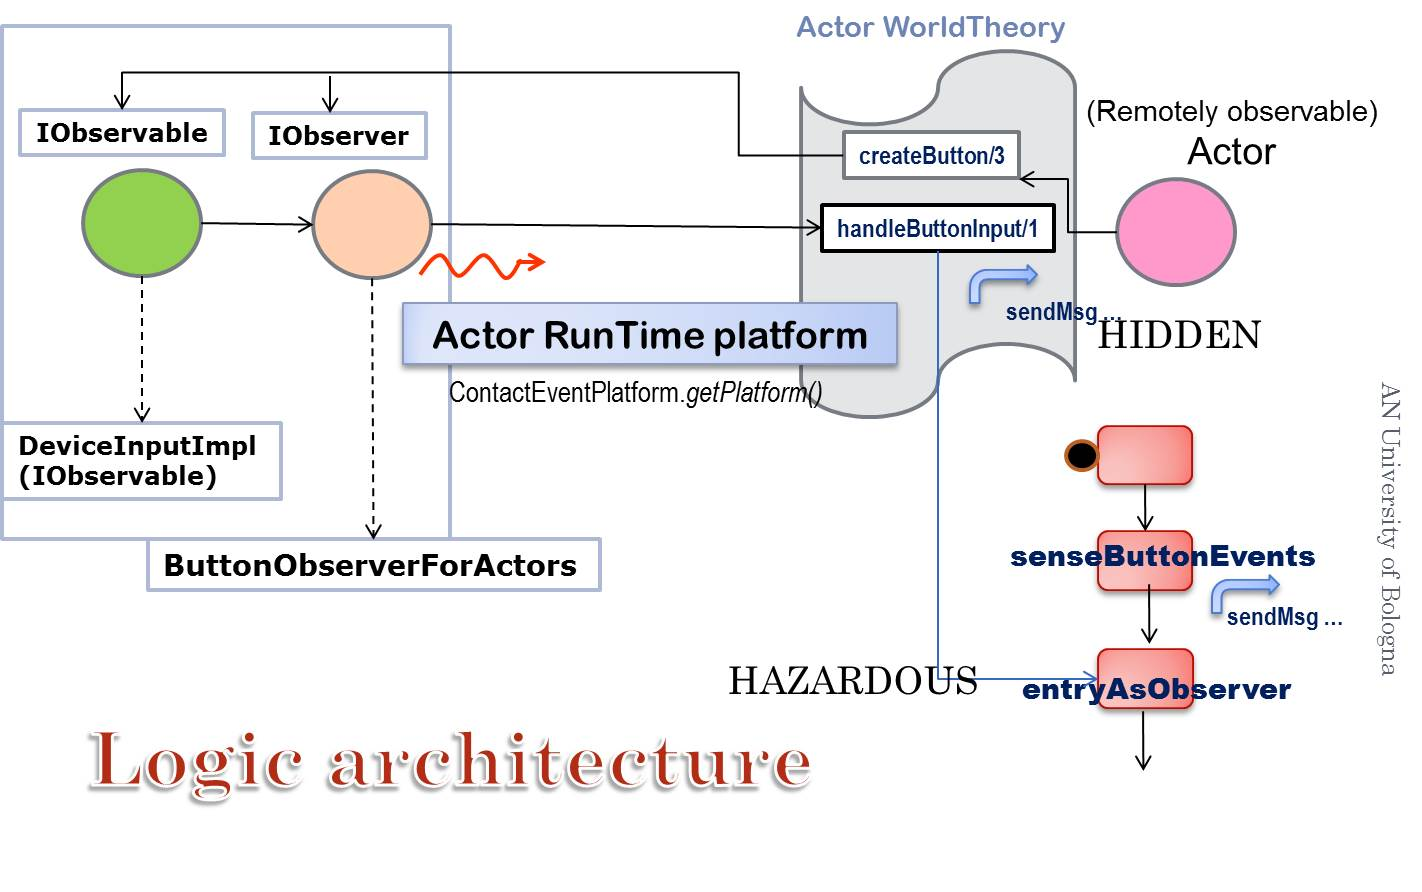
\includegraphics[scale = 0.45]{./img/buttonLogicalArchitecture.jpg}\\
\end{tabular}{   }
\end{center}

\newpage 
\section{A Button factory}
\labelssec{DeviceButtonFactoryQa}
The \java{} class \texttt{DeviceButtonFactoryQa} is a \textit{factory} that provides static methods to create a \textit{singleton} Button object and to get a reference to such an object:

\lstinputlisting[language=java,caption={ \texttt{DeviceButtonFactoryQa.java : createLedMock} }, firstline=1 , lastline=25]{../../../it.unibo.bls2016.device.qa/src/it/unibo/devices/qa/DeviceButtonFactoryQa.java}

Note that any creation method \texttt{createXXX} returns  an object of the class \texttt{DeviceButtonImpl} (see  \xss{DeviceButtonImpl} ). 

\subsection{A basic class for Button implementation}
\labelssec{DeviceButtonImpl}
The \texttt{DeviceButtonImpl} class is based on the custom framework \href{https://137.204.107.21/syskb/it.unibo.iss2015intro/docs/Frameworks/FramwCustomAppl.html}{|>>site/uniboEnv}) introduced for the rapid development of \texttt{GUI}-based prototypes.

\lstinputlisting[language=java,caption={ \texttt{DeviceButtonImpl.java} }, firstline=1 ]{../../../it.unibo.buttonLedSystemHL/src/it/unibo/buttonLed/components/DeviceButtonImpl.java}

\subsection{A Virtual Button (implementation phase)}
A Button as a virtual device can now be introduced as follows:

%%\lstinputlisting[language=java,caption={ \texttt{DeviceButtonGui.java} }, firstline=1 ]{../../../it.unibo.buttonLedSystem.gui/src/it/unibo/buttonLedSystem/gui/DeviceButtonGui.java}

The result is shown in the following picture:

\begin{center}
\begin{tabular}{ c }
     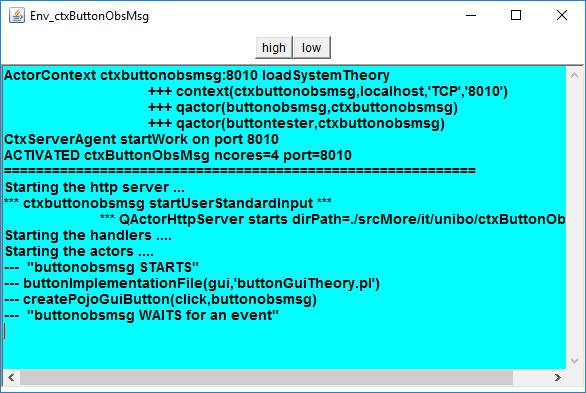
\includegraphics[scale = 0.45]{./img/buttonGui.jpg}\\
\end{tabular}{   }
\end{center}

In order to 'inject' this new implementation of the Button into our logical component, we define the theory \texttt{buttonGuiTheory} with a specific \texttt{createButton/3} rule: 


\lstinputlisting[language=ddr,caption={ \texttt{buttonGuiTheory.pl} }, firstline=1 ]{../../../it.unibo.bls2016.button/buttonGuiTheory.pl}

The next step is to introduce two new rules in  the \texttt{buttonTheory} of \xss{buttonTheory}:

%%\begin{Verbatim}[fontsize=\scriptsize, frame=single , label=Facts related to \texttt{ButtonGui} in \texttt{buttonTheory	}]
\begin{lstlisting}
buttonImplementation( gui ).
...
buttonImplementationFile( gui,  "buttonGuiTheory.pl"   ).
\end{lstlisting}
%%\end{Verbatim}

Finally, we introduce a new button creation operation in the entry in the \texttt{DeviceButtonFactoryQa}:
\lstinputlisting[language=java,caption={ \texttt{DeviceButtonFactoryQa.java : createButtonGui} }, firstline=27 , lastline=36]{../../../it.unibo.bls2016.device.qa/src/it/unibo/devices/qa/DeviceButtonFactoryQa.java}


\newpage 
\section{A Button on Arduino (implementation phase)}

An input device such as the Button can be managed in Arduino in two ways: by polling or via interrupt. 

\subsection{Managing a Button by polling.\\} 

\lstinputlisting[language=java,caption={ \texttt{buttonPolling.ino}}, firstline=1  ]{../../../it.unibo.arduino.intro/Arduino/programs/buttonPolling/buttonPolling.ino} 

\subsection{Managing a Button via interrupt.\\} 

\lstinputlisting[language=java,caption={ \texttt{buttonInterrupt.ino}}, firstline=1  ]{../../../it.unibo.arduino.intro/Arduino/programs/buttonInterrupt/buttonInterrupt.ino} 

\subsection{Managing a Button for qa message-interaction\\} 

\lstinputlisting[language=java,caption={ \texttt{button3Msg.ino}}, firstline=1  ]{../../../it.unibo.arduino.intro/Arduino/programs/button3Msg/button3Msg.ino} 

\subsection{DeviceButtonArduinoProxy}
The class \texttt{DeviceButtonArduinoProxy} creates an object that converts the observed messages coming from an \texttt{Arduino} port  into \texttt{qa} \textit{events} according to the arguments given at creation time:

\lstinputlisting[language=java,caption={ \texttt{DeviceButtonArduinoProxy.java} }, firstline=1 ]{../../../it.unibo.bls2016.device.qa/src/it/unibo/devices/qa/DeviceButtonArduinoProxy.java}

\subsection{Using the serial line in the actor}
In order to 'inject' this new implementation of the Button into our logical component, we define the theory \texttt{buttonSerialTheory} with a specific \texttt{createButton/3} rule: 


\lstinputlisting[language=ddr,caption={ \texttt{buttonGuiTheory.pl} }, firstline=1 ]{../../../it.unibo.bls2016.button/buttonSerialTheory.pl}

The next step is to introduce two new rules in  the \texttt{buttonTheory} of \xss{buttonTheory}:

%%\begin{Verbatim}[fontsize=\scriptsize, frame=single , label=Facts related to \texttt{ButtonGui} in \texttt{buttonTheory	}]
\begin{lstlisting}
buttonImplementation( arduino ).
...
buttonImplementationFile( arduino,  "buttonSerialTheory.pl"   ).
\end{lstlisting}
%%\end{Verbatim}

Finally, we introduce a new button creation operation in the entry in the \texttt{DeviceButtonFactoryQa}:
\lstinputlisting[language=java,caption={ \texttt{DeviceButtonFactoryQa.java : createButtonSerialProxy} }, firstline=47 , lastline=54]{../../../it.unibo.bls2016.device.qa/src/it/unibo/devices/qa/DeviceButtonFactoryQa.java}


 

\newpage 
\section{A Button on Raspberry (implementation phase)}
In this example, one terminal of the Button is connected to the \texttt{5V} pin (physical pin 2) while the other one (button-input pin) to pin \texttt{24} in \texttt{BCM} code. A resistor  of \texttt{10K} ohm\footnote{10K colors: brown, black, orange and argent/gold} )  is also inserted between the input pin and a \texttt{GND} pin (e.g. physical pin 9) to assure a connection to the ground when the button is not pressed.

\subsection{Button control using files}
The basic way provided by Linux to manage a device connected on a \texttt{GPIO} pin is reading/writing some (virtual) file associated with that pin.

\lstinputlisting[language=ddr,caption={ \texttt{buttonOn24Click.sh} }, firstline=1 ]{../../../it.unibo.raspIntro/src/it/unibo/bls/bash/buttonOn24Click.sh}



\subsection{Button control using the \texttt{GPIO} shell library}
The \texttt{gpio} library allows us to write a program (bash file) that reads the button-input pin and writes a \texttt{0/1} value on the Led pin:

\lstinputlisting[language=ddr,caption={ \texttt{button24Gpio.sh} }, firstline=1 ]{../../../it.unibo.raspIntro/src/it/unibo/bls/bash/gpio/button24Gpio.sh}

\subsection{Button control using python}
The Python library that handles interfacing with the \texttt{GPIO} pins allows us to write:

\lstinputlisting[language=ddr,caption={ \texttt{buttonPython24.py} }, firstline=1 ]{../../../it.unibo.raspIntro/src/it/unibo/bls/python/buttonPython24.py}



\subsection{Button control using Pi4j}
The \texttt{Pi4J} library (see \href{https://137.204.107.21/syskb/it.unibo.iss2015intro/docs/Raspberry/pi4j.html}{|>>site/Pi4j}) can be used as our \textit{technology assumption} for the implementation a \java{} class for the control of a Button connected to some pin of a Raspberry Pi:

\lstinputlisting[language=java,caption={ \texttt{DeviceLedPi4j.java} }, firstline=1 , lastline=55]{../../../it.unibo.buttonLedSystem.raspberry/src/it/unibo/bls/raspberry/components/DeviceButtonPi4j.java}

\subsection{Using the Button Pi4j in the actor}
In order to 'inject' this new implementation of the Led into our logical component, we define the theory \texttt{buttonPi4jTheory.pl}:

\lstinputlisting[language=ddr,caption={ \texttt{ledPi4jTheory.pl} }, firstline=1 ]{../../../it.unibo.bls2016.button/buttonPi4jTheory.pl}

The next step is to introduce two new rules in  the \texttt{ledTheory} of \xss{ledTheory}:

%%\begin{Verbatim}[fontsize=\scriptsize, frame=single , label=Facts related to \texttt{LedMock} in \texttt{ledTheory	}]
\begin{lstlisting}
buttonImplementation( rasp ).
...
buttonImplementationFile( rasp, "buttonPi4jTheory.pl"  ).
\end{lstlisting}
%%\end{Verbatim}

 

Finally, we introduce a new button creation operation in the entry in the \texttt{DeviceButtonFactoryQa}:
\lstinputlisting[language=java,caption={ \texttt{DeviceButtonFactoryQa.java : createButtonPi4j} }, firstline=38 , lastline=45]{../../../it.unibo.bls2016.device.qa/src/it/unibo/devices/qa/DeviceButtonFactoryQa.java}

\newpage 
\section{A Button as an observable}
\labelsec{btnobservable}
 
In our first actor-based model (see \xss{buttonasactor}) the button sends a message to a single (remote) actor. In that case, our effort was focussed on the relationship between the button-actor and the embedded button-\texttt{POJO}. In particular, the button-\texttt{POJO} has been conceived as an observable (\texttt{GOF}) object, and the \texttt{ButtonObserverForActors} defined in \xss{bobsqa} has been introduced to perform (when the button changes its state) two basic actions:
\begin{enumerate}
\item emit an event \texttt{eventId:eventMsg} (values given at creation time)  ;
\item solve the goal \texttt{handleButtonInput/1} in order to delegate to the button-actor the handling of the current button state.
\end{enumerate}

Therefore, our button-actor \texttt{buttonobsmsg} is already able to interact with any other local or remote actor that decides to sense the \texttt{eventId:eventMsg}.  In other words, the button-actor is already 'observable' by other actors, thanks to the underlying \texttt{qa} event support.

In the following model we want modify the behaviour of our button so that is becomes also able to interact with \texttt{P2P} messages with other actors that explicitly manifest (via a 'registration') their intention to receive updating massages.

\lstinputlisting[language=ddr,caption={ \texttt{buttonObservable.qa} }, firstline=1, lastline=43]{../../../it.unibo.bls2016.button/src/buttonObservable.qa}

The \texttt{buttonobservable} does not need to know its observers. The observers can be dynamically added to a system(see \xs{dynsys}) that initially starts with the Button as unique component. When the Button registers an observer,  the knowledge-base about the current system configuration is shown by the operation \texttt{showSystemConfiguration} introduced in \xss{sysconfshow}.

When the (embedded \texttt{POJO}) button changes its state, the \texttt{entryAsObserver} Plan is called and the Button sends an asynchronous  message to each registered observer as specified in the   \texttt{updateOps} rule of the \texttt{observableTheory}:

\lstinputlisting[language=pl,caption={ \texttt{observableTheory.pl} }, firstline=1,lastline=25]{../../../it.unibo.bls2016.button/observableTheory.pl}

 
To test the \texttt{buttonObservable} we can introduce some local observer actor:

\lstinputlisting[language=ddr,caption={ \texttt{buttonObservable.qa: an observer} }, firstline=45, lastline=55]{../../../it.unibo.bls2016.button/src/buttonObservable.qa}


\subsection{A Led as an observer}

Now that we have extended the \texttt{GOF} observer pattern to a distributed environment, we can dynamically introduce (see \xs{dynsys}) a remote Led that works as a button observer, by looking either at  messages or at  events.

\lstinputlisting[language=ddr,caption={ \texttt{ledAsObserver.qa} }, firstline=1 ]{../../../it.unibo.bls2016.button.observer/src/ledAsObserver.qa}

\newpage 
\section{Towards dynamic systems}
\labelsec{dynsys}
The flag \texttt{-standalone} in the declaration of a Context indicates that all the actors defined in that context must be considered external to the current system and (perhaps) already in existence. Thus, the  actors defined in a \texttt{-standalone} Context are 'place holders' for reference purposes (e.g. message passing, that requires a reference to an actor name).

The ButtonLed introduced in \xs{btnobservable} is an example of a dynamic system that can be incrementally expanded. The first logical step consists in activating the Button as a (standalone) observable entity. In the next step, a number of Leds  can be activated, each working (in its own computational) node as an observer that must 'register' itself to the Button. 


\subsection{Updating the system knowledge base}
\labelssec{sysconfkb}

Each time that a new component is dynamically added to the system, the system knowledge-base stored in each Context\footnote{The static part of the system knowledge is stored in a file \texttt{projectname,pl} generated  in the Context package of the directory \texttt{srcMore}.} is dynamically extended by the \texttt{qa} run-time support with the configuration 	related to the new component.
%
In this way, each actor in the system becomes able to send messages to other remote actors (dynamically introduced in the system), if it is able to know their names\footnote{The \texttt{register} message sent by a Led to the Button is the way used to make the Button aware of the name of the Led.} 

With reference to the ButtonLed, the initial knowledge-base related to the observable Button\footnote{The initial knowledge-base of the Button is generated in the file \textit{srcMore/it/unibo/ctxButtonObservable/buttonobservable.pl}}  is: 

\lstinputlisting[language=pl,caption={ \texttt{buttonobservable.pl of ctxButtonObservable} }, firstline=1,lastline=24]{../../../it.unibo.bls2016.button/srcMore/it/unibo/ctxButtonObservable/buttonobservable.pl}


The initial knowledge-base related to a Led\footnote{The initial knowledge-base of the observer Led is generated in the file \textit{srcMore/it/unibo/ctxLedAsObserver/ledasobserver.pl}} is:

\lstinputlisting[language=pl,caption={ \texttt{ledasobserver.pl of ctxLedAsObserver } }, firstline=1]{../../../it.unibo.bls2016.button.observer/srcMore/it/unibo/ctxLedAsObserver/ledasobserver.pl}


\subsection{Getting the system-configuration at application level}
\labelssec{sysconfshow}

The knowledge about a context configuration can be acquired at application level by rules like the following ones:

\lstinputlisting[language=pl,caption={ \texttt{observableTheory.pl} }, firstline=26]{../../../it.unibo.bls2016.button/observableTheory.pl}
 
When the Led is added to the system,  the knowledge-base of the Button is shown as follows\footnote{The actors whose names stars with \texttt{evlpa} are internal actors of class \texttt{EventLoopActors} that implement event-handling including system events.} :

\begin{lstlisting}
--- CURRENT CONTEXTS:
--- context(ctxbuttonobservable,localhost,'TCP','8010')
--- context(ctxledasobserver,localhost,'TCP','8043')
--- CURRENT ACTORS:
--- qactor(buttonobservable,ctxbuttonobservable)
--- qactor(btnobserver1,ctxbuttonobservable)
--- qactor(evlpactxbuttonobservable,ctxbuttonobservable)
--- qactor(ledobserver,ctxledasobserver)
--- qactor(evlpactxledasobserver,ctxledasobserver)
\end{lstlisting}

The same knowledge-base is updated in the Led site (and all in the other nodes dynamically added to the system).

\newpage 
\section{A system based on events}
The button-\texttt{POJO} embedded in the Button actor is an observable (\texttt{GOF}) object associated with a 'listener' (\texttt{ButtonObserverForActors}, see \xss{bobsqa}) that emits an event \texttt{eventId:eventMsg} (values given at creation time).
%
Therefore, our button-actor is already an 'observable' entity and any other local or remote actor that decides to sense the \texttt{eventId:eventMsg} can be work as a button observer.   

Thus, the logical architecture of the ButtonLed system can be redefined as follows.

\subsection{The Button as an event emitter}
The Button can be defined as an actor that emits the event \texttt{clicked:clicked(click)}. A first prototype (useful in our first sprint review) can be introduces by selecting the \texttt{GUI} implementation of the Button:   

\lstinputlisting[language=ddr,caption={ The Button as an event emitter \texttt{buttonEvent.qa} }, firstline=1 ]{../../../it.unibo.bls2016.button/src/buttonEvent.qa}

The Button Plan (state) \texttt{senseButtonEvents} does not perform here any interesting action and could be completely omitted. However, a more significant Button behaviour is introduced in \xs{usemqtt}.

Since the Button can be observed by any new component that decides to perceive the \texttt{clicked} event we can immediately starts to run the button without any observer:

\begin{tabular}{|c|c|}
\hline 
The Button & The Led \\ 
\hline 
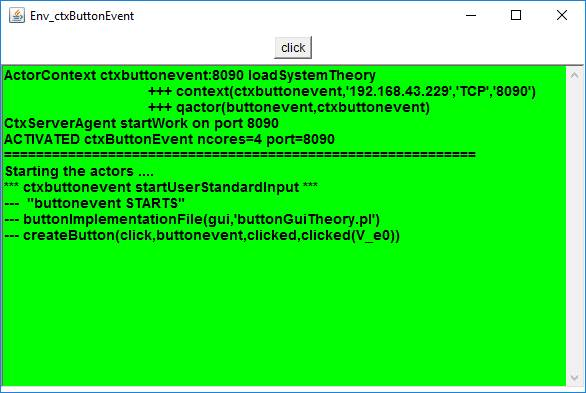
\includegraphics[scale = 0.4]{./img/buttonEventGui.jpg}
  &  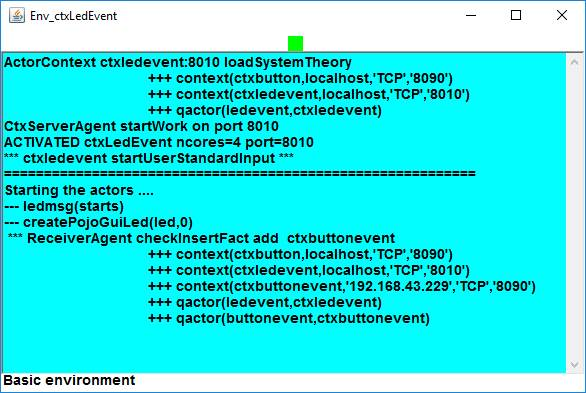
\includegraphics[scale = 0.40]{./img/ledEventGui.jpg} \\
\hline 
\end{tabular} 
\subsection{The Led as an event perceiver}
The Led can be defined as actor that waits for a clicked event and then, when the event is perceived, switches its state. Also in this case our first prototype is based on the \texttt{GUI} implementation of the Led:

\lstinputlisting[language=ddr,caption={ \texttt{ledEvent.qa} }, firstline=1 ]{../../../it.unibo.bls2016.led/src/ledEvent.qa}

Note that the button context is declared as \texttt{-standalone}. In this case we do not introduce any place holder (for the Button) since we don't have any direct interaction with it.
 
\newpage 
\section{A Button on Android}
\labelsec{buttonandroid} 
The \texttt{ButtonObserverForActors} of \xss{bobsqa} is a 'listener' that we can add also to a Button-\texttt{POJO} implemented on an Android system. According to our work-plan, we can introduce the following (in \texttt{SCRUM} terminology) \textit{product-backlog}:

\begin{itemize}
\item update the \texttt{buttonTheory} of \xss{buttonTheory} by introducing new facts related to the implementation of a Button-\texttt{POJO} in a Android environment:

%%\begin{Verbatim}[fontsize=\scriptsize, frame=single , label=Facts related to \texttt{ButtonGui} in \texttt{buttonTheory	}]
\begin{lstlisting}
buttonImplementation( android ).
...
buttonImplementationFile( gui,  "buttonAndroidTheory.pl"   ).
\end{lstlisting}
%%\end{Verbatim}

\item define the \texttt{buttonAndroidTheory}:
\lstinputlisting[language=ddr,caption={ \texttt{buttonAndroidTheory.pl} }, firstline=1 ]{../../../it.unibo.android.button.qa/assets/it/unibo/buttonqaandroid/buttonAndroidTheory.pl}

The rule \texttt{createButton/3} does not use any more the \texttt{class("...") <- op(...)} mechanism\footnote{ The \texttt{tuProlog} requires some modification of usage (see tuProlog manual, section \texttt{3.4}) in an Android environment} , but explicitly delegates the creation of the button to an operation (\texttt{createButton})  to be defined by the application designer within the actor so to adapt this task to the rules of the Android environment.

\item define an implementation for the button for Android as a specialization of the class \texttt{DeviceButtonImpl} of \xss{DeviceButtonImpl}.

\end{itemize}

\subsection{The implementation}

For the sake of simplicity, we do not use  any more the \texttt{DeviceButtonFactoryQa} of \xss{DeviceButtonFactoryQa}. Rather, we do introduce a factory method (\texttt{createButtonAndroid}) in the class \textit{DeviceButtonAndroid}. 

\lstinputlisting[language=java,caption={ \texttt{DeviceButtonAndroid.java} }, firstline=1 ]{../../../it.unibo.android.button.qa/src/it/unibo/android/button/DeviceButtonAndroid.java}

This factory method is called by the \texttt{createButton} operation that should be defined by the Application designer in the generated button implementation class \texttt{Buttonqaandroid}:

\lstinputlisting[language=java,caption={ \texttt{Buttonqaandroid.java} }, firstline=1 ]{../../../it.unibo.android.button.qa/src/it/unibo/buttonqaandroid/Buttonqaandroid.java}

The class \texttt{Buttonqaandroid} is generated only once, as a specialized version of an abstract class that implements the behaviour defined in the model.

\subsection{A model}
\labelssec{androqamodel}
Let us introduce here model similar to that of \xs{btnobservable}:

\lstinputlisting[language=ddr,caption={ \texttt{buttonAndroid.qa} }, firstline=1 ]{../../../it.unibo.android.button.qa/src/buttonAndroid.qa}

\bigskip 
\subsection{The software factory under Android}

Let us start by creating a new Android Application Project\footnote{We suppose to work in \textit{Eclipse/Xtext} extended with the \texttt{qa} plugins.}. 

\medskip   
\begin{tabular}{|c|c|}
\hline 
Android Application project 1 & Android Application project 2 \\ 
\hline 
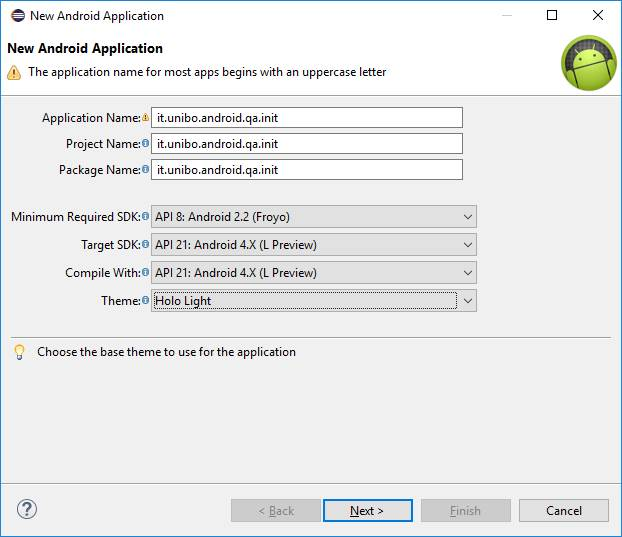
\includegraphics[scale = 0.45]{./img/qainitAndroid0.jpg}
  &  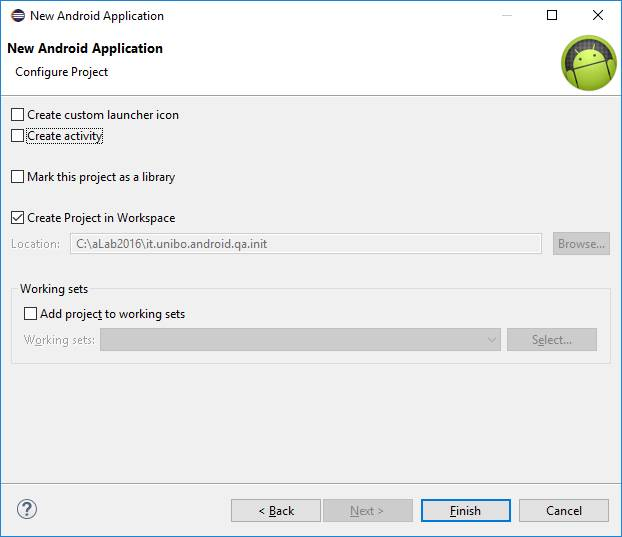
\includegraphics[scale = 0.45]{./img/qainitAndroid1.jpg} \\
\hline 
\end{tabular} 
\medskip 

If we introduce a \texttt{qa} model, a set of resources is generated, including a file \textit{AndroidManifestCustom.xml} whose content must replace the content of the \textit{AndroidManifest.xml} generated by the \texttt{AIDE} (Android \texttt{IDE}):

\medskip 
\begin{tabular}{|c|c|}
\hline 
Define a \texttt{qa} model & Code generated \\ 
\hline 
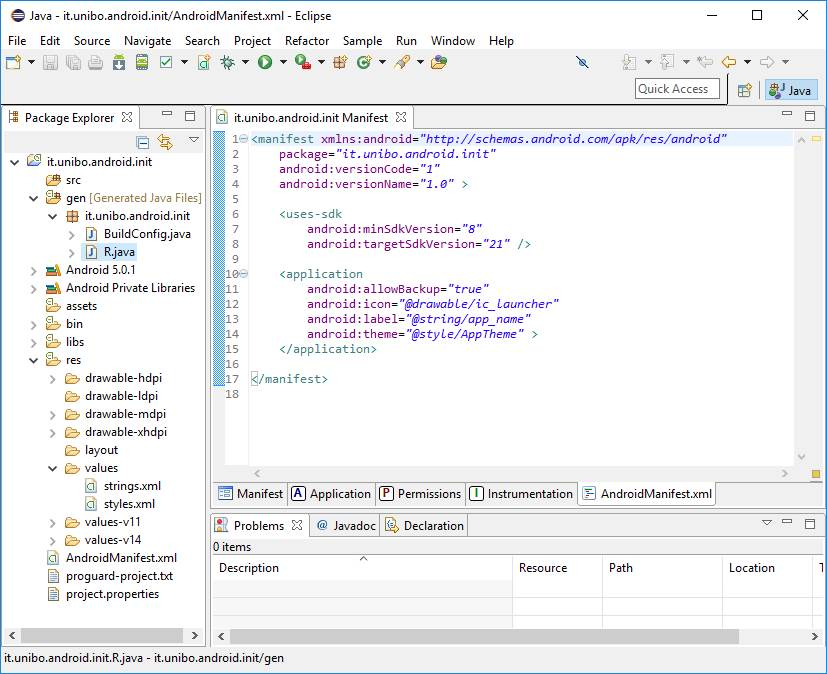
\includegraphics[scale = 0.35]{./img/qainitAndroid2.jpg}
  &  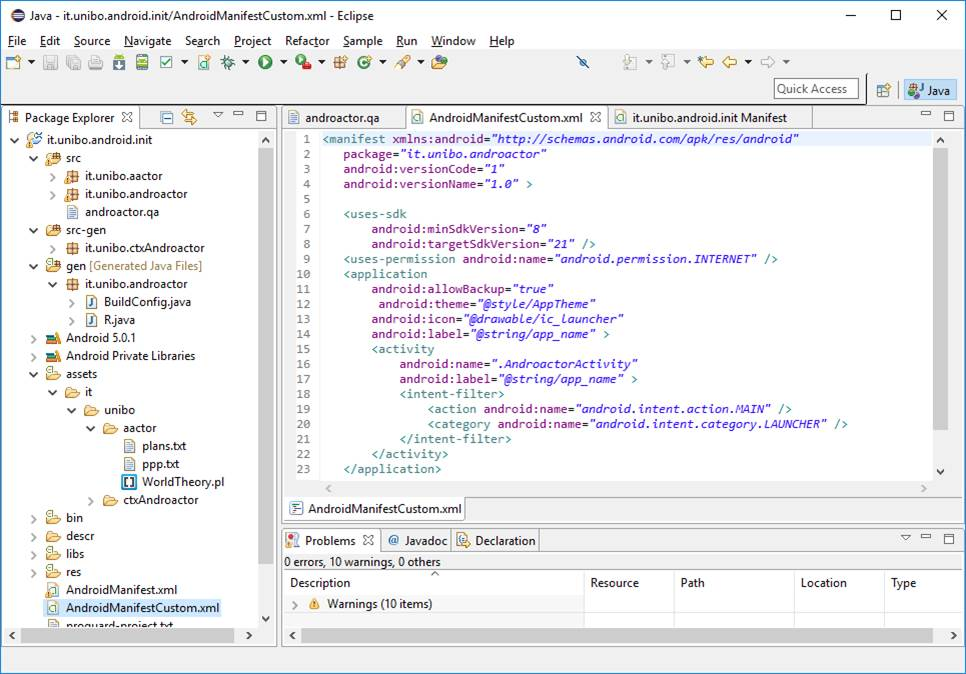
\includegraphics[scale = 0.30]{./img/qainitAndroid3.jpg} \\
\hline 
\end{tabular}
\medskip 

Note that the \texttt{srcMore} directory now does not exist any more; its content is now generated in the \texttt{assets} Android directory.
Moreover, a \texttt{xml} file (whose name \textbf{\textit{must}} be written in lower-case letters) is now generated in the Android directory \texttt{res/layout} to include the specification of a 'standard' \texttt{GUI} for the \texttt{qa} application, that forces an updating (by the  \texttt{AIDE})of the \texttt{R.java} file in the \texttt{gen} directory.
  
In the  \texttt{src} directory we can find an Activity (that extends the generated \texttt{BaseActivity} class), that defines the skeleton of the main application activity. This activity is generated only once; the task of the Application designer is to complete this code according to application needs.

Here is the structure of the project workspace for the model of \xss{androqamodel}.

\textbf{Project workspace.}\\
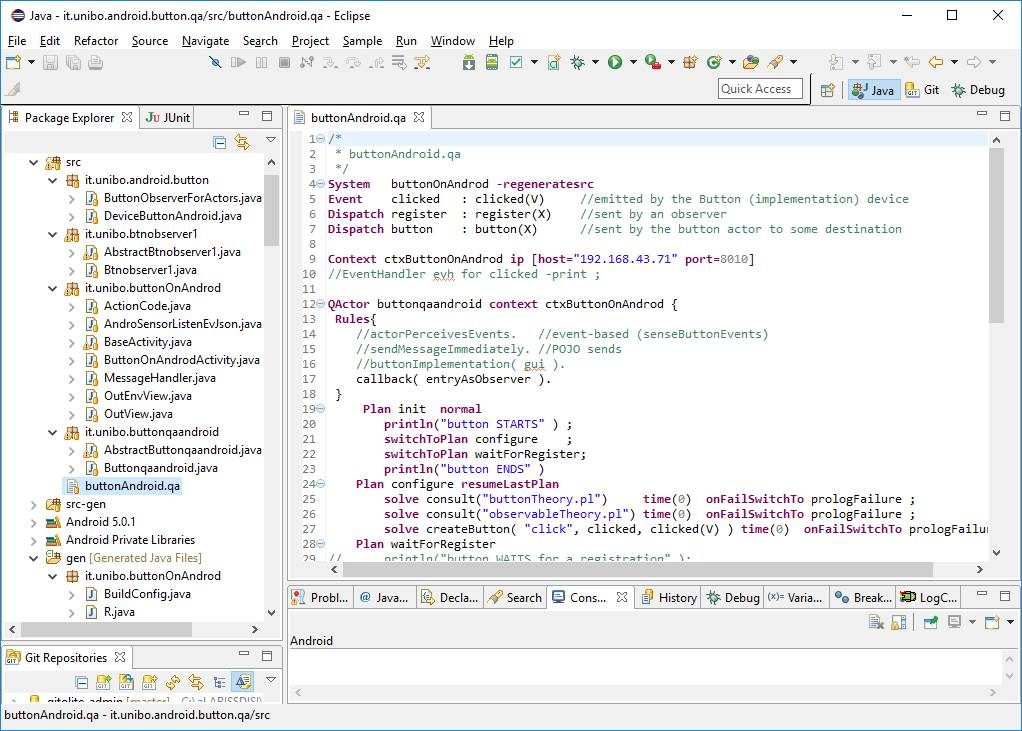
\includegraphics[scale = 0.40]{./img/qainitAndroid4.jpg}
 

\textbf{Libraries involved.} \\
 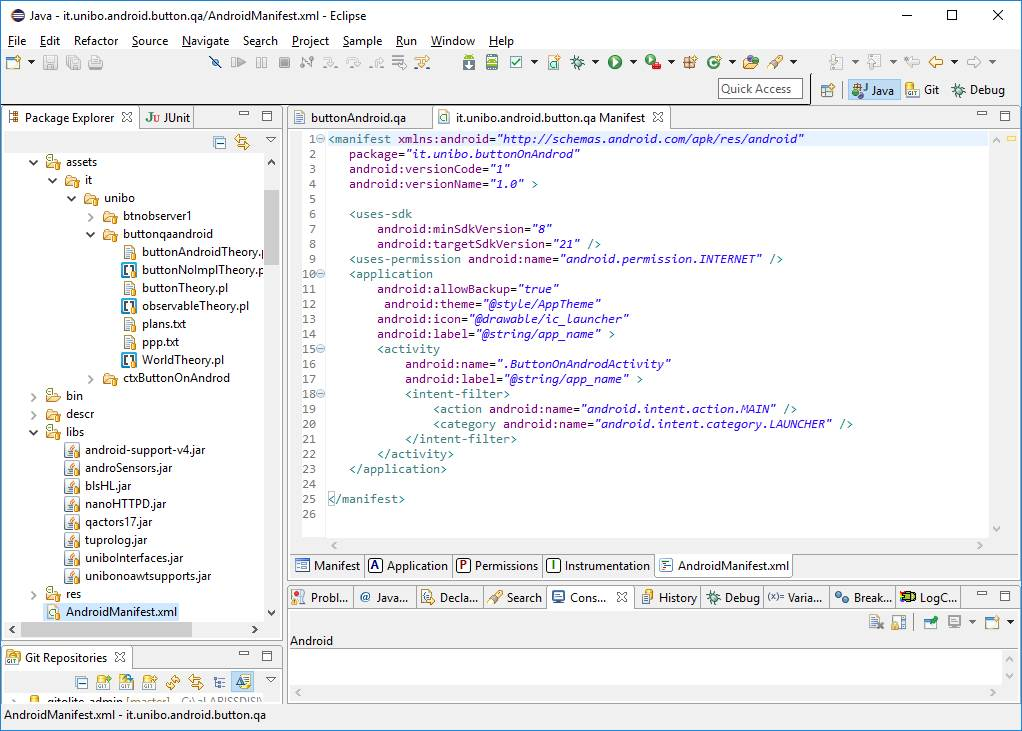
\includegraphics[scale = 0.40]{./img/qainitAndroid5.jpg}
 

\newpage 
\section{Interactions using \texttt{MQTT}}
\labelsec{usemqtt}
In this section we will redesign the remotely-observable Button of \xs{btnobservable} as an actor that works also as a \textit{publisher} of information  by using the \texttt{MQTT} protocol.

The \texttt{MQ} \textit{Telemetry Transport} (\texttt{MQTT}) is an ISO standard (ISO/IEC PRF 20922) publish-subscribe based "light weight" messaging protocol for use on top of the TCP/IP protocol. It is useful for connections with remote locations where a small code footprint is required and/or network bandwidth is at a premium.

The \textit{Eclipse Paho} project provides open-source client implementations of \texttt{MQTT} and \texttt{MQTT-SN} (\textit{MQTT For Sensor Networks}\footnote{\texttt{MQTT-SN} is a protocol derived from \texttt{MQTT}, designed for connectionless underlying network transports such as \texttt{UDP}}) messaging protocols aimed at new, existing, and emerging applications for \textit{Machine-to-Machine} (\texttt{M2M}) and \textit{Internet of Things} (\texttt{IoT}). There are already \texttt{MQTT} \texttt{C} and \java{} libraries with \texttt{Lua}, \texttt{Python}, \texttt{C++} and \texttt{JavaScript} at various stages of development.

\subsection{The Button as a \texttt{MQTT} publisher}
The remotely-observable Button introduced in \xs{btnobservable} is here extended (see the Plan \texttt{configure} and the Plan \texttt{entryAsObserver}) to become (when it changes its state) a \texttt{MQTT} publisher of information on the topic \texttt{"unibo/button/qa"}.

\lstinputlisting[language=ddr,caption={ The Button as a \texttt{MQTT} publisher \texttt{buttonMqtt.qa} }, firstline=1 ]{../../../it.unibo.bls2016.button.mqtt/src/buttonMqtt.qa}

The usage of the \texttt{MQTT} protocol is delegated to rules defined by the application designer in the \texttt{mqttTheory}. These rules in their turn make use of a \java{} utility object of class \texttt{MqttUtils}.

\subsection{The MqttUtils}
The \java{} utility class to be used as a support for \texttt{MQTT} interaction can be defined as follows:

\lstinputlisting[language=java,caption={ The utility class \texttt{MqttUtils.java} }, firstline=1 ]{../../../it.unibo.bls2016.button.mqtt/src/it/unibo/mqtt/utils/MqttUtils.java}

An object of class \texttt{MqttUtils} is used as a \textit{singleton} and works as the support for the actor that calls the operation \texttt{connect} (that creates a \texttt{MqttClient}).

The \texttt{subscribe} operation sets this singleton support as the object that provides the callback (\texttt{messageArrived}) to be called when the \texttt{MqttClient} is a subscriber. The callback is defined so to map a \texttt{MqttMessage} into a dispatch of the form:

\begin{Verbatim}[fontsize=\scriptsize, frame=single]
mqttmsg : mqttmsg( TOPIC,PAYLOAD )
\end{Verbatim}

This dispatch is then sent to the actor that uses the singleton support, i.e. that works as a \texttt{MqttClient} (subscriber).

\subsection{The mqttTheory}
The \texttt{mqttTheory} that 'extends' the \texttt{qa} action-set with new operations for the usage of the \texttt{MQTT} protocol can be defined as follows:

\lstinputlisting[language=pl,caption={ The \texttt{mqttTheory.pl} }, firstline=1 ]{../../../it.unibo.bls2016.button.mqtt/mqttTheory.pl}



\subsection{A Button observer as a \texttt{MQTT} subscriber}
To test the behaviour of our new Button-publisher, let us introduce an observer as a \texttt{MQTT} subscriber:

\lstinputlisting[language=ddr,caption={ \texttt{observerMqtt.qa} }, firstline=1 ]{../../../it.unibo.bls2016.button.mqtt/src/observerMqtt.qa}

\subsection{A Button observable actor} 
\labelssec{btnmodelandroid}
Of course we can introduce also a conventional actor that works as a Button observer via the 'registration' mechanism of \xs{btnobservable}:

\lstinputlisting[language=ddr,caption={ \texttt{observerQa.qa} }, firstline=1 ]{../../../it.unibo.bls2016.button.observer/src/observerQa.qa}




\newpage 
\section{From the components to the systems}
\labelsec{tosystem}




 
\section{Overcoming static configurations}
In the \qa{} metamodel, a software system is made of a collections of \textit{Actors}, each included in a computational node called \textit{Context}. A \textit{Context} can be viewed as a \textit{subsystem} with a unique name and a unique IP address (host,port).

In several applications, the set of \textit{Contexts} and actors that compose the system can be statically fixed, but there are other cases in which a system must dynamically change its configuration. In particular:

\begin{enumerate}
\item we should allow an actor to dynamically create other actors (actor instances) within its \textit{Context};
\item we should allow the dynamic introduction of new \textit{Contexts} within a given system, together with the possibility to support the interaction among all the actors, both statically defined and dynamically created.
\end{enumerate}


\section{Dynamic creation of actors within a Context}
Let us introduce the model of a very simple actor that receives and prints 2 messages and sends a reply to the sender;
 
\lstinputlisting[language=java,caption={ \texttt{agentprototype.qa} }, firstline=1  ]{../../../it.unibo.qactor.dynamic/src/agentprototype.qa}

This actor has the 'static' name \texttt{agentprototype}, but it refers to its own name with the built-in rule \texttt{actorobj/1}. The generated code provides (in the directory \texttt{src}) the class \texttt{Agentprototype} that defines the following constructor:

\begin{Verbatim}[fontsize=\scriptsize, frame=single , label=Constrcutor in class \textit{it.unibo.agentprototype.Agentprototype}]
public Agentprototype(String actorId, ActorContext myCtx, IOutputEnvView outEnvView )  throws Exception{
...
} 
\end{Verbatim}

This constructor can be used to build new instances in a dynamical way, by using an actor-creation rule already defined in the built-in actor's \texttt{WorldTheory}:

\subsection{An actor-creation rule}
\lstinputlisting[language=ddr,caption={ \texttt{createActor rule (in \texttt{WorldTheory})} }, firstline=33,lastline=41]{../../../it.unibo.qactor.dynamic/pivotTheory.pl}

The rule calls the constructor of the prototype given in the argument \texttt{PrototypeClass} by using the same context and the same output view of the creator's agent. Thus each new instance is always creted in the context of the creator agent.

\subsection{An actor-instance creator}
For example, the following actor \texttt{agentcreator} dynamically generates two instances of \texttt{agentprototype} and sends to each instance a messages, waiting for a reply:

\lstinputlisting[language=ddr,caption={ \texttt{agentcreation.qa} }, firstline=1]{../../../it.unibo.qactor.dynamic/src/agentcreation.qa}


The guard 
\texttt{[!? newName(agentprototype,Name,N)]} 
in Plan \texttt{createInstance} makes reference to the built-in \texttt{newname} rule for instance-names creation, that stores in the actor's knowledge base a fact \texttt{instance/3}:

\lstinputlisting[language=ddr,caption={ instance fact }, firstline=63,lastline=63]{../../../it.unibo.qactor.dynamic/pivotTheory.pl}


\subsection{The name-creation rule}
The \texttt{newname/3} name creation rule is defined in the \textit{WorldTheory} as follows:

\lstinputlisting[language=ddr,caption={ \texttt{newName rule (in \texttt{WorldTheory})} }, firstline=47,lastline=60]{../../../it.unibo.qactor.dynamic/pivotTheory.pl}

\section{Dynamic addition of Contexts}

In this section we give an example of a dynamic system that starts from a single actor (and thus from a single node) called \texttt{pivot}. Other actors can interact with \texttt{pivot} by asking it to perform two basic operations:

\begin{itemize}
\item \textit{\textbf{register(NickName,Name)}}: the actor of name \texttt{Name} informs \texttt{pivot} of its existence by providing a \textit{NickName} that can be used by other actors to find the actor;
\item \textit{\textbf{getactor(NickName)}}: the actor makes a query to \texttt{pivot} in order to obtain the (name of the) actor that corresponds to the given \texttt{NickName}. The answer given by \texttt{pivot} can be used as destination in message-passing operations.
\end{itemize}

With these two basic operations, we can extends a systems with new actors working in different nodes and we can allow an actor to interact with another one, just knowing its nickname. 

\subsection{A first dynamic actor}
In the following example:

\begin{enumerate}
\item an actor (\texttt{agent1}) registers itself to the \texttt{pivot} with the nickname \texttt{zorro};
\item \texttt{agent1} makes a request to  \texttt{pivot} for an actor with nickname \texttt{batman};
\item  \texttt{agent1} forwards a \textit{dispatch} to the actor given in the answer to its request.
\end{enumerate}

\lstinputlisting[language=ddr,caption={ \texttt{agent1.qa} }, firstline=1 , lastline=46]{../../../it.unibo.qactor.dynamic/src/agent1.qa}

Of course, this kind of system can work only if all the dynamic agents share a common knowledge about the messages that can exchange among them.

 
\subsection{A second dynamic actor}
Each dynamic agent starts from a system composed of two actors (and contexts): itself and \texttt{pivot}. 

Thus, the structural part of the model of the '\texttt{batman}' agent is quite similar to that of  \texttt{agent1} above; as regards the behaviour, we suppose here that '\texttt{batman}' first registers itself to the \texttt{pivot} and then waits for messages:

\lstinputlisting[language=ddr,caption={ \texttt{agent2.qa} }, firstline=1 , lastline=46]{../../../it.unibo.qactor.dynamic/src/agent2.qa}

Of course, \texttt{agent2} must run before \texttt{agent1} since \texttt{agent1} must find it already registered in the system.
 
\section{The pivot }
Le us introduce now a possible model for the \texttt{pivot} :
 

\lstinputlisting[language=ddr,caption={ \texttt{pivot.qa} }, firstline=1 , lastline=44]{../../../it.unibo.qactor.dynamic.pivot/src/pivot.qa}

\subsection{The pivot application theory}
Several operations of the \texttt{pivot} actor are implemented as \tuprolog{} rules by means of the user-defined \textit{pivotTheory}:

\lstinputlisting[language=java,caption={ \texttt{pivotTheory.pl} }, firstline=1 ,lastline=27 ]{../../../it.unibo.qactor.dynamic/pivotTheory.pl}
 
\subsection{The pivot at start-up} 

\begin{Verbatim}[fontsize=\scriptsize, frame=single , label=Startup]
sudo crontab -u root -e

@reboot cd /home/pi/nat/pivot && screen sh -c './pivot.sh ; read'

#!/bin/bash
echo hello pivot
sudo java -jar  MainCtxPivot.jar 
exec bash
\end{Verbatim}	



%%\begin{Verbatim}[fontsize=\scriptsize, frame=single , label=Arduino code site]
%%  
%%\end{Verbatim}

 
%%% \lstinputlisting[language=java,caption={ \texttt{DeviceButtonArduinoQa.java} }, firstline=1 , lastline=24]{../../src/it/unibo/devices/qa/DeviceButtonArduinoQa.java}

\medskip 
\scriptsize
\framebox[15cm]{ %
\begin{minipage}{140mm}
\end{minipage}}
\normalsize
\medskip 

%% \bibliographystyle{abbrv}
%% \bibliography{../biblio}

\end{document}